\documentclass{beamer}
\usepackage{tikz}

\usetheme{Singapore}
\usecolortheme{lily}
\beamertemplatenavigationsymbolsempty

\author{\textbf{Paulius Dilkas}\inst{1} \and Vaishak Belle\inst{1,2}}
\title{Generating Random Logic Programs Using Constraint Programming}
\date{CP 2020}
\institute{\inst{1} University of Edinburgh, Edinburgh, UK \and \inst{2} Alan
  Turing Institute, London, UK}

\begin{document}

\begin{frame}[noframenumbering,plain]
  \tikz[remember picture,overlay]{
    \node at ([yshift=25pt,xshift=30pt]current page.south)
    {
\includegraphics[height=40pt]{inf.png}};
    \node at ([yshift=25pt,xshift=75pt]current page.south)
    {
\includegraphics[height=40pt]{ecr.jpg}};
    \node at ([yshift=20pt,xshift=140pt]current page.south)
    {
\includegraphics[height=20pt]{epsrc.png}};
  }
  \titlepage
\end{frame}

% TODO: examples of programs

% TODO: clauses as trees

\begin{frame}{}
  \centering
  % Created by tikzDevice version 0.12.3 on 2020-01-25 19:17:02
% !TEX encoding = UTF-8 Unicode
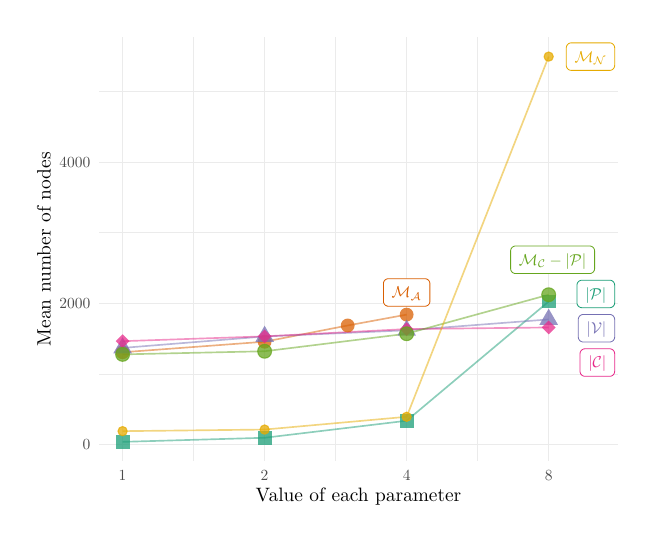
\begin{tikzpicture}[x=1pt,y=1pt]
\definecolor{fillColor}{RGB}{255,255,255}
\path[use as bounding box,fill=fillColor,fill opacity=0.00] (0,0) rectangle (216.81,176.16);
\begin{scope}
\path[clip] ( 25.78, 19.53) rectangle (213.31,172.66);
\definecolor{drawColor}{gray}{0.92}

\path[draw=drawColor,line width= 0.2pt,line join=round] ( 25.78, 51.08) --
	(213.31, 51.08);

\path[draw=drawColor,line width= 0.2pt,line join=round] ( 25.78,102.07) --
	(213.31,102.07);

\path[draw=drawColor,line width= 0.2pt,line join=round] ( 25.78,153.07) --
	(213.31,153.07);

\path[draw=drawColor,line width= 0.2pt,line join=round] ( 59.96, 19.53) --
	( 59.96,172.66);

\path[draw=drawColor,line width= 0.2pt,line join=round] (111.28, 19.53) --
	(111.28,172.66);

\path[draw=drawColor,line width= 0.2pt,line join=round] (162.60, 19.53) --
	(162.60,172.66);

\path[draw=drawColor,line width= 0.4pt,line join=round] ( 25.78, 25.58) --
	(213.31, 25.58);

\path[draw=drawColor,line width= 0.4pt,line join=round] ( 25.78, 76.58) --
	(213.31, 76.58);

\path[draw=drawColor,line width= 0.4pt,line join=round] ( 25.78,127.57) --
	(213.31,127.57);

\path[draw=drawColor,line width= 0.4pt,line join=round] ( 34.30, 19.53) --
	( 34.30,172.66);

\path[draw=drawColor,line width= 0.4pt,line join=round] ( 85.62, 19.53) --
	( 85.62,172.66);

\path[draw=drawColor,line width= 0.4pt,line join=round] (136.94, 19.53) --
	(136.94,172.66);

\path[draw=drawColor,line width= 0.4pt,line join=round] (188.26, 19.53) --
	(188.26,172.66);
\definecolor{drawColor}{RGB}{27,158,119}

\path[draw=drawColor,draw opacity=0.50,line width= 0.6pt,line join=round] ( 34.30, 26.49) --
	( 85.62, 27.97) --
	(136.94, 34.12) --
	(188.26, 77.20);
\definecolor{drawColor}{RGB}{217,95,2}

\path[draw=drawColor,draw opacity=0.50,line width= 0.6pt,line join=round] ( 34.30, 58.87) --
	( 85.62, 62.68) --
	(115.64, 68.55) --
	(136.94, 72.47);
\definecolor{drawColor}{RGB}{117,112,179}

\path[draw=drawColor,draw opacity=0.50,line width= 0.6pt,line join=round] ( 34.30, 60.44) --
	( 85.62, 64.58) --
	(136.94, 66.81) --
	(188.26, 70.73);
\definecolor{drawColor}{RGB}{231,41,138}

\path[draw=drawColor,draw opacity=0.50,line width= 0.6pt,line join=round] ( 34.30, 62.87) --
	( 85.62, 64.62) --
	(136.94, 67.25) --
	(188.26, 67.83);
\definecolor{drawColor}{RGB}{102,166,30}

\path[draw=drawColor,draw opacity=0.50,line width= 0.6pt,line join=round] ( 34.30, 58.10) --
	( 85.62, 59.23) --
	(136.94, 65.57) --
	(188.26, 79.66);
\definecolor{drawColor}{RGB}{230,171,2}

\path[draw=drawColor,draw opacity=0.50,line width= 0.6pt,line join=round] ( 34.30, 30.36) --
	( 85.62, 30.94) --
	(136.94, 35.55) --
	(188.26,165.70);
\definecolor{fillColor}{RGB}{27,158,119}

\path[fill=fillColor,fill opacity=0.75] ( 31.81, 23.99) --
	( 36.80, 23.99) --
	( 36.80, 28.99) --
	( 31.81, 28.99) --
	cycle;

\path[fill=fillColor,fill opacity=0.75] ( 83.13, 25.47) --
	( 88.12, 25.47) --
	( 88.12, 30.46) --
	( 83.13, 30.46) --
	cycle;

\path[fill=fillColor,fill opacity=0.75] (134.45, 31.63) --
	(139.44, 31.63) --
	(139.44, 36.62) --
	(134.45, 36.62) --
	cycle;

\path[fill=fillColor,fill opacity=0.75] (185.77, 74.70) --
	(190.76, 74.70) --
	(190.76, 79.69) --
	(185.77, 79.69) --
	cycle;
\definecolor{fillColor}{RGB}{217,95,2}

\path[fill=fillColor,fill opacity=0.75] ( 34.30, 58.87) circle (  2.50);

\path[fill=fillColor,fill opacity=0.75] ( 85.62, 62.68) circle (  2.50);

\path[fill=fillColor,fill opacity=0.75] (115.64, 68.55) circle (  2.50);

\path[fill=fillColor,fill opacity=0.75] (136.94, 72.47) circle (  2.50);
\definecolor{fillColor}{RGB}{117,112,179}

\path[fill=fillColor,fill opacity=0.75] ( 34.30, 64.32) --
	( 37.67, 58.50) --
	( 30.94, 58.50) --
	cycle;

\path[fill=fillColor,fill opacity=0.75] ( 85.62, 68.46) --
	( 88.99, 62.64) --
	( 82.26, 62.64) --
	cycle;

\path[fill=fillColor,fill opacity=0.75] (136.94, 70.70) --
	(140.31, 64.87) --
	(133.58, 64.87) --
	cycle;

\path[fill=fillColor,fill opacity=0.75] (188.26, 74.62) --
	(191.63, 68.79) --
	(184.90, 68.79) --
	cycle;
\definecolor{fillColor}{RGB}{231,41,138}

\path[fill=fillColor,fill opacity=0.75] ( 31.81, 62.87) --
	( 34.30, 65.37) --
	( 36.80, 62.87) --
	( 34.30, 60.37) --
	cycle;

\path[fill=fillColor,fill opacity=0.75] ( 83.13, 64.62) --
	( 85.62, 67.11) --
	( 88.12, 64.62) --
	( 85.62, 62.12) --
	cycle;

\path[fill=fillColor,fill opacity=0.75] (134.45, 67.25) --
	(136.94, 69.74) --
	(139.44, 67.25) --
	(136.94, 64.75) --
	cycle;

\path[fill=fillColor,fill opacity=0.75] (185.77, 67.83) --
	(188.26, 70.32) --
	(190.76, 67.83) --
	(188.26, 65.33) --
	cycle;
\definecolor{drawColor}{RGB}{102,166,30}
\definecolor{fillColor}{RGB}{102,166,30}

\path[draw=drawColor,draw opacity=0.75,line width= 0.4pt,line join=round,line cap=round,fill=fillColor,fill opacity=0.75] ( 34.30, 58.10) circle (  2.50);

\path[draw=drawColor,draw opacity=0.75,line width= 0.4pt,line join=round,line cap=round,fill=fillColor,fill opacity=0.75] ( 85.62, 59.23) circle (  2.50);

\path[draw=drawColor,draw opacity=0.75,line width= 0.4pt,line join=round,line cap=round,fill=fillColor,fill opacity=0.75] (136.94, 65.57) circle (  2.50);

\path[draw=drawColor,draw opacity=0.75,line width= 0.4pt,line join=round,line cap=round,fill=fillColor,fill opacity=0.75] (188.26, 79.66) circle (  2.50);
\definecolor{drawColor}{RGB}{230,171,2}
\definecolor{fillColor}{RGB}{230,171,2}

\path[draw=drawColor,draw opacity=0.75,line width= 0.4pt,line join=round,line cap=round,fill=fillColor,fill opacity=0.75] ( 34.30, 30.36) circle (  1.67);

\path[draw=drawColor,draw opacity=0.75,line width= 0.4pt,line join=round,line cap=round,fill=fillColor,fill opacity=0.75] ( 85.62, 30.94) circle (  1.67);

\path[draw=drawColor,draw opacity=0.75,line width= 0.4pt,line join=round,line cap=round,fill=fillColor,fill opacity=0.75] (136.94, 35.55) circle (  1.67);

\path[draw=drawColor,draw opacity=0.75,line width= 0.4pt,line join=round,line cap=round,fill=fillColor,fill opacity=0.75] (188.26,165.70) circle (  1.67);
\end{scope}
\begin{scope}
\path[clip] ( 25.78, 19.53) rectangle (213.31,172.66);

\path[] (198.49, 79.80) -- (188.26, 77.20);
\definecolor{drawColor}{RGB}{27,158,119}
\definecolor{fillColor}{RGB}{255,255,255}

\path[draw=drawColor,line width= 0.3pt,line join=round,line cap=round,fill=fillColor] (200.30, 74.97) --
	(210.30, 74.97) --
	(210.23, 74.97) --
	(210.52, 74.98) --
	(210.80, 75.04) --
	(211.07, 75.14) --
	(211.33, 75.29) --
	(211.55, 75.47) --
	(211.74, 75.69) --
	(211.90, 75.94) --
	(212.01, 76.20) --
	(212.08, 76.49) --
	(212.11, 76.78) --
	(212.11, 76.78) --
	(212.11, 83.11) --
	(212.11, 83.11) --
	(212.08, 83.40) --
	(212.01, 83.68) --
	(211.90, 83.94) --
	(211.74, 84.19) --
	(211.55, 84.41) --
	(211.33, 84.59) --
	(211.07, 84.74) --
	(210.80, 84.84) --
	(210.52, 84.90) --
	(210.30, 84.91) --
	(200.30, 84.91) --
	(200.52, 84.90) --
	(200.23, 84.91) --
	(199.94, 84.88) --
	(199.66, 84.79) --
	(199.40, 84.67) --
	(199.16, 84.50) --
	(198.95, 84.30) --
	(198.77, 84.07) --
	(198.64, 83.81) --
	(198.55, 83.54) --
	(198.50, 83.25) --
	(198.49, 83.11) --
	(198.49, 76.78) --
	(198.50, 76.92) --
	(198.50, 76.63) --
	(198.55, 76.34) --
	(198.64, 76.07) --
	(198.77, 75.81) --
	(198.95, 75.58) --
	(199.16, 75.38) --
	(199.40, 75.21) --
	(199.66, 75.09) --
	(199.94, 75.01) --
	(200.23, 74.97) --
	cycle;
\end{scope}
\begin{scope}
\path[clip] ( 25.78, 19.53) rectangle (213.31,172.66);
\definecolor{drawColor}{RGB}{27,158,119}

\node[text=drawColor,anchor=base,inner sep=0pt, outer sep=0pt, scale=  0.57] at (205.30, 77.98) {$|\mathcal{P}|$};
\end{scope}
\begin{scope}
\path[clip] ( 25.78, 19.53) rectangle (213.31,172.66);

\path[] (198.97, 67.74) -- (188.26, 70.73);
\definecolor{drawColor}{RGB}{117,112,179}
\definecolor{fillColor}{RGB}{255,255,255}

\path[draw=drawColor,line width= 0.3pt,line join=round,line cap=round,fill=fillColor] (200.77, 62.58) --
	(210.30, 62.58) --
	(210.23, 62.58) --
	(210.52, 62.59) --
	(210.80, 62.65) --
	(211.07, 62.75) --
	(211.33, 62.90) --
	(211.55, 63.08) --
	(211.74, 63.30) --
	(211.90, 63.54) --
	(212.01, 63.81) --
	(212.08, 64.09) --
	(212.11, 64.38) --
	(212.11, 64.38) --
	(212.11, 70.71) --
	(212.11, 70.71) --
	(212.08, 71.00) --
	(212.01, 71.29) --
	(211.90, 71.55) --
	(211.74, 71.80) --
	(211.55, 72.02) --
	(211.33, 72.20) --
	(211.07, 72.35) --
	(210.80, 72.45) --
	(210.52, 72.51) --
	(210.30, 72.52) --
	(200.77, 72.52) --
	(200.99, 72.51) --
	(200.70, 72.52) --
	(200.41, 72.48) --
	(200.13, 72.40) --
	(199.87, 72.28) --
	(199.63, 72.11) --
	(199.42, 71.91) --
	(199.25, 71.68) --
	(199.11, 71.42) --
	(199.02, 71.15) --
	(198.97, 70.86) --
	(198.97, 70.71) --
	(198.97, 64.38) --
	(198.97, 64.53) --
	(198.97, 64.24) --
	(199.02, 63.95) --
	(199.11, 63.68) --
	(199.25, 63.42) --
	(199.42, 63.19) --
	(199.63, 62.99) --
	(199.87, 62.82) --
	(200.13, 62.70) --
	(200.41, 62.61) --
	(200.70, 62.58) --
	cycle;
\end{scope}
\begin{scope}
\path[clip] ( 25.78, 19.53) rectangle (213.31,172.66);
\definecolor{drawColor}{RGB}{117,112,179}

\node[text=drawColor,anchor=base,inner sep=0pt, outer sep=0pt, scale=  0.57] at (205.54, 65.59) {$|\mathcal{V}|$};
\end{scope}
\begin{scope}
\path[clip] ( 25.78, 19.53) rectangle (213.31,172.66);

\path[] (199.59, 56.31) -- (188.26, 67.83);
\definecolor{drawColor}{RGB}{231,41,138}
\definecolor{fillColor}{RGB}{255,255,255}

\path[draw=drawColor,line width= 0.3pt,line join=round,line cap=round,fill=fillColor] (201.40, 50.18) --
	(210.30, 50.18) --
	(210.23, 50.18) --
	(210.52, 50.19) --
	(210.80, 50.25) --
	(211.07, 50.35) --
	(211.33, 50.50) --
	(211.55, 50.68) --
	(211.74, 50.90) --
	(211.90, 51.15) --
	(212.01, 51.41) --
	(212.08, 51.70) --
	(212.11, 51.99) --
	(212.11, 51.99) --
	(212.11, 58.31) --
	(212.11, 58.31) --
	(212.08, 58.60) --
	(212.01, 58.89) --
	(211.90, 59.15) --
	(211.74, 59.40) --
	(211.55, 59.62) --
	(211.33, 59.80) --
	(211.07, 59.95) --
	(210.80, 60.05) --
	(210.52, 60.11) --
	(210.30, 60.12) --
	(201.40, 60.12) --
	(201.62, 60.11) --
	(201.33, 60.12) --
	(201.04, 60.08) --
	(200.76, 60.00) --
	(200.50, 59.88) --
	(200.26, 59.71) --
	(200.05, 59.51) --
	(199.87, 59.28) --
	(199.74, 59.02) --
	(199.65, 58.75) --
	(199.60, 58.46) --
	(199.59, 58.31) --
	(199.59, 51.99) --
	(199.60, 52.13) --
	(199.60, 51.84) --
	(199.65, 51.55) --
	(199.74, 51.28) --
	(199.87, 51.02) --
	(200.05, 50.79) --
	(200.26, 50.59) --
	(200.50, 50.42) --
	(200.76, 50.30) --
	(201.04, 50.22) --
	(201.33, 50.18) --
	cycle;
\end{scope}
\begin{scope}
\path[clip] ( 25.78, 19.53) rectangle (213.31,172.66);
\definecolor{drawColor}{RGB}{231,41,138}

\node[text=drawColor,anchor=base,inner sep=0pt, outer sep=0pt, scale=  0.57] at (205.85, 53.19) {$|\mathcal{C}|$};
\end{scope}
\begin{scope}
\path[clip] ( 25.78, 19.53) rectangle (213.31,172.66);

\path[] (189.67, 87.32) -- (188.26, 79.66);
\definecolor{drawColor}{RGB}{102,166,30}
\definecolor{fillColor}{RGB}{255,255,255}

\path[draw=drawColor,line width= 0.3pt,line join=round,line cap=round,fill=fillColor] (176.31, 87.32) --
	(203.05, 87.32) --
	(202.98, 87.32) --
	(203.27, 87.33) --
	(203.56, 87.39) --
	(203.83, 87.49) --
	(204.08, 87.64) --
	(204.31, 87.82) --
	(204.50, 88.04) --
	(204.65, 88.28) --
	(204.77, 88.55) --
	(204.84, 88.83) --
	(204.86, 89.12) --
	(204.86, 89.12) --
	(204.86, 95.45) --
	(204.86, 95.45) --
	(204.84, 95.74) --
	(204.77, 96.03) --
	(204.65, 96.29) --
	(204.50, 96.54) --
	(204.31, 96.76) --
	(204.08, 96.94) --
	(203.83, 97.09) --
	(203.56, 97.19) --
	(203.27, 97.25) --
	(203.05, 97.26) --
	(176.31, 97.26) --
	(176.53, 97.25) --
	(176.24, 97.26) --
	(175.95, 97.22) --
	(175.67, 97.14) --
	(175.41, 97.02) --
	(175.17, 96.85) --
	(174.96, 96.65) --
	(174.79, 96.42) --
	(174.65, 96.16) --
	(174.56, 95.89) --
	(174.51, 95.60) --
	(174.51, 95.45) --
	(174.51, 89.12) --
	(174.51, 89.27) --
	(174.51, 88.98) --
	(174.56, 88.69) --
	(174.65, 88.42) --
	(174.79, 88.16) --
	(174.96, 87.93) --
	(175.17, 87.72) --
	(175.41, 87.56) --
	(175.67, 87.44) --
	(175.95, 87.35) --
	(176.24, 87.32) --
	cycle;
\end{scope}
\begin{scope}
\path[clip] ( 25.78, 19.53) rectangle (213.31,172.66);
\definecolor{drawColor}{RGB}{102,166,30}

\node[text=drawColor,anchor=base,inner sep=0pt, outer sep=0pt, scale=  0.57] at (189.68, 90.33) {$\mathcal{M}_{\mathcal{C}}-|\mathcal{P}|$};
\end{scope}
\begin{scope}
\path[clip] ( 25.78, 19.53) rectangle (213.31,172.66);

\path[] (194.64,165.70) -- (188.26,165.70);
\definecolor{drawColor}{RGB}{230,171,2}
\definecolor{fillColor}{RGB}{255,255,255}

\path[draw=drawColor,line width= 0.3pt,line join=round,line cap=round,fill=fillColor] (196.44,160.73) --
	(210.30,160.73) --
	(210.23,160.73) --
	(210.52,160.74) --
	(210.80,160.80) --
	(211.07,160.90) --
	(211.33,161.05) --
	(211.55,161.23) --
	(211.74,161.45) --
	(211.90,161.69) --
	(212.01,161.96) --
	(212.08,162.24) --
	(212.11,162.53) --
	(212.11,162.53) --
	(212.11,168.86) --
	(212.11,168.86) --
	(212.08,169.15) --
	(212.01,169.43) --
	(211.90,169.70) --
	(211.74,169.95) --
	(211.55,170.16) --
	(211.33,170.35) --
	(211.07,170.49) --
	(210.80,170.60) --
	(210.52,170.66) --
	(210.30,170.67) --
	(196.44,170.67) --
	(196.66,170.66) --
	(196.37,170.67) --
	(196.08,170.63) --
	(195.80,170.55) --
	(195.54,170.43) --
	(195.30,170.26) --
	(195.09,170.06) --
	(194.92,169.83) --
	(194.78,169.57) --
	(194.69,169.29) --
	(194.64,169.01) --
	(194.64,168.86) --
	(194.64,162.53) --
	(194.64,162.68) --
	(194.64,162.39) --
	(194.69,162.10) --
	(194.78,161.82) --
	(194.92,161.57) --
	(195.09,161.34) --
	(195.30,161.13) --
	(195.54,160.97) --
	(195.80,160.84) --
	(196.08,160.76) --
	(196.37,160.73) --
	cycle;
\end{scope}
\begin{scope}
\path[clip] ( 25.78, 19.53) rectangle (213.31,172.66);
\definecolor{drawColor}{RGB}{230,171,2}

\node[text=drawColor,anchor=base,inner sep=0pt, outer sep=0pt, scale=  0.57] at (203.37,163.74) {$\mathcal{M}_{\mathcal{N}}$};
\end{scope}
\begin{scope}
\path[clip] ( 25.78, 19.53) rectangle (213.31,172.66);
\definecolor{drawColor}{RGB}{217,95,2}
\definecolor{fillColor}{RGB}{255,255,255}

\path[draw=drawColor,line width= 0.3pt,line join=round,line cap=round,fill=fillColor] (130.35, 75.50) --
	(143.54, 75.50) --
	(143.46, 75.51) --
	(143.75, 75.52) --
	(144.04, 75.58) --
	(144.31, 75.68) --
	(144.56, 75.82) --
	(144.79, 76.01) --
	(144.98, 76.23) --
	(145.14, 76.47) --
	(145.25, 76.74) --
	(145.32, 77.02) --
	(145.34, 77.31) --
	(145.34, 77.31) --
	(145.34, 83.64) --
	(145.34, 83.64) --
	(145.32, 83.93) --
	(145.25, 84.21) --
	(145.14, 84.48) --
	(144.98, 84.72) --
	(144.79, 84.94) --
	(144.56, 85.13) --
	(144.31, 85.27) --
	(144.04, 85.37) --
	(143.75, 85.43) --
	(143.54, 85.45) --
	(130.35, 85.45) --
	(130.57, 85.43) --
	(130.28, 85.44) --
	(129.99, 85.41) --
	(129.71, 85.33) --
	(129.45, 85.20) --
	(129.21, 85.04) --
	(129.00, 84.84) --
	(128.83, 84.61) --
	(128.69, 84.35) --
	(128.60, 84.07) --
	(128.55, 83.78) --
	(128.55, 83.64) --
	(128.55, 77.31) --
	(128.55, 77.46) --
	(128.55, 77.17) --
	(128.60, 76.88) --
	(128.69, 76.60) --
	(128.83, 76.35) --
	(129.00, 76.11) --
	(129.21, 75.91) --
	(129.45, 75.75) --
	(129.71, 75.62) --
	(129.99, 75.54) --
	(130.28, 75.51) --
	cycle;
\end{scope}
\begin{scope}
\path[clip] ( 25.78, 19.53) rectangle (213.31,172.66);
\definecolor{drawColor}{RGB}{217,95,2}

\node[text=drawColor,anchor=base,inner sep=0pt, outer sep=0pt, scale=  0.57] at (136.94, 78.52) {$\mathcal{M}_{\mathcal{A}}$};
\end{scope}
\begin{scope}
\path[clip] (  0.00,  0.00) rectangle (216.81,176.16);
\definecolor{drawColor}{gray}{0.30}

\node[text=drawColor,anchor=base east,inner sep=0pt, outer sep=0pt, scale=  0.56] at ( 22.63, 23.65) {0};

\node[text=drawColor,anchor=base east,inner sep=0pt, outer sep=0pt, scale=  0.56] at ( 22.63, 74.65) {2000};

\node[text=drawColor,anchor=base east,inner sep=0pt, outer sep=0pt, scale=  0.56] at ( 22.63,125.64) {4000};
\end{scope}
\begin{scope}
\path[clip] (  0.00,  0.00) rectangle (216.81,176.16);
\definecolor{drawColor}{gray}{0.30}

\node[text=drawColor,anchor=base,inner sep=0pt, outer sep=0pt, scale=  0.56] at ( 34.30, 12.52) {1};

\node[text=drawColor,anchor=base,inner sep=0pt, outer sep=0pt, scale=  0.56] at ( 85.62, 12.52) {2};

\node[text=drawColor,anchor=base,inner sep=0pt, outer sep=0pt, scale=  0.56] at (136.94, 12.52) {4};

\node[text=drawColor,anchor=base,inner sep=0pt, outer sep=0pt, scale=  0.56] at (188.26, 12.52) {8};
\end{scope}
\begin{scope}
\path[clip] (  0.00,  0.00) rectangle (216.81,176.16);
\definecolor{drawColor}{RGB}{0,0,0}

\node[text=drawColor,anchor=base,inner sep=0pt, outer sep=0pt, scale=  0.70] at (119.54,  4.86) {Value of each parameter};
\end{scope}
\begin{scope}
\path[clip] (  0.00,  0.00) rectangle (216.81,176.16);
\definecolor{drawColor}{RGB}{0,0,0}

\node[text=drawColor,rotate= 90.00,anchor=base,inner sep=0pt, outer sep=0pt, scale=  0.70] at (  8.32, 96.09) {Mean number of nodes};
\end{scope}
\end{tikzpicture}

\end{frame}

\begin{frame}{}
  \centering
  % Created by tikzDevice version 0.12.3 on 2020-05-11 12:49:46
% !TEX encoding = UTF-8 Unicode
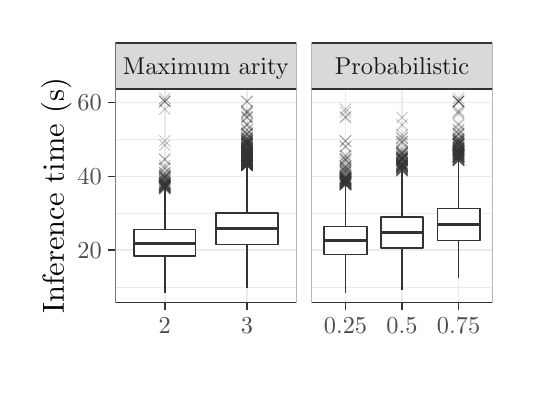
\begin{tikzpicture}[x=1pt,y=1pt]
\definecolor{fillColor}{RGB}{255,255,255}
\path[use as bounding box,fill=fillColor,fill opacity=0.00] (0,0) rectangle (173.45,130.09);
\begin{scope}
\path[clip] (  0.00,  0.00) rectangle (173.45,130.09);
\definecolor{drawColor}{RGB}{255,255,255}
\definecolor{fillColor}{RGB}{255,255,255}

\path[draw=drawColor,line width= 0.6pt,line join=round,line cap=round,fill=fillColor] ( -0.00,  0.00) rectangle (173.45,130.09);
\end{scope}
\begin{scope}
\path[clip] ( 31.71, 30.69) rectangle ( 97.08,108.01);
\definecolor{fillColor}{RGB}{255,255,255}

\path[fill=fillColor] ( 31.71, 30.69) rectangle ( 97.08,108.01);
\definecolor{drawColor}{gray}{0.92}

\path[draw=drawColor,line width= 0.3pt,line join=round] ( 31.71, 36.29) --
	( 97.08, 36.29);

\path[draw=drawColor,line width= 0.3pt,line join=round] ( 31.71, 62.99) --
	( 97.08, 62.99);

\path[draw=drawColor,line width= 0.3pt,line join=round] ( 31.71, 89.69) --
	( 97.08, 89.69);

\path[draw=drawColor,line width= 0.6pt,line join=round] ( 31.71, 49.64) --
	( 97.08, 49.64);

\path[draw=drawColor,line width= 0.6pt,line join=round] ( 31.71, 76.34) --
	( 97.08, 76.34);

\path[draw=drawColor,line width= 0.6pt,line join=round] ( 31.71,103.05) --
	( 97.08,103.05);

\path[draw=drawColor,line width= 0.6pt,line join=round] ( 49.54, 30.69) --
	( 49.54,108.01);

\path[draw=drawColor,line width= 0.6pt,line join=round] ( 79.25, 30.69) --
	( 79.25,108.01);
\definecolor{drawColor}{RGB}{51,51,51}

\path[draw=drawColor,draw opacity=0.25,line width= 0.4pt,line join=round,line cap=round] ( 47.58, 71.97) -- ( 51.50, 75.90);

\path[draw=drawColor,draw opacity=0.25,line width= 0.4pt,line join=round,line cap=round] ( 47.58, 75.90) -- ( 51.50, 71.97);

\path[draw=drawColor,draw opacity=0.25,line width= 0.4pt,line join=round,line cap=round] ( 47.58, 71.07) -- ( 51.50, 74.99);

\path[draw=drawColor,draw opacity=0.25,line width= 0.4pt,line join=round,line cap=round] ( 47.58, 74.99) -- ( 51.50, 71.07);

\path[draw=drawColor,draw opacity=0.25,line width= 0.4pt,line join=round,line cap=round] ( 47.58, 80.47) -- ( 51.50, 84.39);

\path[draw=drawColor,draw opacity=0.25,line width= 0.4pt,line join=round,line cap=round] ( 47.58, 84.39) -- ( 51.50, 80.47);

\path[draw=drawColor,draw opacity=0.25,line width= 0.4pt,line join=round,line cap=round] ( 47.58, 75.71) -- ( 51.50, 79.64);

\path[draw=drawColor,draw opacity=0.25,line width= 0.4pt,line join=round,line cap=round] ( 47.58, 79.64) -- ( 51.50, 75.71);

\path[draw=drawColor,draw opacity=0.25,line width= 0.4pt,line join=round,line cap=round] ( 47.58, 73.51) -- ( 51.50, 77.44);

\path[draw=drawColor,draw opacity=0.25,line width= 0.4pt,line join=round,line cap=round] ( 47.58, 77.44) -- ( 51.50, 73.51);

\path[draw=drawColor,draw opacity=0.25,line width= 0.4pt,line join=round,line cap=round] ( 47.58, 71.96) -- ( 51.50, 75.88);

\path[draw=drawColor,draw opacity=0.25,line width= 0.4pt,line join=round,line cap=round] ( 47.58, 75.88) -- ( 51.50, 71.96);

\path[draw=drawColor,draw opacity=0.25,line width= 0.4pt,line join=round,line cap=round] ( 47.58, 74.26) -- ( 51.50, 78.19);

\path[draw=drawColor,draw opacity=0.25,line width= 0.4pt,line join=round,line cap=round] ( 47.58, 78.19) -- ( 51.50, 74.26);

\path[draw=drawColor,draw opacity=0.25,line width= 0.4pt,line join=round,line cap=round] ( 47.58, 70.50) -- ( 51.50, 74.42);

\path[draw=drawColor,draw opacity=0.25,line width= 0.4pt,line join=round,line cap=round] ( 47.58, 74.42) -- ( 51.50, 70.50);

\path[draw=drawColor,draw opacity=0.25,line width= 0.4pt,line join=round,line cap=round] ( 47.58, 74.45) -- ( 51.50, 78.37);

\path[draw=drawColor,draw opacity=0.25,line width= 0.4pt,line join=round,line cap=round] ( 47.58, 78.37) -- ( 51.50, 74.45);

\path[draw=drawColor,draw opacity=0.25,line width= 0.4pt,line join=round,line cap=round] ( 47.58, 71.60) -- ( 51.50, 75.53);

\path[draw=drawColor,draw opacity=0.25,line width= 0.4pt,line join=round,line cap=round] ( 47.58, 75.53) -- ( 51.50, 71.60);

\path[draw=drawColor,draw opacity=0.25,line width= 0.4pt,line join=round,line cap=round] ( 47.58, 74.07) -- ( 51.50, 77.99);

\path[draw=drawColor,draw opacity=0.25,line width= 0.4pt,line join=round,line cap=round] ( 47.58, 77.99) -- ( 51.50, 74.07);

\path[draw=drawColor,draw opacity=0.25,line width= 0.4pt,line join=round,line cap=round] ( 47.58, 72.86) -- ( 51.50, 76.78);

\path[draw=drawColor,draw opacity=0.25,line width= 0.4pt,line join=round,line cap=round] ( 47.58, 76.78) -- ( 51.50, 72.86);

\path[draw=drawColor,draw opacity=0.25,line width= 0.4pt,line join=round,line cap=round] ( 47.58, 71.26) -- ( 51.50, 75.18);

\path[draw=drawColor,draw opacity=0.25,line width= 0.4pt,line join=round,line cap=round] ( 47.58, 75.18) -- ( 51.50, 71.26);

\path[draw=drawColor,draw opacity=0.25,line width= 0.4pt,line join=round,line cap=round] ( 47.58, 71.60) -- ( 51.50, 75.53);

\path[draw=drawColor,draw opacity=0.25,line width= 0.4pt,line join=round,line cap=round] ( 47.58, 75.53) -- ( 51.50, 71.60);

\path[draw=drawColor,draw opacity=0.25,line width= 0.4pt,line join=round,line cap=round] ( 47.58, 71.53) -- ( 51.50, 75.46);

\path[draw=drawColor,draw opacity=0.25,line width= 0.4pt,line join=round,line cap=round] ( 47.58, 75.46) -- ( 51.50, 71.53);

\path[draw=drawColor,draw opacity=0.25,line width= 0.4pt,line join=round,line cap=round] ( 47.58, 74.17) -- ( 51.50, 78.09);

\path[draw=drawColor,draw opacity=0.25,line width= 0.4pt,line join=round,line cap=round] ( 47.58, 78.09) -- ( 51.50, 74.17);

\path[draw=drawColor,draw opacity=0.25,line width= 0.4pt,line join=round,line cap=round] ( 47.58, 72.05) -- ( 51.50, 75.98);

\path[draw=drawColor,draw opacity=0.25,line width= 0.4pt,line join=round,line cap=round] ( 47.58, 75.98) -- ( 51.50, 72.05);

\path[draw=drawColor,draw opacity=0.25,line width= 0.4pt,line join=round,line cap=round] ( 47.58, 70.59) -- ( 51.50, 74.51);

\path[draw=drawColor,draw opacity=0.25,line width= 0.4pt,line join=round,line cap=round] ( 47.58, 74.51) -- ( 51.50, 70.59);

\path[draw=drawColor,draw opacity=0.25,line width= 0.4pt,line join=round,line cap=round] ( 47.58, 71.60) -- ( 51.50, 75.53);

\path[draw=drawColor,draw opacity=0.25,line width= 0.4pt,line join=round,line cap=round] ( 47.58, 75.53) -- ( 51.50, 71.60);

\path[draw=drawColor,draw opacity=0.25,line width= 0.4pt,line join=round,line cap=round] ( 47.58, 71.73) -- ( 51.50, 75.65);

\path[draw=drawColor,draw opacity=0.25,line width= 0.4pt,line join=round,line cap=round] ( 47.58, 75.65) -- ( 51.50, 71.73);

\path[draw=drawColor,draw opacity=0.25,line width= 0.4pt,line join=round,line cap=round] ( 47.58, 71.27) -- ( 51.50, 75.19);

\path[draw=drawColor,draw opacity=0.25,line width= 0.4pt,line join=round,line cap=round] ( 47.58, 75.19) -- ( 51.50, 71.27);

\path[draw=drawColor,draw opacity=0.25,line width= 0.4pt,line join=round,line cap=round] ( 47.58, 70.86) -- ( 51.50, 74.79);

\path[draw=drawColor,draw opacity=0.25,line width= 0.4pt,line join=round,line cap=round] ( 47.58, 74.79) -- ( 51.50, 70.86);

\path[draw=drawColor,draw opacity=0.25,line width= 0.4pt,line join=round,line cap=round] ( 47.58, 72.78) -- ( 51.50, 76.70);

\path[draw=drawColor,draw opacity=0.25,line width= 0.4pt,line join=round,line cap=round] ( 47.58, 76.70) -- ( 51.50, 72.78);

\path[draw=drawColor,draw opacity=0.25,line width= 0.4pt,line join=round,line cap=round] ( 47.58, 73.08) -- ( 51.50, 77.01);

\path[draw=drawColor,draw opacity=0.25,line width= 0.4pt,line join=round,line cap=round] ( 47.58, 77.01) -- ( 51.50, 73.08);

\path[draw=drawColor,draw opacity=0.25,line width= 0.4pt,line join=round,line cap=round] ( 47.58, 70.27) -- ( 51.50, 74.19);

\path[draw=drawColor,draw opacity=0.25,line width= 0.4pt,line join=round,line cap=round] ( 47.58, 74.19) -- ( 51.50, 70.27);

\path[draw=drawColor,draw opacity=0.25,line width= 0.4pt,line join=round,line cap=round] ( 47.58, 75.09) -- ( 51.50, 79.01);

\path[draw=drawColor,draw opacity=0.25,line width= 0.4pt,line join=round,line cap=round] ( 47.58, 79.01) -- ( 51.50, 75.09);

\path[draw=drawColor,draw opacity=0.25,line width= 0.4pt,line join=round,line cap=round] ( 47.58, 74.26) -- ( 51.50, 78.18);

\path[draw=drawColor,draw opacity=0.25,line width= 0.4pt,line join=round,line cap=round] ( 47.58, 78.18) -- ( 51.50, 74.26);

\path[draw=drawColor,draw opacity=0.25,line width= 0.4pt,line join=round,line cap=round] ( 47.58, 71.92) -- ( 51.50, 75.84);

\path[draw=drawColor,draw opacity=0.25,line width= 0.4pt,line join=round,line cap=round] ( 47.58, 75.84) -- ( 51.50, 71.92);

\path[draw=drawColor,draw opacity=0.25,line width= 0.4pt,line join=round,line cap=round] ( 47.58, 70.89) -- ( 51.50, 74.82);

\path[draw=drawColor,draw opacity=0.25,line width= 0.4pt,line join=round,line cap=round] ( 47.58, 74.82) -- ( 51.50, 70.89);

\path[draw=drawColor,draw opacity=0.25,line width= 0.4pt,line join=round,line cap=round] ( 47.58, 70.81) -- ( 51.50, 74.73);

\path[draw=drawColor,draw opacity=0.25,line width= 0.4pt,line join=round,line cap=round] ( 47.58, 74.73) -- ( 51.50, 70.81);

\path[draw=drawColor,draw opacity=0.25,line width= 0.4pt,line join=round,line cap=round] ( 47.58, 71.32) -- ( 51.50, 75.24);

\path[draw=drawColor,draw opacity=0.25,line width= 0.4pt,line join=round,line cap=round] ( 47.58, 75.24) -- ( 51.50, 71.32);

\path[draw=drawColor,draw opacity=0.25,line width= 0.4pt,line join=round,line cap=round] ( 47.58, 73.51) -- ( 51.50, 77.43);

\path[draw=drawColor,draw opacity=0.25,line width= 0.4pt,line join=round,line cap=round] ( 47.58, 77.43) -- ( 51.50, 73.51);

\path[draw=drawColor,draw opacity=0.25,line width= 0.4pt,line join=round,line cap=round] ( 47.58, 72.68) -- ( 51.50, 76.60);

\path[draw=drawColor,draw opacity=0.25,line width= 0.4pt,line join=round,line cap=round] ( 47.58, 76.60) -- ( 51.50, 72.68);

\path[draw=drawColor,draw opacity=0.25,line width= 0.4pt,line join=round,line cap=round] ( 47.58, 75.68) -- ( 51.50, 79.61);

\path[draw=drawColor,draw opacity=0.25,line width= 0.4pt,line join=round,line cap=round] ( 47.58, 79.61) -- ( 51.50, 75.68);

\path[draw=drawColor,draw opacity=0.25,line width= 0.4pt,line join=round,line cap=round] ( 47.58, 70.08) -- ( 51.50, 74.01);

\path[draw=drawColor,draw opacity=0.25,line width= 0.4pt,line join=round,line cap=round] ( 47.58, 74.01) -- ( 51.50, 70.08);

\path[draw=drawColor,draw opacity=0.25,line width= 0.4pt,line join=round,line cap=round] ( 47.58, 72.32) -- ( 51.50, 76.24);

\path[draw=drawColor,draw opacity=0.25,line width= 0.4pt,line join=round,line cap=round] ( 47.58, 76.24) -- ( 51.50, 72.32);

\path[draw=drawColor,draw opacity=0.25,line width= 0.4pt,line join=round,line cap=round] ( 47.58, 70.44) -- ( 51.50, 74.37);

\path[draw=drawColor,draw opacity=0.25,line width= 0.4pt,line join=round,line cap=round] ( 47.58, 74.37) -- ( 51.50, 70.44);

\path[draw=drawColor,draw opacity=0.25,line width= 0.4pt,line join=round,line cap=round] ( 47.58, 70.61) -- ( 51.50, 74.54);

\path[draw=drawColor,draw opacity=0.25,line width= 0.4pt,line join=round,line cap=round] ( 47.58, 74.54) -- ( 51.50, 70.61);

\path[draw=drawColor,draw opacity=0.25,line width= 0.4pt,line join=round,line cap=round] ( 47.58, 69.97) -- ( 51.50, 73.89);

\path[draw=drawColor,draw opacity=0.25,line width= 0.4pt,line join=round,line cap=round] ( 47.58, 73.89) -- ( 51.50, 69.97);

\path[draw=drawColor,draw opacity=0.25,line width= 0.4pt,line join=round,line cap=round] ( 47.58, 78.26) -- ( 51.50, 82.18);

\path[draw=drawColor,draw opacity=0.25,line width= 0.4pt,line join=round,line cap=round] ( 47.58, 82.18) -- ( 51.50, 78.26);

\path[draw=drawColor,draw opacity=0.25,line width= 0.4pt,line join=round,line cap=round] ( 47.58, 74.73) -- ( 51.50, 78.66);

\path[draw=drawColor,draw opacity=0.25,line width= 0.4pt,line join=round,line cap=round] ( 47.58, 78.66) -- ( 51.50, 74.73);

\path[draw=drawColor,draw opacity=0.25,line width= 0.4pt,line join=round,line cap=round] ( 47.58, 71.06) -- ( 51.50, 74.99);

\path[draw=drawColor,draw opacity=0.25,line width= 0.4pt,line join=round,line cap=round] ( 47.58, 74.99) -- ( 51.50, 71.06);

\path[draw=drawColor,draw opacity=0.25,line width= 0.4pt,line join=round,line cap=round] ( 47.58,101.49) -- ( 51.50,105.41);

\path[draw=drawColor,draw opacity=0.25,line width= 0.4pt,line join=round,line cap=round] ( 47.58,105.41) -- ( 51.50,101.49);

\path[draw=drawColor,draw opacity=0.25,line width= 0.4pt,line join=round,line cap=round] ( 47.58,102.54) -- ( 51.50,106.46);

\path[draw=drawColor,draw opacity=0.25,line width= 0.4pt,line join=round,line cap=round] ( 47.58,106.46) -- ( 51.50,102.54);

\path[draw=drawColor,draw opacity=0.25,line width= 0.4pt,line join=round,line cap=round] ( 47.58, 77.11) -- ( 51.50, 81.03);

\path[draw=drawColor,draw opacity=0.25,line width= 0.4pt,line join=round,line cap=round] ( 47.58, 81.03) -- ( 51.50, 77.11);

\path[draw=drawColor,draw opacity=0.25,line width= 0.4pt,line join=round,line cap=round] ( 47.58,101.45) -- ( 51.50,105.38);

\path[draw=drawColor,draw opacity=0.25,line width= 0.4pt,line join=round,line cap=round] ( 47.58,105.38) -- ( 51.50,101.45);

\path[draw=drawColor,draw opacity=0.25,line width= 0.4pt,line join=round,line cap=round] ( 47.58,101.49) -- ( 51.50,105.41);

\path[draw=drawColor,draw opacity=0.25,line width= 0.4pt,line join=round,line cap=round] ( 47.58,105.41) -- ( 51.50,101.49);

\path[draw=drawColor,draw opacity=0.25,line width= 0.4pt,line join=round,line cap=round] ( 47.58, 98.71) -- ( 51.50,102.64);

\path[draw=drawColor,draw opacity=0.25,line width= 0.4pt,line join=round,line cap=round] ( 47.58,102.64) -- ( 51.50, 98.71);

\path[draw=drawColor,draw opacity=0.25,line width= 0.4pt,line join=round,line cap=round] ( 47.58, 85.70) -- ( 51.50, 89.62);

\path[draw=drawColor,draw opacity=0.25,line width= 0.4pt,line join=round,line cap=round] ( 47.58, 89.62) -- ( 51.50, 85.70);

\path[draw=drawColor,draw opacity=0.25,line width= 0.4pt,line join=round,line cap=round] ( 47.58, 70.59) -- ( 51.50, 74.52);

\path[draw=drawColor,draw opacity=0.25,line width= 0.4pt,line join=round,line cap=round] ( 47.58, 74.52) -- ( 51.50, 70.59);

\path[draw=drawColor,draw opacity=0.25,line width= 0.4pt,line join=round,line cap=round] ( 47.58, 69.91) -- ( 51.50, 73.84);

\path[draw=drawColor,draw opacity=0.25,line width= 0.4pt,line join=round,line cap=round] ( 47.58, 73.84) -- ( 51.50, 69.91);

\path[draw=drawColor,draw opacity=0.25,line width= 0.4pt,line join=round,line cap=round] ( 47.58, 70.65) -- ( 51.50, 74.58);

\path[draw=drawColor,draw opacity=0.25,line width= 0.4pt,line join=round,line cap=round] ( 47.58, 74.58) -- ( 51.50, 70.65);

\path[draw=drawColor,draw opacity=0.25,line width= 0.4pt,line join=round,line cap=round] ( 47.58, 70.71) -- ( 51.50, 74.63);

\path[draw=drawColor,draw opacity=0.25,line width= 0.4pt,line join=round,line cap=round] ( 47.58, 74.63) -- ( 51.50, 70.71);

\path[draw=drawColor,draw opacity=0.25,line width= 0.4pt,line join=round,line cap=round] ( 47.58, 70.41) -- ( 51.50, 74.33);

\path[draw=drawColor,draw opacity=0.25,line width= 0.4pt,line join=round,line cap=round] ( 47.58, 74.33) -- ( 51.50, 70.41);

\path[draw=drawColor,draw opacity=0.25,line width= 0.4pt,line join=round,line cap=round] ( 47.58, 77.48) -- ( 51.50, 81.41);

\path[draw=drawColor,draw opacity=0.25,line width= 0.4pt,line join=round,line cap=round] ( 47.58, 81.41) -- ( 51.50, 77.48);

\path[draw=drawColor,draw opacity=0.25,line width= 0.4pt,line join=round,line cap=round] ( 47.58, 80.61) -- ( 51.50, 84.53);

\path[draw=drawColor,draw opacity=0.25,line width= 0.4pt,line join=round,line cap=round] ( 47.58, 84.53) -- ( 51.50, 80.61);

\path[draw=drawColor,draw opacity=0.25,line width= 0.4pt,line join=round,line cap=round] ( 47.58, 87.23) -- ( 51.50, 91.16);

\path[draw=drawColor,draw opacity=0.25,line width= 0.4pt,line join=round,line cap=round] ( 47.58, 91.16) -- ( 51.50, 87.23);

\path[draw=drawColor,draw opacity=0.25,line width= 0.4pt,line join=round,line cap=round] ( 47.58, 73.91) -- ( 51.50, 77.83);

\path[draw=drawColor,draw opacity=0.25,line width= 0.4pt,line join=round,line cap=round] ( 47.58, 77.83) -- ( 51.50, 73.91);
\definecolor{drawColor}{gray}{0.20}

\path[draw=drawColor,line width= 0.6pt,line join=round] ( 49.54, 57.22) -- ( 49.54, 71.81);

\path[draw=drawColor,line width= 0.6pt,line join=round] ( 49.54, 47.48) -- ( 49.54, 34.20);

\path[draw=drawColor,line width= 0.6pt,line join=round,line cap=round,fill=fillColor] ( 38.40, 57.22) --
	( 38.40, 47.48) --
	( 60.68, 47.48) --
	( 60.68, 57.22) --
	( 38.40, 57.22) --
	cycle;

\path[draw=drawColor,line width= 1.1pt,line join=round] ( 38.40, 52.13) -- ( 60.68, 52.13);
\definecolor{drawColor}{RGB}{51,51,51}

\path[draw=drawColor,draw opacity=0.25,line width= 0.4pt,line join=round,line cap=round] ( 77.29, 81.78) -- ( 81.21, 85.71);

\path[draw=drawColor,draw opacity=0.25,line width= 0.4pt,line join=round,line cap=round] ( 77.29, 85.71) -- ( 81.21, 81.78);

\path[draw=drawColor,draw opacity=0.25,line width= 0.4pt,line join=round,line cap=round] ( 77.29, 82.35) -- ( 81.21, 86.27);

\path[draw=drawColor,draw opacity=0.25,line width= 0.4pt,line join=round,line cap=round] ( 77.29, 86.27) -- ( 81.21, 82.35);

\path[draw=drawColor,draw opacity=0.25,line width= 0.4pt,line join=round,line cap=round] ( 77.29, 79.08) -- ( 81.21, 83.00);

\path[draw=drawColor,draw opacity=0.25,line width= 0.4pt,line join=round,line cap=round] ( 77.29, 83.00) -- ( 81.21, 79.08);

\path[draw=drawColor,draw opacity=0.25,line width= 0.4pt,line join=round,line cap=round] ( 77.29, 79.03) -- ( 81.21, 82.96);

\path[draw=drawColor,draw opacity=0.25,line width= 0.4pt,line join=round,line cap=round] ( 77.29, 82.96) -- ( 81.21, 79.03);

\path[draw=drawColor,draw opacity=0.25,line width= 0.4pt,line join=round,line cap=round] ( 77.29, 82.81) -- ( 81.21, 86.73);

\path[draw=drawColor,draw opacity=0.25,line width= 0.4pt,line join=round,line cap=round] ( 77.29, 86.73) -- ( 81.21, 82.81);

\path[draw=drawColor,draw opacity=0.25,line width= 0.4pt,line join=round,line cap=round] ( 77.29, 80.76) -- ( 81.21, 84.68);

\path[draw=drawColor,draw opacity=0.25,line width= 0.4pt,line join=round,line cap=round] ( 77.29, 84.68) -- ( 81.21, 80.76);

\path[draw=drawColor,draw opacity=0.25,line width= 0.4pt,line join=round,line cap=round] ( 77.29, 80.46) -- ( 81.21, 84.39);

\path[draw=drawColor,draw opacity=0.25,line width= 0.4pt,line join=round,line cap=round] ( 77.29, 84.39) -- ( 81.21, 80.46);

\path[draw=drawColor,draw opacity=0.25,line width= 0.4pt,line join=round,line cap=round] ( 77.29, 87.59) -- ( 81.21, 91.52);

\path[draw=drawColor,draw opacity=0.25,line width= 0.4pt,line join=round,line cap=round] ( 77.29, 91.52) -- ( 81.21, 87.59);

\path[draw=drawColor,draw opacity=0.25,line width= 0.4pt,line join=round,line cap=round] ( 77.29, 80.62) -- ( 81.21, 84.55);

\path[draw=drawColor,draw opacity=0.25,line width= 0.4pt,line join=round,line cap=round] ( 77.29, 84.55) -- ( 81.21, 80.62);

\path[draw=drawColor,draw opacity=0.25,line width= 0.4pt,line join=round,line cap=round] ( 77.29, 83.17) -- ( 81.21, 87.09);

\path[draw=drawColor,draw opacity=0.25,line width= 0.4pt,line join=round,line cap=round] ( 77.29, 87.09) -- ( 81.21, 83.17);

\path[draw=drawColor,draw opacity=0.25,line width= 0.4pt,line join=round,line cap=round] ( 77.29, 79.21) -- ( 81.21, 83.13);

\path[draw=drawColor,draw opacity=0.25,line width= 0.4pt,line join=round,line cap=round] ( 77.29, 83.13) -- ( 81.21, 79.21);

\path[draw=drawColor,draw opacity=0.25,line width= 0.4pt,line join=round,line cap=round] ( 77.29, 79.27) -- ( 81.21, 83.20);

\path[draw=drawColor,draw opacity=0.25,line width= 0.4pt,line join=round,line cap=round] ( 77.29, 83.20) -- ( 81.21, 79.27);

\path[draw=drawColor,draw opacity=0.25,line width= 0.4pt,line join=round,line cap=round] ( 77.29, 79.26) -- ( 81.21, 83.19);

\path[draw=drawColor,draw opacity=0.25,line width= 0.4pt,line join=round,line cap=round] ( 77.29, 83.19) -- ( 81.21, 79.26);

\path[draw=drawColor,draw opacity=0.25,line width= 0.4pt,line join=round,line cap=round] ( 77.29, 86.88) -- ( 81.21, 90.81);

\path[draw=drawColor,draw opacity=0.25,line width= 0.4pt,line join=round,line cap=round] ( 77.29, 90.81) -- ( 81.21, 86.88);

\path[draw=drawColor,draw opacity=0.25,line width= 0.4pt,line join=round,line cap=round] ( 77.29, 78.48) -- ( 81.21, 82.41);

\path[draw=drawColor,draw opacity=0.25,line width= 0.4pt,line join=round,line cap=round] ( 77.29, 82.41) -- ( 81.21, 78.48);

\path[draw=drawColor,draw opacity=0.25,line width= 0.4pt,line join=round,line cap=round] ( 77.29, 84.54) -- ( 81.21, 88.47);

\path[draw=drawColor,draw opacity=0.25,line width= 0.4pt,line join=round,line cap=round] ( 77.29, 88.47) -- ( 81.21, 84.54);

\path[draw=drawColor,draw opacity=0.25,line width= 0.4pt,line join=round,line cap=round] ( 77.29, 87.09) -- ( 81.21, 91.01);

\path[draw=drawColor,draw opacity=0.25,line width= 0.4pt,line join=round,line cap=round] ( 77.29, 91.01) -- ( 81.21, 87.09);

\path[draw=drawColor,draw opacity=0.25,line width= 0.4pt,line join=round,line cap=round] ( 77.29, 82.58) -- ( 81.21, 86.51);

\path[draw=drawColor,draw opacity=0.25,line width= 0.4pt,line join=round,line cap=round] ( 77.29, 86.51) -- ( 81.21, 82.58);

\path[draw=drawColor,draw opacity=0.25,line width= 0.4pt,line join=round,line cap=round] ( 77.29, 86.17) -- ( 81.21, 90.09);

\path[draw=drawColor,draw opacity=0.25,line width= 0.4pt,line join=round,line cap=round] ( 77.29, 90.09) -- ( 81.21, 86.17);

\path[draw=drawColor,draw opacity=0.25,line width= 0.4pt,line join=round,line cap=round] ( 77.29, 86.00) -- ( 81.21, 89.93);

\path[draw=drawColor,draw opacity=0.25,line width= 0.4pt,line join=round,line cap=round] ( 77.29, 89.93) -- ( 81.21, 86.00);

\path[draw=drawColor,draw opacity=0.25,line width= 0.4pt,line join=round,line cap=round] ( 77.29, 81.62) -- ( 81.21, 85.54);

\path[draw=drawColor,draw opacity=0.25,line width= 0.4pt,line join=round,line cap=round] ( 77.29, 85.54) -- ( 81.21, 81.62);

\path[draw=drawColor,draw opacity=0.25,line width= 0.4pt,line join=round,line cap=round] ( 77.29, 89.72) -- ( 81.21, 93.64);

\path[draw=drawColor,draw opacity=0.25,line width= 0.4pt,line join=round,line cap=round] ( 77.29, 93.64) -- ( 81.21, 89.72);

\path[draw=drawColor,draw opacity=0.25,line width= 0.4pt,line join=round,line cap=round] ( 77.29, 84.29) -- ( 81.21, 88.21);

\path[draw=drawColor,draw opacity=0.25,line width= 0.4pt,line join=round,line cap=round] ( 77.29, 88.21) -- ( 81.21, 84.29);

\path[draw=drawColor,draw opacity=0.25,line width= 0.4pt,line join=round,line cap=round] ( 77.29, 83.16) -- ( 81.21, 87.08);

\path[draw=drawColor,draw opacity=0.25,line width= 0.4pt,line join=round,line cap=round] ( 77.29, 87.08) -- ( 81.21, 83.16);

\path[draw=drawColor,draw opacity=0.25,line width= 0.4pt,line join=round,line cap=round] ( 77.29, 80.29) -- ( 81.21, 84.22);

\path[draw=drawColor,draw opacity=0.25,line width= 0.4pt,line join=round,line cap=round] ( 77.29, 84.22) -- ( 81.21, 80.29);

\path[draw=drawColor,draw opacity=0.25,line width= 0.4pt,line join=round,line cap=round] ( 77.29, 78.56) -- ( 81.21, 82.49);

\path[draw=drawColor,draw opacity=0.25,line width= 0.4pt,line join=round,line cap=round] ( 77.29, 82.49) -- ( 81.21, 78.56);

\path[draw=drawColor,draw opacity=0.25,line width= 0.4pt,line join=round,line cap=round] ( 77.29, 90.11) -- ( 81.21, 94.04);

\path[draw=drawColor,draw opacity=0.25,line width= 0.4pt,line join=round,line cap=round] ( 77.29, 94.04) -- ( 81.21, 90.11);

\path[draw=drawColor,draw opacity=0.25,line width= 0.4pt,line join=round,line cap=round] ( 77.29, 83.43) -- ( 81.21, 87.35);

\path[draw=drawColor,draw opacity=0.25,line width= 0.4pt,line join=round,line cap=round] ( 77.29, 87.35) -- ( 81.21, 83.43);

\path[draw=drawColor,draw opacity=0.25,line width= 0.4pt,line join=round,line cap=round] ( 77.29, 82.66) -- ( 81.21, 86.58);

\path[draw=drawColor,draw opacity=0.25,line width= 0.4pt,line join=round,line cap=round] ( 77.29, 86.58) -- ( 81.21, 82.66);

\path[draw=drawColor,draw opacity=0.25,line width= 0.4pt,line join=round,line cap=round] ( 77.29, 83.00) -- ( 81.21, 86.93);

\path[draw=drawColor,draw opacity=0.25,line width= 0.4pt,line join=round,line cap=round] ( 77.29, 86.93) -- ( 81.21, 83.00);

\path[draw=drawColor,draw opacity=0.25,line width= 0.4pt,line join=round,line cap=round] ( 77.29, 79.39) -- ( 81.21, 83.31);

\path[draw=drawColor,draw opacity=0.25,line width= 0.4pt,line join=round,line cap=round] ( 77.29, 83.31) -- ( 81.21, 79.39);

\path[draw=drawColor,draw opacity=0.25,line width= 0.4pt,line join=round,line cap=round] ( 77.29, 83.28) -- ( 81.21, 87.20);

\path[draw=drawColor,draw opacity=0.25,line width= 0.4pt,line join=round,line cap=round] ( 77.29, 87.20) -- ( 81.21, 83.28);

\path[draw=drawColor,draw opacity=0.25,line width= 0.4pt,line join=round,line cap=round] ( 77.29, 79.34) -- ( 81.21, 83.26);

\path[draw=drawColor,draw opacity=0.25,line width= 0.4pt,line join=round,line cap=round] ( 77.29, 83.26) -- ( 81.21, 79.34);

\path[draw=drawColor,draw opacity=0.25,line width= 0.4pt,line join=round,line cap=round] ( 77.29, 87.21) -- ( 81.21, 91.14);

\path[draw=drawColor,draw opacity=0.25,line width= 0.4pt,line join=round,line cap=round] ( 77.29, 91.14) -- ( 81.21, 87.21);

\path[draw=drawColor,draw opacity=0.25,line width= 0.4pt,line join=round,line cap=round] ( 77.29, 78.88) -- ( 81.21, 82.80);

\path[draw=drawColor,draw opacity=0.25,line width= 0.4pt,line join=round,line cap=round] ( 77.29, 82.80) -- ( 81.21, 78.88);

\path[draw=drawColor,draw opacity=0.25,line width= 0.4pt,line join=round,line cap=round] ( 77.29, 82.19) -- ( 81.21, 86.12);

\path[draw=drawColor,draw opacity=0.25,line width= 0.4pt,line join=round,line cap=round] ( 77.29, 86.12) -- ( 81.21, 82.19);

\path[draw=drawColor,draw opacity=0.25,line width= 0.4pt,line join=round,line cap=round] ( 77.29, 78.96) -- ( 81.21, 82.89);

\path[draw=drawColor,draw opacity=0.25,line width= 0.4pt,line join=round,line cap=round] ( 77.29, 82.89) -- ( 81.21, 78.96);

\path[draw=drawColor,draw opacity=0.25,line width= 0.4pt,line join=round,line cap=round] ( 77.29, 81.84) -- ( 81.21, 85.77);

\path[draw=drawColor,draw opacity=0.25,line width= 0.4pt,line join=round,line cap=round] ( 77.29, 85.77) -- ( 81.21, 81.84);

\path[draw=drawColor,draw opacity=0.25,line width= 0.4pt,line join=round,line cap=round] ( 77.29, 80.45) -- ( 81.21, 84.37);

\path[draw=drawColor,draw opacity=0.25,line width= 0.4pt,line join=round,line cap=round] ( 77.29, 84.37) -- ( 81.21, 80.45);

\path[draw=drawColor,draw opacity=0.25,line width= 0.4pt,line join=round,line cap=round] ( 77.29, 79.23) -- ( 81.21, 83.16);

\path[draw=drawColor,draw opacity=0.25,line width= 0.4pt,line join=round,line cap=round] ( 77.29, 83.16) -- ( 81.21, 79.23);

\path[draw=drawColor,draw opacity=0.25,line width= 0.4pt,line join=round,line cap=round] ( 77.29, 81.89) -- ( 81.21, 85.82);

\path[draw=drawColor,draw opacity=0.25,line width= 0.4pt,line join=round,line cap=round] ( 77.29, 85.82) -- ( 81.21, 81.89);

\path[draw=drawColor,draw opacity=0.25,line width= 0.4pt,line join=round,line cap=round] ( 77.29, 78.83) -- ( 81.21, 82.75);

\path[draw=drawColor,draw opacity=0.25,line width= 0.4pt,line join=round,line cap=round] ( 77.29, 82.75) -- ( 81.21, 78.83);

\path[draw=drawColor,draw opacity=0.25,line width= 0.4pt,line join=round,line cap=round] ( 77.29, 82.26) -- ( 81.21, 86.19);

\path[draw=drawColor,draw opacity=0.25,line width= 0.4pt,line join=round,line cap=round] ( 77.29, 86.19) -- ( 81.21, 82.26);

\path[draw=drawColor,draw opacity=0.25,line width= 0.4pt,line join=round,line cap=round] ( 77.29, 85.31) -- ( 81.21, 89.24);

\path[draw=drawColor,draw opacity=0.25,line width= 0.4pt,line join=round,line cap=round] ( 77.29, 89.24) -- ( 81.21, 85.31);

\path[draw=drawColor,draw opacity=0.25,line width= 0.4pt,line join=round,line cap=round] ( 77.29, 78.51) -- ( 81.21, 82.43);

\path[draw=drawColor,draw opacity=0.25,line width= 0.4pt,line join=round,line cap=round] ( 77.29, 82.43) -- ( 81.21, 78.51);

\path[draw=drawColor,draw opacity=0.25,line width= 0.4pt,line join=round,line cap=round] ( 77.29, 81.59) -- ( 81.21, 85.52);

\path[draw=drawColor,draw opacity=0.25,line width= 0.4pt,line join=round,line cap=round] ( 77.29, 85.52) -- ( 81.21, 81.59);

\path[draw=drawColor,draw opacity=0.25,line width= 0.4pt,line join=round,line cap=round] ( 77.29, 81.56) -- ( 81.21, 85.49);

\path[draw=drawColor,draw opacity=0.25,line width= 0.4pt,line join=round,line cap=round] ( 77.29, 85.49) -- ( 81.21, 81.56);

\path[draw=drawColor,draw opacity=0.25,line width= 0.4pt,line join=round,line cap=round] ( 77.29, 80.08) -- ( 81.21, 84.01);

\path[draw=drawColor,draw opacity=0.25,line width= 0.4pt,line join=round,line cap=round] ( 77.29, 84.01) -- ( 81.21, 80.08);

\path[draw=drawColor,draw opacity=0.25,line width= 0.4pt,line join=round,line cap=round] ( 77.29, 81.36) -- ( 81.21, 85.29);

\path[draw=drawColor,draw opacity=0.25,line width= 0.4pt,line join=round,line cap=round] ( 77.29, 85.29) -- ( 81.21, 81.36);

\path[draw=drawColor,draw opacity=0.25,line width= 0.4pt,line join=round,line cap=round] ( 77.29, 81.54) -- ( 81.21, 85.47);

\path[draw=drawColor,draw opacity=0.25,line width= 0.4pt,line join=round,line cap=round] ( 77.29, 85.47) -- ( 81.21, 81.54);

\path[draw=drawColor,draw opacity=0.25,line width= 0.4pt,line join=round,line cap=round] ( 77.29, 79.19) -- ( 81.21, 83.11);

\path[draw=drawColor,draw opacity=0.25,line width= 0.4pt,line join=round,line cap=round] ( 77.29, 83.11) -- ( 81.21, 79.19);

\path[draw=drawColor,draw opacity=0.25,line width= 0.4pt,line join=round,line cap=round] ( 77.29, 85.87) -- ( 81.21, 89.79);

\path[draw=drawColor,draw opacity=0.25,line width= 0.4pt,line join=round,line cap=round] ( 77.29, 89.79) -- ( 81.21, 85.87);

\path[draw=drawColor,draw opacity=0.25,line width= 0.4pt,line join=round,line cap=round] ( 77.29, 78.50) -- ( 81.21, 82.42);

\path[draw=drawColor,draw opacity=0.25,line width= 0.4pt,line join=round,line cap=round] ( 77.29, 82.42) -- ( 81.21, 78.50);

\path[draw=drawColor,draw opacity=0.25,line width= 0.4pt,line join=round,line cap=round] ( 77.29, 79.66) -- ( 81.21, 83.59);

\path[draw=drawColor,draw opacity=0.25,line width= 0.4pt,line join=round,line cap=round] ( 77.29, 83.59) -- ( 81.21, 79.66);

\path[draw=drawColor,draw opacity=0.25,line width= 0.4pt,line join=round,line cap=round] ( 77.29, 80.79) -- ( 81.21, 84.71);

\path[draw=drawColor,draw opacity=0.25,line width= 0.4pt,line join=round,line cap=round] ( 77.29, 84.71) -- ( 81.21, 80.79);

\path[draw=drawColor,draw opacity=0.25,line width= 0.4pt,line join=round,line cap=round] ( 77.29, 83.63) -- ( 81.21, 87.55);

\path[draw=drawColor,draw opacity=0.25,line width= 0.4pt,line join=round,line cap=round] ( 77.29, 87.55) -- ( 81.21, 83.63);

\path[draw=drawColor,draw opacity=0.25,line width= 0.4pt,line join=round,line cap=round] ( 77.29, 81.11) -- ( 81.21, 85.03);

\path[draw=drawColor,draw opacity=0.25,line width= 0.4pt,line join=round,line cap=round] ( 77.29, 85.03) -- ( 81.21, 81.11);

\path[draw=drawColor,draw opacity=0.25,line width= 0.4pt,line join=round,line cap=round] ( 77.29, 85.05) -- ( 81.21, 88.97);

\path[draw=drawColor,draw opacity=0.25,line width= 0.4pt,line join=round,line cap=round] ( 77.29, 88.97) -- ( 81.21, 85.05);

\path[draw=drawColor,draw opacity=0.25,line width= 0.4pt,line join=round,line cap=round] ( 77.29, 85.98) -- ( 81.21, 89.90);

\path[draw=drawColor,draw opacity=0.25,line width= 0.4pt,line join=round,line cap=round] ( 77.29, 89.90) -- ( 81.21, 85.98);

\path[draw=drawColor,draw opacity=0.25,line width= 0.4pt,line join=round,line cap=round] ( 77.29, 80.03) -- ( 81.21, 83.96);

\path[draw=drawColor,draw opacity=0.25,line width= 0.4pt,line join=round,line cap=round] ( 77.29, 83.96) -- ( 81.21, 80.03);

\path[draw=drawColor,draw opacity=0.25,line width= 0.4pt,line join=round,line cap=round] ( 77.29, 78.65) -- ( 81.21, 82.58);

\path[draw=drawColor,draw opacity=0.25,line width= 0.4pt,line join=round,line cap=round] ( 77.29, 82.58) -- ( 81.21, 78.65);

\path[draw=drawColor,draw opacity=0.25,line width= 0.4pt,line join=round,line cap=round] ( 77.29, 83.50) -- ( 81.21, 87.43);

\path[draw=drawColor,draw opacity=0.25,line width= 0.4pt,line join=round,line cap=round] ( 77.29, 87.43) -- ( 81.21, 83.50);

\path[draw=drawColor,draw opacity=0.25,line width= 0.4pt,line join=round,line cap=round] ( 77.29, 78.41) -- ( 81.21, 82.33);

\path[draw=drawColor,draw opacity=0.25,line width= 0.4pt,line join=round,line cap=round] ( 77.29, 82.33) -- ( 81.21, 78.41);

\path[draw=drawColor,draw opacity=0.25,line width= 0.4pt,line join=round,line cap=round] ( 77.29, 83.91) -- ( 81.21, 87.84);

\path[draw=drawColor,draw opacity=0.25,line width= 0.4pt,line join=round,line cap=round] ( 77.29, 87.84) -- ( 81.21, 83.91);

\path[draw=drawColor,draw opacity=0.25,line width= 0.4pt,line join=round,line cap=round] ( 77.29, 83.23) -- ( 81.21, 87.15);

\path[draw=drawColor,draw opacity=0.25,line width= 0.4pt,line join=round,line cap=round] ( 77.29, 87.15) -- ( 81.21, 83.23);

\path[draw=drawColor,draw opacity=0.25,line width= 0.4pt,line join=round,line cap=round] ( 77.29, 85.91) -- ( 81.21, 89.83);

\path[draw=drawColor,draw opacity=0.25,line width= 0.4pt,line join=round,line cap=round] ( 77.29, 89.83) -- ( 81.21, 85.91);

\path[draw=drawColor,draw opacity=0.25,line width= 0.4pt,line join=round,line cap=round] ( 77.29, 81.55) -- ( 81.21, 85.47);

\path[draw=drawColor,draw opacity=0.25,line width= 0.4pt,line join=round,line cap=round] ( 77.29, 85.47) -- ( 81.21, 81.55);

\path[draw=drawColor,draw opacity=0.25,line width= 0.4pt,line join=round,line cap=round] ( 77.29, 79.78) -- ( 81.21, 83.71);

\path[draw=drawColor,draw opacity=0.25,line width= 0.4pt,line join=round,line cap=round] ( 77.29, 83.71) -- ( 81.21, 79.78);

\path[draw=drawColor,draw opacity=0.25,line width= 0.4pt,line join=round,line cap=round] ( 77.29, 79.03) -- ( 81.21, 82.95);

\path[draw=drawColor,draw opacity=0.25,line width= 0.4pt,line join=round,line cap=round] ( 77.29, 82.95) -- ( 81.21, 79.03);

\path[draw=drawColor,draw opacity=0.25,line width= 0.4pt,line join=round,line cap=round] ( 77.29, 78.87) -- ( 81.21, 82.80);

\path[draw=drawColor,draw opacity=0.25,line width= 0.4pt,line join=round,line cap=round] ( 77.29, 82.80) -- ( 81.21, 78.87);

\path[draw=drawColor,draw opacity=0.25,line width= 0.4pt,line join=round,line cap=round] ( 77.29, 80.19) -- ( 81.21, 84.11);

\path[draw=drawColor,draw opacity=0.25,line width= 0.4pt,line join=round,line cap=round] ( 77.29, 84.11) -- ( 81.21, 80.19);

\path[draw=drawColor,draw opacity=0.25,line width= 0.4pt,line join=round,line cap=round] ( 77.29, 79.94) -- ( 81.21, 83.86);

\path[draw=drawColor,draw opacity=0.25,line width= 0.4pt,line join=round,line cap=round] ( 77.29, 83.86) -- ( 81.21, 79.94);

\path[draw=drawColor,draw opacity=0.25,line width= 0.4pt,line join=round,line cap=round] ( 77.29, 81.19) -- ( 81.21, 85.12);

\path[draw=drawColor,draw opacity=0.25,line width= 0.4pt,line join=round,line cap=round] ( 77.29, 85.12) -- ( 81.21, 81.19);

\path[draw=drawColor,draw opacity=0.25,line width= 0.4pt,line join=round,line cap=round] ( 77.29, 81.21) -- ( 81.21, 85.14);

\path[draw=drawColor,draw opacity=0.25,line width= 0.4pt,line join=round,line cap=round] ( 77.29, 85.14) -- ( 81.21, 81.21);

\path[draw=drawColor,draw opacity=0.25,line width= 0.4pt,line join=round,line cap=round] ( 77.29, 81.32) -- ( 81.21, 85.24);

\path[draw=drawColor,draw opacity=0.25,line width= 0.4pt,line join=round,line cap=round] ( 77.29, 85.24) -- ( 81.21, 81.32);

\path[draw=drawColor,draw opacity=0.25,line width= 0.4pt,line join=round,line cap=round] ( 77.29, 80.16) -- ( 81.21, 84.08);

\path[draw=drawColor,draw opacity=0.25,line width= 0.4pt,line join=round,line cap=round] ( 77.29, 84.08) -- ( 81.21, 80.16);

\path[draw=drawColor,draw opacity=0.25,line width= 0.4pt,line join=round,line cap=round] ( 77.29, 83.04) -- ( 81.21, 86.96);

\path[draw=drawColor,draw opacity=0.25,line width= 0.4pt,line join=round,line cap=round] ( 77.29, 86.96) -- ( 81.21, 83.04);

\path[draw=drawColor,draw opacity=0.25,line width= 0.4pt,line join=round,line cap=round] ( 77.29, 81.20) -- ( 81.21, 85.13);

\path[draw=drawColor,draw opacity=0.25,line width= 0.4pt,line join=round,line cap=round] ( 77.29, 85.13) -- ( 81.21, 81.20);

\path[draw=drawColor,draw opacity=0.25,line width= 0.4pt,line join=round,line cap=round] ( 77.29, 83.88) -- ( 81.21, 87.80);

\path[draw=drawColor,draw opacity=0.25,line width= 0.4pt,line join=round,line cap=round] ( 77.29, 87.80) -- ( 81.21, 83.88);

\path[draw=drawColor,draw opacity=0.25,line width= 0.4pt,line join=round,line cap=round] ( 77.29, 81.26) -- ( 81.21, 85.18);

\path[draw=drawColor,draw opacity=0.25,line width= 0.4pt,line join=round,line cap=round] ( 77.29, 85.18) -- ( 81.21, 81.26);

\path[draw=drawColor,draw opacity=0.25,line width= 0.4pt,line join=round,line cap=round] ( 77.29, 78.69) -- ( 81.21, 82.62);

\path[draw=drawColor,draw opacity=0.25,line width= 0.4pt,line join=round,line cap=round] ( 77.29, 82.62) -- ( 81.21, 78.69);

\path[draw=drawColor,draw opacity=0.25,line width= 0.4pt,line join=round,line cap=round] ( 77.29, 81.78) -- ( 81.21, 85.71);

\path[draw=drawColor,draw opacity=0.25,line width= 0.4pt,line join=round,line cap=round] ( 77.29, 85.71) -- ( 81.21, 81.78);

\path[draw=drawColor,draw opacity=0.25,line width= 0.4pt,line join=round,line cap=round] ( 77.29, 83.05) -- ( 81.21, 86.97);

\path[draw=drawColor,draw opacity=0.25,line width= 0.4pt,line join=round,line cap=round] ( 77.29, 86.97) -- ( 81.21, 83.05);

\path[draw=drawColor,draw opacity=0.25,line width= 0.4pt,line join=round,line cap=round] ( 77.29, 78.98) -- ( 81.21, 82.91);

\path[draw=drawColor,draw opacity=0.25,line width= 0.4pt,line join=round,line cap=round] ( 77.29, 82.91) -- ( 81.21, 78.98);

\path[draw=drawColor,draw opacity=0.25,line width= 0.4pt,line join=round,line cap=round] ( 77.29, 81.90) -- ( 81.21, 85.83);

\path[draw=drawColor,draw opacity=0.25,line width= 0.4pt,line join=round,line cap=round] ( 77.29, 85.83) -- ( 81.21, 81.90);

\path[draw=drawColor,draw opacity=0.25,line width= 0.4pt,line join=round,line cap=round] ( 77.29, 79.97) -- ( 81.21, 83.90);

\path[draw=drawColor,draw opacity=0.25,line width= 0.4pt,line join=round,line cap=round] ( 77.29, 83.90) -- ( 81.21, 79.97);

\path[draw=drawColor,draw opacity=0.25,line width= 0.4pt,line join=round,line cap=round] ( 77.29, 81.54) -- ( 81.21, 85.46);

\path[draw=drawColor,draw opacity=0.25,line width= 0.4pt,line join=round,line cap=round] ( 77.29, 85.46) -- ( 81.21, 81.54);

\path[draw=drawColor,draw opacity=0.25,line width= 0.4pt,line join=round,line cap=round] ( 77.29, 86.33) -- ( 81.21, 90.25);

\path[draw=drawColor,draw opacity=0.25,line width= 0.4pt,line join=round,line cap=round] ( 77.29, 90.25) -- ( 81.21, 86.33);

\path[draw=drawColor,draw opacity=0.25,line width= 0.4pt,line join=round,line cap=round] ( 77.29, 82.99) -- ( 81.21, 86.91);

\path[draw=drawColor,draw opacity=0.25,line width= 0.4pt,line join=round,line cap=round] ( 77.29, 86.91) -- ( 81.21, 82.99);

\path[draw=drawColor,draw opacity=0.25,line width= 0.4pt,line join=round,line cap=round] ( 77.29, 79.08) -- ( 81.21, 83.00);

\path[draw=drawColor,draw opacity=0.25,line width= 0.4pt,line join=round,line cap=round] ( 77.29, 83.00) -- ( 81.21, 79.08);

\path[draw=drawColor,draw opacity=0.25,line width= 0.4pt,line join=round,line cap=round] ( 77.29, 88.06) -- ( 81.21, 91.99);

\path[draw=drawColor,draw opacity=0.25,line width= 0.4pt,line join=round,line cap=round] ( 77.29, 91.99) -- ( 81.21, 88.06);

\path[draw=drawColor,draw opacity=0.25,line width= 0.4pt,line join=round,line cap=round] ( 77.29, 80.88) -- ( 81.21, 84.81);

\path[draw=drawColor,draw opacity=0.25,line width= 0.4pt,line join=round,line cap=round] ( 77.29, 84.81) -- ( 81.21, 80.88);

\path[draw=drawColor,draw opacity=0.25,line width= 0.4pt,line join=round,line cap=round] ( 77.29, 85.96) -- ( 81.21, 89.89);

\path[draw=drawColor,draw opacity=0.25,line width= 0.4pt,line join=round,line cap=round] ( 77.29, 89.89) -- ( 81.21, 85.96);

\path[draw=drawColor,draw opacity=0.25,line width= 0.4pt,line join=round,line cap=round] ( 77.29, 80.65) -- ( 81.21, 84.57);

\path[draw=drawColor,draw opacity=0.25,line width= 0.4pt,line join=round,line cap=round] ( 77.29, 84.57) -- ( 81.21, 80.65);

\path[draw=drawColor,draw opacity=0.25,line width= 0.4pt,line join=round,line cap=round] ( 77.29, 84.79) -- ( 81.21, 88.72);

\path[draw=drawColor,draw opacity=0.25,line width= 0.4pt,line join=round,line cap=round] ( 77.29, 88.72) -- ( 81.21, 84.79);

\path[draw=drawColor,draw opacity=0.25,line width= 0.4pt,line join=round,line cap=round] ( 77.29, 79.85) -- ( 81.21, 83.78);

\path[draw=drawColor,draw opacity=0.25,line width= 0.4pt,line join=round,line cap=round] ( 77.29, 83.78) -- ( 81.21, 79.85);

\path[draw=drawColor,draw opacity=0.25,line width= 0.4pt,line join=round,line cap=round] ( 77.29, 82.99) -- ( 81.21, 86.91);

\path[draw=drawColor,draw opacity=0.25,line width= 0.4pt,line join=round,line cap=round] ( 77.29, 86.91) -- ( 81.21, 82.99);

\path[draw=drawColor,draw opacity=0.25,line width= 0.4pt,line join=round,line cap=round] ( 77.29, 82.51) -- ( 81.21, 86.44);

\path[draw=drawColor,draw opacity=0.25,line width= 0.4pt,line join=round,line cap=round] ( 77.29, 86.44) -- ( 81.21, 82.51);

\path[draw=drawColor,draw opacity=0.25,line width= 0.4pt,line join=round,line cap=round] ( 77.29, 82.82) -- ( 81.21, 86.74);

\path[draw=drawColor,draw opacity=0.25,line width= 0.4pt,line join=round,line cap=round] ( 77.29, 86.74) -- ( 81.21, 82.82);

\path[draw=drawColor,draw opacity=0.25,line width= 0.4pt,line join=round,line cap=round] ( 77.29, 80.26) -- ( 81.21, 84.18);

\path[draw=drawColor,draw opacity=0.25,line width= 0.4pt,line join=round,line cap=round] ( 77.29, 84.18) -- ( 81.21, 80.26);

\path[draw=drawColor,draw opacity=0.25,line width= 0.4pt,line join=round,line cap=round] ( 77.29, 86.22) -- ( 81.21, 90.14);

\path[draw=drawColor,draw opacity=0.25,line width= 0.4pt,line join=round,line cap=round] ( 77.29, 90.14) -- ( 81.21, 86.22);

\path[draw=drawColor,draw opacity=0.25,line width= 0.4pt,line join=round,line cap=round] ( 77.29, 79.27) -- ( 81.21, 83.19);

\path[draw=drawColor,draw opacity=0.25,line width= 0.4pt,line join=round,line cap=round] ( 77.29, 83.19) -- ( 81.21, 79.27);

\path[draw=drawColor,draw opacity=0.25,line width= 0.4pt,line join=round,line cap=round] ( 77.29, 79.16) -- ( 81.21, 83.08);

\path[draw=drawColor,draw opacity=0.25,line width= 0.4pt,line join=round,line cap=round] ( 77.29, 83.08) -- ( 81.21, 79.16);

\path[draw=drawColor,draw opacity=0.25,line width= 0.4pt,line join=round,line cap=round] ( 77.29, 84.77) -- ( 81.21, 88.69);

\path[draw=drawColor,draw opacity=0.25,line width= 0.4pt,line join=round,line cap=round] ( 77.29, 88.69) -- ( 81.21, 84.77);

\path[draw=drawColor,draw opacity=0.25,line width= 0.4pt,line join=round,line cap=round] ( 77.29, 80.23) -- ( 81.21, 84.16);

\path[draw=drawColor,draw opacity=0.25,line width= 0.4pt,line join=round,line cap=round] ( 77.29, 84.16) -- ( 81.21, 80.23);

\path[draw=drawColor,draw opacity=0.25,line width= 0.4pt,line join=round,line cap=round] ( 77.29, 79.04) -- ( 81.21, 82.96);

\path[draw=drawColor,draw opacity=0.25,line width= 0.4pt,line join=round,line cap=round] ( 77.29, 82.96) -- ( 81.21, 79.04);

\path[draw=drawColor,draw opacity=0.25,line width= 0.4pt,line join=round,line cap=round] ( 77.29, 87.14) -- ( 81.21, 91.07);

\path[draw=drawColor,draw opacity=0.25,line width= 0.4pt,line join=round,line cap=round] ( 77.29, 91.07) -- ( 81.21, 87.14);

\path[draw=drawColor,draw opacity=0.25,line width= 0.4pt,line join=round,line cap=round] ( 77.29, 78.88) -- ( 81.21, 82.80);

\path[draw=drawColor,draw opacity=0.25,line width= 0.4pt,line join=round,line cap=round] ( 77.29, 82.80) -- ( 81.21, 78.88);

\path[draw=drawColor,draw opacity=0.25,line width= 0.4pt,line join=round,line cap=round] ( 77.29, 82.54) -- ( 81.21, 86.46);

\path[draw=drawColor,draw opacity=0.25,line width= 0.4pt,line join=round,line cap=round] ( 77.29, 86.46) -- ( 81.21, 82.54);

\path[draw=drawColor,draw opacity=0.25,line width= 0.4pt,line join=round,line cap=round] ( 77.29, 84.43) -- ( 81.21, 88.36);

\path[draw=drawColor,draw opacity=0.25,line width= 0.4pt,line join=round,line cap=round] ( 77.29, 88.36) -- ( 81.21, 84.43);

\path[draw=drawColor,draw opacity=0.25,line width= 0.4pt,line join=round,line cap=round] ( 77.29, 82.01) -- ( 81.21, 85.93);

\path[draw=drawColor,draw opacity=0.25,line width= 0.4pt,line join=round,line cap=round] ( 77.29, 85.93) -- ( 81.21, 82.01);

\path[draw=drawColor,draw opacity=0.25,line width= 0.4pt,line join=round,line cap=round] ( 77.29, 83.55) -- ( 81.21, 87.47);

\path[draw=drawColor,draw opacity=0.25,line width= 0.4pt,line join=round,line cap=round] ( 77.29, 87.47) -- ( 81.21, 83.55);

\path[draw=drawColor,draw opacity=0.25,line width= 0.4pt,line join=round,line cap=round] ( 77.29, 81.19) -- ( 81.21, 85.12);

\path[draw=drawColor,draw opacity=0.25,line width= 0.4pt,line join=round,line cap=round] ( 77.29, 85.12) -- ( 81.21, 81.19);

\path[draw=drawColor,draw opacity=0.25,line width= 0.4pt,line join=round,line cap=round] ( 77.29, 97.06) -- ( 81.21,100.99);

\path[draw=drawColor,draw opacity=0.25,line width= 0.4pt,line join=round,line cap=round] ( 77.29,100.99) -- ( 81.21, 97.06);

\path[draw=drawColor,draw opacity=0.25,line width= 0.4pt,line join=round,line cap=round] ( 77.29, 86.13) -- ( 81.21, 90.06);

\path[draw=drawColor,draw opacity=0.25,line width= 0.4pt,line join=round,line cap=round] ( 77.29, 90.06) -- ( 81.21, 86.13);

\path[draw=drawColor,draw opacity=0.25,line width= 0.4pt,line join=round,line cap=round] ( 77.29, 82.28) -- ( 81.21, 86.21);

\path[draw=drawColor,draw opacity=0.25,line width= 0.4pt,line join=round,line cap=round] ( 77.29, 86.21) -- ( 81.21, 82.28);

\path[draw=drawColor,draw opacity=0.25,line width= 0.4pt,line join=round,line cap=round] ( 77.29, 84.75) -- ( 81.21, 88.68);

\path[draw=drawColor,draw opacity=0.25,line width= 0.4pt,line join=round,line cap=round] ( 77.29, 88.68) -- ( 81.21, 84.75);

\path[draw=drawColor,draw opacity=0.25,line width= 0.4pt,line join=round,line cap=round] ( 77.29, 86.14) -- ( 81.21, 90.06);

\path[draw=drawColor,draw opacity=0.25,line width= 0.4pt,line join=round,line cap=round] ( 77.29, 90.06) -- ( 81.21, 86.14);

\path[draw=drawColor,draw opacity=0.25,line width= 0.4pt,line join=round,line cap=round] ( 77.29, 79.28) -- ( 81.21, 83.21);

\path[draw=drawColor,draw opacity=0.25,line width= 0.4pt,line join=round,line cap=round] ( 77.29, 83.21) -- ( 81.21, 79.28);

\path[draw=drawColor,draw opacity=0.25,line width= 0.4pt,line join=round,line cap=round] ( 77.29, 81.35) -- ( 81.21, 85.28);

\path[draw=drawColor,draw opacity=0.25,line width= 0.4pt,line join=round,line cap=round] ( 77.29, 85.28) -- ( 81.21, 81.35);

\path[draw=drawColor,draw opacity=0.25,line width= 0.4pt,line join=round,line cap=round] ( 77.29, 79.95) -- ( 81.21, 83.87);

\path[draw=drawColor,draw opacity=0.25,line width= 0.4pt,line join=round,line cap=round] ( 77.29, 83.87) -- ( 81.21, 79.95);

\path[draw=drawColor,draw opacity=0.25,line width= 0.4pt,line join=round,line cap=round] ( 77.29, 80.73) -- ( 81.21, 84.66);

\path[draw=drawColor,draw opacity=0.25,line width= 0.4pt,line join=round,line cap=round] ( 77.29, 84.66) -- ( 81.21, 80.73);

\path[draw=drawColor,draw opacity=0.25,line width= 0.4pt,line join=round,line cap=round] ( 77.29, 92.83) -- ( 81.21, 96.76);

\path[draw=drawColor,draw opacity=0.25,line width= 0.4pt,line join=round,line cap=round] ( 77.29, 96.76) -- ( 81.21, 92.83);

\path[draw=drawColor,draw opacity=0.25,line width= 0.4pt,line join=round,line cap=round] ( 77.29, 80.59) -- ( 81.21, 84.52);

\path[draw=drawColor,draw opacity=0.25,line width= 0.4pt,line join=round,line cap=round] ( 77.29, 84.52) -- ( 81.21, 80.59);

\path[draw=drawColor,draw opacity=0.25,line width= 0.4pt,line join=round,line cap=round] ( 77.29, 88.31) -- ( 81.21, 92.24);

\path[draw=drawColor,draw opacity=0.25,line width= 0.4pt,line join=round,line cap=round] ( 77.29, 92.24) -- ( 81.21, 88.31);

\path[draw=drawColor,draw opacity=0.25,line width= 0.4pt,line join=round,line cap=round] ( 77.29, 80.07) -- ( 81.21, 84.00);

\path[draw=drawColor,draw opacity=0.25,line width= 0.4pt,line join=round,line cap=round] ( 77.29, 84.00) -- ( 81.21, 80.07);

\path[draw=drawColor,draw opacity=0.25,line width= 0.4pt,line join=round,line cap=round] ( 77.29, 85.24) -- ( 81.21, 89.16);

\path[draw=drawColor,draw opacity=0.25,line width= 0.4pt,line join=round,line cap=round] ( 77.29, 89.16) -- ( 81.21, 85.24);

\path[draw=drawColor,draw opacity=0.25,line width= 0.4pt,line join=round,line cap=round] ( 77.29, 95.70) -- ( 81.21, 99.63);

\path[draw=drawColor,draw opacity=0.25,line width= 0.4pt,line join=round,line cap=round] ( 77.29, 99.63) -- ( 81.21, 95.70);

\path[draw=drawColor,draw opacity=0.25,line width= 0.4pt,line join=round,line cap=round] ( 77.29, 82.55) -- ( 81.21, 86.47);

\path[draw=drawColor,draw opacity=0.25,line width= 0.4pt,line join=round,line cap=round] ( 77.29, 86.47) -- ( 81.21, 82.55);

\path[draw=drawColor,draw opacity=0.25,line width= 0.4pt,line join=round,line cap=round] ( 77.29, 80.29) -- ( 81.21, 84.21);

\path[draw=drawColor,draw opacity=0.25,line width= 0.4pt,line join=round,line cap=round] ( 77.29, 84.21) -- ( 81.21, 80.29);

\path[draw=drawColor,draw opacity=0.25,line width= 0.4pt,line join=round,line cap=round] ( 77.29, 79.62) -- ( 81.21, 83.55);

\path[draw=drawColor,draw opacity=0.25,line width= 0.4pt,line join=round,line cap=round] ( 77.29, 83.55) -- ( 81.21, 79.62);

\path[draw=drawColor,draw opacity=0.25,line width= 0.4pt,line join=round,line cap=round] ( 77.29, 78.78) -- ( 81.21, 82.70);

\path[draw=drawColor,draw opacity=0.25,line width= 0.4pt,line join=round,line cap=round] ( 77.29, 82.70) -- ( 81.21, 78.78);

\path[draw=drawColor,draw opacity=0.25,line width= 0.4pt,line join=round,line cap=round] ( 77.29, 79.17) -- ( 81.21, 83.10);

\path[draw=drawColor,draw opacity=0.25,line width= 0.4pt,line join=round,line cap=round] ( 77.29, 83.10) -- ( 81.21, 79.17);

\path[draw=drawColor,draw opacity=0.25,line width= 0.4pt,line join=round,line cap=round] ( 77.29, 79.00) -- ( 81.21, 82.92);

\path[draw=drawColor,draw opacity=0.25,line width= 0.4pt,line join=round,line cap=round] ( 77.29, 82.92) -- ( 81.21, 79.00);

\path[draw=drawColor,draw opacity=0.25,line width= 0.4pt,line join=round,line cap=round] ( 77.29, 87.09) -- ( 81.21, 91.01);

\path[draw=drawColor,draw opacity=0.25,line width= 0.4pt,line join=round,line cap=round] ( 77.29, 91.01) -- ( 81.21, 87.09);

\path[draw=drawColor,draw opacity=0.25,line width= 0.4pt,line join=round,line cap=round] ( 77.29, 84.15) -- ( 81.21, 88.08);

\path[draw=drawColor,draw opacity=0.25,line width= 0.4pt,line join=round,line cap=round] ( 77.29, 88.08) -- ( 81.21, 84.15);

\path[draw=drawColor,draw opacity=0.25,line width= 0.4pt,line join=round,line cap=round] ( 77.29, 80.74) -- ( 81.21, 84.66);

\path[draw=drawColor,draw opacity=0.25,line width= 0.4pt,line join=round,line cap=round] ( 77.29, 84.66) -- ( 81.21, 80.74);

\path[draw=drawColor,draw opacity=0.25,line width= 0.4pt,line join=round,line cap=round] ( 77.29, 86.67) -- ( 81.21, 90.59);

\path[draw=drawColor,draw opacity=0.25,line width= 0.4pt,line join=round,line cap=round] ( 77.29, 90.59) -- ( 81.21, 86.67);

\path[draw=drawColor,draw opacity=0.25,line width= 0.4pt,line join=round,line cap=round] ( 77.29, 78.53) -- ( 81.21, 82.45);

\path[draw=drawColor,draw opacity=0.25,line width= 0.4pt,line join=round,line cap=round] ( 77.29, 82.45) -- ( 81.21, 78.53);

\path[draw=drawColor,draw opacity=0.25,line width= 0.4pt,line join=round,line cap=round] ( 77.29, 80.85) -- ( 81.21, 84.77);

\path[draw=drawColor,draw opacity=0.25,line width= 0.4pt,line join=round,line cap=round] ( 77.29, 84.77) -- ( 81.21, 80.85);

\path[draw=drawColor,draw opacity=0.25,line width= 0.4pt,line join=round,line cap=round] ( 77.29, 80.25) -- ( 81.21, 84.18);

\path[draw=drawColor,draw opacity=0.25,line width= 0.4pt,line join=round,line cap=round] ( 77.29, 84.18) -- ( 81.21, 80.25);

\path[draw=drawColor,draw opacity=0.25,line width= 0.4pt,line join=round,line cap=round] ( 77.29, 92.97) -- ( 81.21, 96.90);

\path[draw=drawColor,draw opacity=0.25,line width= 0.4pt,line join=round,line cap=round] ( 77.29, 96.90) -- ( 81.21, 92.97);

\path[draw=drawColor,draw opacity=0.25,line width= 0.4pt,line join=round,line cap=round] ( 77.29, 89.45) -- ( 81.21, 93.38);

\path[draw=drawColor,draw opacity=0.25,line width= 0.4pt,line join=round,line cap=round] ( 77.29, 93.38) -- ( 81.21, 89.45);

\path[draw=drawColor,draw opacity=0.25,line width= 0.4pt,line join=round,line cap=round] ( 77.29, 79.27) -- ( 81.21, 83.19);

\path[draw=drawColor,draw opacity=0.25,line width= 0.4pt,line join=round,line cap=round] ( 77.29, 83.19) -- ( 81.21, 79.27);

\path[draw=drawColor,draw opacity=0.25,line width= 0.4pt,line join=round,line cap=round] ( 77.29, 78.86) -- ( 81.21, 82.79);

\path[draw=drawColor,draw opacity=0.25,line width= 0.4pt,line join=round,line cap=round] ( 77.29, 82.79) -- ( 81.21, 78.86);

\path[draw=drawColor,draw opacity=0.25,line width= 0.4pt,line join=round,line cap=round] ( 77.29, 83.53) -- ( 81.21, 87.45);

\path[draw=drawColor,draw opacity=0.25,line width= 0.4pt,line join=round,line cap=round] ( 77.29, 87.45) -- ( 81.21, 83.53);

\path[draw=drawColor,draw opacity=0.25,line width= 0.4pt,line join=round,line cap=round] ( 77.29, 87.02) -- ( 81.21, 90.94);

\path[draw=drawColor,draw opacity=0.25,line width= 0.4pt,line join=round,line cap=round] ( 77.29, 90.94) -- ( 81.21, 87.02);

\path[draw=drawColor,draw opacity=0.25,line width= 0.4pt,line join=round,line cap=round] ( 77.29, 85.13) -- ( 81.21, 89.06);

\path[draw=drawColor,draw opacity=0.25,line width= 0.4pt,line join=round,line cap=round] ( 77.29, 89.06) -- ( 81.21, 85.13);

\path[draw=drawColor,draw opacity=0.25,line width= 0.4pt,line join=round,line cap=round] ( 77.29, 84.62) -- ( 81.21, 88.55);

\path[draw=drawColor,draw opacity=0.25,line width= 0.4pt,line join=round,line cap=round] ( 77.29, 88.55) -- ( 81.21, 84.62);

\path[draw=drawColor,draw opacity=0.25,line width= 0.4pt,line join=round,line cap=round] ( 77.29, 97.62) -- ( 81.21,101.54);

\path[draw=drawColor,draw opacity=0.25,line width= 0.4pt,line join=round,line cap=round] ( 77.29,101.54) -- ( 81.21, 97.62);

\path[draw=drawColor,draw opacity=0.25,line width= 0.4pt,line join=round,line cap=round] ( 77.29, 86.91) -- ( 81.21, 90.83);

\path[draw=drawColor,draw opacity=0.25,line width= 0.4pt,line join=round,line cap=round] ( 77.29, 90.83) -- ( 81.21, 86.91);

\path[draw=drawColor,draw opacity=0.25,line width= 0.4pt,line join=round,line cap=round] ( 77.29, 83.65) -- ( 81.21, 87.58);

\path[draw=drawColor,draw opacity=0.25,line width= 0.4pt,line join=round,line cap=round] ( 77.29, 87.58) -- ( 81.21, 83.65);

\path[draw=drawColor,draw opacity=0.25,line width= 0.4pt,line join=round,line cap=round] ( 77.29, 88.14) -- ( 81.21, 92.07);

\path[draw=drawColor,draw opacity=0.25,line width= 0.4pt,line join=round,line cap=round] ( 77.29, 92.07) -- ( 81.21, 88.14);

\path[draw=drawColor,draw opacity=0.25,line width= 0.4pt,line join=round,line cap=round] ( 77.29, 91.09) -- ( 81.21, 95.02);

\path[draw=drawColor,draw opacity=0.25,line width= 0.4pt,line join=round,line cap=round] ( 77.29, 95.02) -- ( 81.21, 91.09);

\path[draw=drawColor,draw opacity=0.25,line width= 0.4pt,line join=round,line cap=round] ( 77.29, 78.39) -- ( 81.21, 82.32);

\path[draw=drawColor,draw opacity=0.25,line width= 0.4pt,line join=round,line cap=round] ( 77.29, 82.32) -- ( 81.21, 78.39);

\path[draw=drawColor,draw opacity=0.25,line width= 0.4pt,line join=round,line cap=round] ( 77.29, 81.95) -- ( 81.21, 85.87);

\path[draw=drawColor,draw opacity=0.25,line width= 0.4pt,line join=round,line cap=round] ( 77.29, 85.87) -- ( 81.21, 81.95);

\path[draw=drawColor,draw opacity=0.25,line width= 0.4pt,line join=round,line cap=round] ( 77.29, 82.34) -- ( 81.21, 86.27);

\path[draw=drawColor,draw opacity=0.25,line width= 0.4pt,line join=round,line cap=round] ( 77.29, 86.27) -- ( 81.21, 82.34);

\path[draw=drawColor,draw opacity=0.25,line width= 0.4pt,line join=round,line cap=round] ( 77.29, 81.97) -- ( 81.21, 85.89);

\path[draw=drawColor,draw opacity=0.25,line width= 0.4pt,line join=round,line cap=round] ( 77.29, 85.89) -- ( 81.21, 81.97);

\path[draw=drawColor,draw opacity=0.25,line width= 0.4pt,line join=round,line cap=round] ( 77.29, 88.45) -- ( 81.21, 92.37);

\path[draw=drawColor,draw opacity=0.25,line width= 0.4pt,line join=round,line cap=round] ( 77.29, 92.37) -- ( 81.21, 88.45);

\path[draw=drawColor,draw opacity=0.25,line width= 0.4pt,line join=round,line cap=round] ( 77.29, 86.38) -- ( 81.21, 90.30);

\path[draw=drawColor,draw opacity=0.25,line width= 0.4pt,line join=round,line cap=round] ( 77.29, 90.30) -- ( 81.21, 86.38);

\path[draw=drawColor,draw opacity=0.25,line width= 0.4pt,line join=round,line cap=round] ( 77.29, 98.06) -- ( 81.21,101.98);

\path[draw=drawColor,draw opacity=0.25,line width= 0.4pt,line join=round,line cap=round] ( 77.29,101.98) -- ( 81.21, 98.06);

\path[draw=drawColor,draw opacity=0.25,line width= 0.4pt,line join=round,line cap=round] ( 77.29, 80.07) -- ( 81.21, 84.00);

\path[draw=drawColor,draw opacity=0.25,line width= 0.4pt,line join=round,line cap=round] ( 77.29, 84.00) -- ( 81.21, 80.07);

\path[draw=drawColor,draw opacity=0.25,line width= 0.4pt,line join=round,line cap=round] ( 77.29, 80.75) -- ( 81.21, 84.67);

\path[draw=drawColor,draw opacity=0.25,line width= 0.4pt,line join=round,line cap=round] ( 77.29, 84.67) -- ( 81.21, 80.75);

\path[draw=drawColor,draw opacity=0.25,line width= 0.4pt,line join=round,line cap=round] ( 77.29, 79.06) -- ( 81.21, 82.98);

\path[draw=drawColor,draw opacity=0.25,line width= 0.4pt,line join=round,line cap=round] ( 77.29, 82.98) -- ( 81.21, 79.06);

\path[draw=drawColor,draw opacity=0.25,line width= 0.4pt,line join=round,line cap=round] ( 77.29, 79.07) -- ( 81.21, 83.00);

\path[draw=drawColor,draw opacity=0.25,line width= 0.4pt,line join=round,line cap=round] ( 77.29, 83.00) -- ( 81.21, 79.07);

\path[draw=drawColor,draw opacity=0.25,line width= 0.4pt,line join=round,line cap=round] ( 77.29,101.47) -- ( 81.21,105.40);

\path[draw=drawColor,draw opacity=0.25,line width= 0.4pt,line join=round,line cap=round] ( 77.29,105.40) -- ( 81.21,101.47);

\path[draw=drawColor,draw opacity=0.25,line width= 0.4pt,line join=round,line cap=round] ( 77.29,101.45) -- ( 81.21,105.37);

\path[draw=drawColor,draw opacity=0.25,line width= 0.4pt,line join=round,line cap=round] ( 77.29,105.37) -- ( 81.21,101.45);

\path[draw=drawColor,draw opacity=0.25,line width= 0.4pt,line join=round,line cap=round] ( 77.29, 97.62) -- ( 81.21,101.54);

\path[draw=drawColor,draw opacity=0.25,line width= 0.4pt,line join=round,line cap=round] ( 77.29,101.54) -- ( 81.21, 97.62);

\path[draw=drawColor,draw opacity=0.25,line width= 0.4pt,line join=round,line cap=round] ( 77.29, 91.30) -- ( 81.21, 95.22);

\path[draw=drawColor,draw opacity=0.25,line width= 0.4pt,line join=round,line cap=round] ( 77.29, 95.22) -- ( 81.21, 91.30);

\path[draw=drawColor,draw opacity=0.25,line width= 0.4pt,line join=round,line cap=round] ( 77.29, 89.28) -- ( 81.21, 93.21);

\path[draw=drawColor,draw opacity=0.25,line width= 0.4pt,line join=round,line cap=round] ( 77.29, 93.21) -- ( 81.21, 89.28);

\path[draw=drawColor,draw opacity=0.25,line width= 0.4pt,line join=round,line cap=round] ( 77.29, 89.70) -- ( 81.21, 93.63);

\path[draw=drawColor,draw opacity=0.25,line width= 0.4pt,line join=round,line cap=round] ( 77.29, 93.63) -- ( 81.21, 89.70);

\path[draw=drawColor,draw opacity=0.25,line width= 0.4pt,line join=round,line cap=round] ( 77.29, 95.64) -- ( 81.21, 99.56);

\path[draw=drawColor,draw opacity=0.25,line width= 0.4pt,line join=round,line cap=round] ( 77.29, 99.56) -- ( 81.21, 95.64);

\path[draw=drawColor,draw opacity=0.25,line width= 0.4pt,line join=round,line cap=round] ( 77.29, 87.38) -- ( 81.21, 91.31);

\path[draw=drawColor,draw opacity=0.25,line width= 0.4pt,line join=round,line cap=round] ( 77.29, 91.31) -- ( 81.21, 87.38);

\path[draw=drawColor,draw opacity=0.25,line width= 0.4pt,line join=round,line cap=round] ( 77.29, 81.67) -- ( 81.21, 85.60);

\path[draw=drawColor,draw opacity=0.25,line width= 0.4pt,line join=round,line cap=round] ( 77.29, 85.60) -- ( 81.21, 81.67);

\path[draw=drawColor,draw opacity=0.25,line width= 0.4pt,line join=round,line cap=round] ( 77.29, 78.60) -- ( 81.21, 82.53);

\path[draw=drawColor,draw opacity=0.25,line width= 0.4pt,line join=round,line cap=round] ( 77.29, 82.53) -- ( 81.21, 78.60);

\path[draw=drawColor,draw opacity=0.25,line width= 0.4pt,line join=round,line cap=round] ( 77.29, 79.22) -- ( 81.21, 83.14);

\path[draw=drawColor,draw opacity=0.25,line width= 0.4pt,line join=round,line cap=round] ( 77.29, 83.14) -- ( 81.21, 79.22);

\path[draw=drawColor,draw opacity=0.25,line width= 0.4pt,line join=round,line cap=round] ( 77.29, 81.50) -- ( 81.21, 85.43);

\path[draw=drawColor,draw opacity=0.25,line width= 0.4pt,line join=round,line cap=round] ( 77.29, 85.43) -- ( 81.21, 81.50);

\path[draw=drawColor,draw opacity=0.25,line width= 0.4pt,line join=round,line cap=round] ( 77.29, 83.62) -- ( 81.21, 87.54);

\path[draw=drawColor,draw opacity=0.25,line width= 0.4pt,line join=round,line cap=round] ( 77.29, 87.54) -- ( 81.21, 83.62);

\path[draw=drawColor,draw opacity=0.25,line width= 0.4pt,line join=round,line cap=round] ( 77.29, 79.82) -- ( 81.21, 83.74);

\path[draw=drawColor,draw opacity=0.25,line width= 0.4pt,line join=round,line cap=round] ( 77.29, 83.74) -- ( 81.21, 79.82);

\path[draw=drawColor,draw opacity=0.25,line width= 0.4pt,line join=round,line cap=round] ( 77.29, 82.50) -- ( 81.21, 86.42);

\path[draw=drawColor,draw opacity=0.25,line width= 0.4pt,line join=round,line cap=round] ( 77.29, 86.42) -- ( 81.21, 82.50);

\path[draw=drawColor,draw opacity=0.25,line width= 0.4pt,line join=round,line cap=round] ( 77.29, 78.97) -- ( 81.21, 82.90);

\path[draw=drawColor,draw opacity=0.25,line width= 0.4pt,line join=round,line cap=round] ( 77.29, 82.90) -- ( 81.21, 78.97);

\path[draw=drawColor,draw opacity=0.25,line width= 0.4pt,line join=round,line cap=round] ( 77.29, 79.86) -- ( 81.21, 83.79);

\path[draw=drawColor,draw opacity=0.25,line width= 0.4pt,line join=round,line cap=round] ( 77.29, 83.79) -- ( 81.21, 79.86);

\path[draw=drawColor,draw opacity=0.25,line width= 0.4pt,line join=round,line cap=round] ( 77.29, 79.38) -- ( 81.21, 83.30);

\path[draw=drawColor,draw opacity=0.25,line width= 0.4pt,line join=round,line cap=round] ( 77.29, 83.30) -- ( 81.21, 79.38);

\path[draw=drawColor,draw opacity=0.25,line width= 0.4pt,line join=round,line cap=round] ( 77.29, 84.21) -- ( 81.21, 88.13);

\path[draw=drawColor,draw opacity=0.25,line width= 0.4pt,line join=round,line cap=round] ( 77.29, 88.13) -- ( 81.21, 84.21);

\path[draw=drawColor,draw opacity=0.25,line width= 0.4pt,line join=round,line cap=round] ( 77.29, 82.65) -- ( 81.21, 86.57);

\path[draw=drawColor,draw opacity=0.25,line width= 0.4pt,line join=round,line cap=round] ( 77.29, 86.57) -- ( 81.21, 82.65);

\path[draw=drawColor,draw opacity=0.25,line width= 0.4pt,line join=round,line cap=round] ( 77.29, 78.56) -- ( 81.21, 82.48);

\path[draw=drawColor,draw opacity=0.25,line width= 0.4pt,line join=round,line cap=round] ( 77.29, 82.48) -- ( 81.21, 78.56);

\path[draw=drawColor,draw opacity=0.25,line width= 0.4pt,line join=round,line cap=round] ( 77.29, 78.88) -- ( 81.21, 82.80);

\path[draw=drawColor,draw opacity=0.25,line width= 0.4pt,line join=round,line cap=round] ( 77.29, 82.80) -- ( 81.21, 78.88);

\path[draw=drawColor,draw opacity=0.25,line width= 0.4pt,line join=round,line cap=round] ( 77.29, 80.24) -- ( 81.21, 84.17);

\path[draw=drawColor,draw opacity=0.25,line width= 0.4pt,line join=round,line cap=round] ( 77.29, 84.17) -- ( 81.21, 80.24);

\path[draw=drawColor,draw opacity=0.25,line width= 0.4pt,line join=round,line cap=round] ( 77.29, 80.20) -- ( 81.21, 84.12);

\path[draw=drawColor,draw opacity=0.25,line width= 0.4pt,line join=round,line cap=round] ( 77.29, 84.12) -- ( 81.21, 80.20);

\path[draw=drawColor,draw opacity=0.25,line width= 0.4pt,line join=round,line cap=round] ( 77.29, 81.69) -- ( 81.21, 85.62);

\path[draw=drawColor,draw opacity=0.25,line width= 0.4pt,line join=round,line cap=round] ( 77.29, 85.62) -- ( 81.21, 81.69);

\path[draw=drawColor,draw opacity=0.25,line width= 0.4pt,line join=round,line cap=round] ( 77.29, 87.98) -- ( 81.21, 91.91);

\path[draw=drawColor,draw opacity=0.25,line width= 0.4pt,line join=round,line cap=round] ( 77.29, 91.91) -- ( 81.21, 87.98);

\path[draw=drawColor,draw opacity=0.25,line width= 0.4pt,line join=round,line cap=round] ( 77.29, 79.45) -- ( 81.21, 83.37);

\path[draw=drawColor,draw opacity=0.25,line width= 0.4pt,line join=round,line cap=round] ( 77.29, 83.37) -- ( 81.21, 79.45);

\path[draw=drawColor,draw opacity=0.25,line width= 0.4pt,line join=round,line cap=round] ( 77.29, 87.11) -- ( 81.21, 91.03);

\path[draw=drawColor,draw opacity=0.25,line width= 0.4pt,line join=round,line cap=round] ( 77.29, 91.03) -- ( 81.21, 87.11);

\path[draw=drawColor,draw opacity=0.25,line width= 0.4pt,line join=round,line cap=round] ( 77.29, 95.98) -- ( 81.21, 99.90);

\path[draw=drawColor,draw opacity=0.25,line width= 0.4pt,line join=round,line cap=round] ( 77.29, 99.90) -- ( 81.21, 95.98);

\path[draw=drawColor,draw opacity=0.25,line width= 0.4pt,line join=round,line cap=round] ( 77.29, 80.69) -- ( 81.21, 84.61);

\path[draw=drawColor,draw opacity=0.25,line width= 0.4pt,line join=round,line cap=round] ( 77.29, 84.61) -- ( 81.21, 80.69);

\path[draw=drawColor,draw opacity=0.25,line width= 0.4pt,line join=round,line cap=round] ( 77.29, 80.22) -- ( 81.21, 84.14);

\path[draw=drawColor,draw opacity=0.25,line width= 0.4pt,line join=round,line cap=round] ( 77.29, 84.14) -- ( 81.21, 80.22);

\path[draw=drawColor,draw opacity=0.25,line width= 0.4pt,line join=round,line cap=round] ( 77.29, 83.07) -- ( 81.21, 87.00);

\path[draw=drawColor,draw opacity=0.25,line width= 0.4pt,line join=round,line cap=round] ( 77.29, 87.00) -- ( 81.21, 83.07);

\path[draw=drawColor,draw opacity=0.25,line width= 0.4pt,line join=round,line cap=round] ( 77.29, 79.35) -- ( 81.21, 83.28);

\path[draw=drawColor,draw opacity=0.25,line width= 0.4pt,line join=round,line cap=round] ( 77.29, 83.28) -- ( 81.21, 79.35);

\path[draw=drawColor,draw opacity=0.25,line width= 0.4pt,line join=round,line cap=round] ( 77.29, 80.70) -- ( 81.21, 84.62);

\path[draw=drawColor,draw opacity=0.25,line width= 0.4pt,line join=round,line cap=round] ( 77.29, 84.62) -- ( 81.21, 80.70);

\path[draw=drawColor,draw opacity=0.25,line width= 0.4pt,line join=round,line cap=round] ( 77.29, 80.19) -- ( 81.21, 84.12);

\path[draw=drawColor,draw opacity=0.25,line width= 0.4pt,line join=round,line cap=round] ( 77.29, 84.12) -- ( 81.21, 80.19);

\path[draw=drawColor,draw opacity=0.25,line width= 0.4pt,line join=round,line cap=round] ( 77.29, 80.84) -- ( 81.21, 84.76);

\path[draw=drawColor,draw opacity=0.25,line width= 0.4pt,line join=round,line cap=round] ( 77.29, 84.76) -- ( 81.21, 80.84);

\path[draw=drawColor,draw opacity=0.25,line width= 0.4pt,line join=round,line cap=round] ( 77.29, 93.44) -- ( 81.21, 97.37);

\path[draw=drawColor,draw opacity=0.25,line width= 0.4pt,line join=round,line cap=round] ( 77.29, 97.37) -- ( 81.21, 93.44);

\path[draw=drawColor,draw opacity=0.25,line width= 0.4pt,line join=round,line cap=round] ( 77.29, 78.39) -- ( 81.21, 82.32);

\path[draw=drawColor,draw opacity=0.25,line width= 0.4pt,line join=round,line cap=round] ( 77.29, 82.32) -- ( 81.21, 78.39);

\path[draw=drawColor,draw opacity=0.25,line width= 0.4pt,line join=round,line cap=round] ( 77.29, 82.63) -- ( 81.21, 86.55);

\path[draw=drawColor,draw opacity=0.25,line width= 0.4pt,line join=round,line cap=round] ( 77.29, 86.55) -- ( 81.21, 82.63);

\path[draw=drawColor,draw opacity=0.25,line width= 0.4pt,line join=round,line cap=round] ( 77.29, 78.52) -- ( 81.21, 82.44);

\path[draw=drawColor,draw opacity=0.25,line width= 0.4pt,line join=round,line cap=round] ( 77.29, 82.44) -- ( 81.21, 78.52);
\definecolor{drawColor}{gray}{0.20}

\path[draw=drawColor,line width= 0.6pt,line join=round] ( 79.25, 63.16) -- ( 79.25, 80.24);

\path[draw=drawColor,line width= 0.6pt,line join=round] ( 79.25, 51.75) -- ( 79.25, 36.04);

\path[draw=drawColor,line width= 0.6pt,line join=round,line cap=round,fill=fillColor] ( 68.11, 63.16) --
	( 68.11, 51.75) --
	( 90.39, 51.75) --
	( 90.39, 63.16) --
	( 68.11, 63.16) --
	cycle;

\path[draw=drawColor,line width= 1.1pt,line join=round] ( 68.11, 57.40) -- ( 90.39, 57.40);

\path[draw=drawColor,line width= 0.6pt,line join=round,line cap=round] ( 31.71, 30.69) rectangle ( 97.08,108.01);
\end{scope}
\begin{scope}
\path[clip] (102.58, 30.69) rectangle (167.95,108.01);
\definecolor{fillColor}{RGB}{255,255,255}

\path[fill=fillColor] (102.58, 30.69) rectangle (167.95,108.01);
\definecolor{drawColor}{gray}{0.92}

\path[draw=drawColor,line width= 0.3pt,line join=round] (102.58, 36.29) --
	(167.95, 36.29);

\path[draw=drawColor,line width= 0.3pt,line join=round] (102.58, 62.99) --
	(167.95, 62.99);

\path[draw=drawColor,line width= 0.3pt,line join=round] (102.58, 89.69) --
	(167.95, 89.69);

\path[draw=drawColor,line width= 0.6pt,line join=round] (102.58, 49.64) --
	(167.95, 49.64);

\path[draw=drawColor,line width= 0.6pt,line join=round] (102.58, 76.34) --
	(167.95, 76.34);

\path[draw=drawColor,line width= 0.6pt,line join=round] (102.58,103.05) --
	(167.95,103.05);

\path[draw=drawColor,line width= 0.6pt,line join=round] (114.84, 30.69) --
	(114.84,108.01);

\path[draw=drawColor,line width= 0.6pt,line join=round] (135.26, 30.69) --
	(135.26,108.01);

\path[draw=drawColor,line width= 0.6pt,line join=round] (155.69, 30.69) --
	(155.69,108.01);
\definecolor{drawColor}{RGB}{51,51,51}

\path[draw=drawColor,draw opacity=0.25,line width= 0.4pt,line join=round,line cap=round] (112.87, 72.46) -- (116.80, 76.39);

\path[draw=drawColor,draw opacity=0.25,line width= 0.4pt,line join=round,line cap=round] (112.87, 76.39) -- (116.80, 72.46);

\path[draw=drawColor,draw opacity=0.25,line width= 0.4pt,line join=round,line cap=round] (112.87, 72.15) -- (116.80, 76.07);

\path[draw=drawColor,draw opacity=0.25,line width= 0.4pt,line join=round,line cap=round] (112.87, 76.07) -- (116.80, 72.15);

\path[draw=drawColor,draw opacity=0.25,line width= 0.4pt,line join=round,line cap=round] (112.87, 76.39) -- (116.80, 80.31);

\path[draw=drawColor,draw opacity=0.25,line width= 0.4pt,line join=round,line cap=round] (112.87, 80.31) -- (116.80, 76.39);

\path[draw=drawColor,draw opacity=0.25,line width= 0.4pt,line join=round,line cap=round] (112.87, 73.62) -- (116.80, 77.55);

\path[draw=drawColor,draw opacity=0.25,line width= 0.4pt,line join=round,line cap=round] (112.87, 77.55) -- (116.80, 73.62);

\path[draw=drawColor,draw opacity=0.25,line width= 0.4pt,line join=round,line cap=round] (112.87, 73.92) -- (116.80, 77.85);

\path[draw=drawColor,draw opacity=0.25,line width= 0.4pt,line join=round,line cap=round] (112.87, 77.85) -- (116.80, 73.92);

\path[draw=drawColor,draw opacity=0.25,line width= 0.4pt,line join=round,line cap=round] (112.87, 71.37) -- (116.80, 75.29);

\path[draw=drawColor,draw opacity=0.25,line width= 0.4pt,line join=round,line cap=round] (112.87, 75.29) -- (116.80, 71.37);

\path[draw=drawColor,draw opacity=0.25,line width= 0.4pt,line join=round,line cap=round] (112.87, 75.50) -- (116.80, 79.43);

\path[draw=drawColor,draw opacity=0.25,line width= 0.4pt,line join=round,line cap=round] (112.87, 79.43) -- (116.80, 75.50);

\path[draw=drawColor,draw opacity=0.25,line width= 0.4pt,line join=round,line cap=round] (112.87, 72.53) -- (116.80, 76.45);

\path[draw=drawColor,draw opacity=0.25,line width= 0.4pt,line join=round,line cap=round] (112.87, 76.45) -- (116.80, 72.53);

\path[draw=drawColor,draw opacity=0.25,line width= 0.4pt,line join=round,line cap=round] (112.87, 71.61) -- (116.80, 75.53);

\path[draw=drawColor,draw opacity=0.25,line width= 0.4pt,line join=round,line cap=round] (112.87, 75.53) -- (116.80, 71.61);

\path[draw=drawColor,draw opacity=0.25,line width= 0.4pt,line join=round,line cap=round] (112.87, 71.50) -- (116.80, 75.42);

\path[draw=drawColor,draw opacity=0.25,line width= 0.4pt,line join=round,line cap=round] (112.87, 75.42) -- (116.80, 71.50);

\path[draw=drawColor,draw opacity=0.25,line width= 0.4pt,line join=round,line cap=round] (112.87, 73.66) -- (116.80, 77.58);

\path[draw=drawColor,draw opacity=0.25,line width= 0.4pt,line join=round,line cap=round] (112.87, 77.58) -- (116.80, 73.66);

\path[draw=drawColor,draw opacity=0.25,line width= 0.4pt,line join=round,line cap=round] (112.87, 72.62) -- (116.80, 76.55);

\path[draw=drawColor,draw opacity=0.25,line width= 0.4pt,line join=round,line cap=round] (112.87, 76.55) -- (116.80, 72.62);

\path[draw=drawColor,draw opacity=0.25,line width= 0.4pt,line join=round,line cap=round] (112.87, 72.05) -- (116.80, 75.98);

\path[draw=drawColor,draw opacity=0.25,line width= 0.4pt,line join=round,line cap=round] (112.87, 75.98) -- (116.80, 72.05);

\path[draw=drawColor,draw opacity=0.25,line width= 0.4pt,line join=round,line cap=round] (112.87, 75.89) -- (116.80, 79.81);

\path[draw=drawColor,draw opacity=0.25,line width= 0.4pt,line join=round,line cap=round] (112.87, 79.81) -- (116.80, 75.89);

\path[draw=drawColor,draw opacity=0.25,line width= 0.4pt,line join=round,line cap=round] (112.87, 73.08) -- (116.80, 77.01);

\path[draw=drawColor,draw opacity=0.25,line width= 0.4pt,line join=round,line cap=round] (112.87, 77.01) -- (116.80, 73.08);

\path[draw=drawColor,draw opacity=0.25,line width= 0.4pt,line join=round,line cap=round] (112.87, 71.47) -- (116.80, 75.40);

\path[draw=drawColor,draw opacity=0.25,line width= 0.4pt,line join=round,line cap=round] (112.87, 75.40) -- (116.80, 71.47);

\path[draw=drawColor,draw opacity=0.25,line width= 0.4pt,line join=round,line cap=round] (112.87, 72.42) -- (116.80, 76.34);

\path[draw=drawColor,draw opacity=0.25,line width= 0.4pt,line join=round,line cap=round] (112.87, 76.34) -- (116.80, 72.42);

\path[draw=drawColor,draw opacity=0.25,line width= 0.4pt,line join=round,line cap=round] (112.87, 77.83) -- (116.80, 81.75);

\path[draw=drawColor,draw opacity=0.25,line width= 0.4pt,line join=round,line cap=round] (112.87, 81.75) -- (116.80, 77.83);

\path[draw=drawColor,draw opacity=0.25,line width= 0.4pt,line join=round,line cap=round] (112.87, 73.04) -- (116.80, 76.96);

\path[draw=drawColor,draw opacity=0.25,line width= 0.4pt,line join=round,line cap=round] (112.87, 76.96) -- (116.80, 73.04);

\path[draw=drawColor,draw opacity=0.25,line width= 0.4pt,line join=round,line cap=round] (112.87, 73.17) -- (116.80, 77.09);

\path[draw=drawColor,draw opacity=0.25,line width= 0.4pt,line join=round,line cap=round] (112.87, 77.09) -- (116.80, 73.17);

\path[draw=drawColor,draw opacity=0.25,line width= 0.4pt,line join=round,line cap=round] (112.87, 72.88) -- (116.80, 76.80);

\path[draw=drawColor,draw opacity=0.25,line width= 0.4pt,line join=round,line cap=round] (112.87, 76.80) -- (116.80, 72.88);

\path[draw=drawColor,draw opacity=0.25,line width= 0.4pt,line join=round,line cap=round] (112.87, 73.74) -- (116.80, 77.67);

\path[draw=drawColor,draw opacity=0.25,line width= 0.4pt,line join=round,line cap=round] (112.87, 77.67) -- (116.80, 73.74);

\path[draw=drawColor,draw opacity=0.25,line width= 0.4pt,line join=round,line cap=round] (112.87, 73.35) -- (116.80, 77.28);

\path[draw=drawColor,draw opacity=0.25,line width= 0.4pt,line join=round,line cap=round] (112.87, 77.28) -- (116.80, 73.35);

\path[draw=drawColor,draw opacity=0.25,line width= 0.4pt,line join=round,line cap=round] (112.87, 73.52) -- (116.80, 77.45);

\path[draw=drawColor,draw opacity=0.25,line width= 0.4pt,line join=round,line cap=round] (112.87, 77.45) -- (116.80, 73.52);

\path[draw=drawColor,draw opacity=0.25,line width= 0.4pt,line join=round,line cap=round] (112.87, 72.78) -- (116.80, 76.70);

\path[draw=drawColor,draw opacity=0.25,line width= 0.4pt,line join=round,line cap=round] (112.87, 76.70) -- (116.80, 72.78);

\path[draw=drawColor,draw opacity=0.25,line width= 0.4pt,line join=round,line cap=round] (112.87, 73.82) -- (116.80, 77.75);

\path[draw=drawColor,draw opacity=0.25,line width= 0.4pt,line join=round,line cap=round] (112.87, 77.75) -- (116.80, 73.82);

\path[draw=drawColor,draw opacity=0.25,line width= 0.4pt,line join=round,line cap=round] (112.87, 73.48) -- (116.80, 77.40);

\path[draw=drawColor,draw opacity=0.25,line width= 0.4pt,line join=round,line cap=round] (112.87, 77.40) -- (116.80, 73.48);

\path[draw=drawColor,draw opacity=0.25,line width= 0.4pt,line join=round,line cap=round] (112.87, 73.85) -- (116.80, 77.78);

\path[draw=drawColor,draw opacity=0.25,line width= 0.4pt,line join=round,line cap=round] (112.87, 77.78) -- (116.80, 73.85);

\path[draw=drawColor,draw opacity=0.25,line width= 0.4pt,line join=round,line cap=round] (112.87, 72.02) -- (116.80, 75.95);

\path[draw=drawColor,draw opacity=0.25,line width= 0.4pt,line join=round,line cap=round] (112.87, 75.95) -- (116.80, 72.02);

\path[draw=drawColor,draw opacity=0.25,line width= 0.4pt,line join=round,line cap=round] (112.87, 74.08) -- (116.80, 78.00);

\path[draw=drawColor,draw opacity=0.25,line width= 0.4pt,line join=round,line cap=round] (112.87, 78.00) -- (116.80, 74.08);

\path[draw=drawColor,draw opacity=0.25,line width= 0.4pt,line join=round,line cap=round] (112.87, 73.24) -- (116.80, 77.16);

\path[draw=drawColor,draw opacity=0.25,line width= 0.4pt,line join=round,line cap=round] (112.87, 77.16) -- (116.80, 73.24);

\path[draw=drawColor,draw opacity=0.25,line width= 0.4pt,line join=round,line cap=round] (112.87, 73.28) -- (116.80, 77.21);

\path[draw=drawColor,draw opacity=0.25,line width= 0.4pt,line join=round,line cap=round] (112.87, 77.21) -- (116.80, 73.28);

\path[draw=drawColor,draw opacity=0.25,line width= 0.4pt,line join=round,line cap=round] (112.87, 73.03) -- (116.80, 76.95);

\path[draw=drawColor,draw opacity=0.25,line width= 0.4pt,line join=round,line cap=round] (112.87, 76.95) -- (116.80, 73.03);

\path[draw=drawColor,draw opacity=0.25,line width= 0.4pt,line join=round,line cap=round] (112.87, 77.08) -- (116.80, 81.00);

\path[draw=drawColor,draw opacity=0.25,line width= 0.4pt,line join=round,line cap=round] (112.87, 81.00) -- (116.80, 77.08);

\path[draw=drawColor,draw opacity=0.25,line width= 0.4pt,line join=round,line cap=round] (112.87, 71.55) -- (116.80, 75.47);

\path[draw=drawColor,draw opacity=0.25,line width= 0.4pt,line join=round,line cap=round] (112.87, 75.47) -- (116.80, 71.55);

\path[draw=drawColor,draw opacity=0.25,line width= 0.4pt,line join=round,line cap=round] (112.87, 74.72) -- (116.80, 78.65);

\path[draw=drawColor,draw opacity=0.25,line width= 0.4pt,line join=round,line cap=round] (112.87, 78.65) -- (116.80, 74.72);

\path[draw=drawColor,draw opacity=0.25,line width= 0.4pt,line join=round,line cap=round] (112.87, 80.73) -- (116.80, 84.66);

\path[draw=drawColor,draw opacity=0.25,line width= 0.4pt,line join=round,line cap=round] (112.87, 84.66) -- (116.80, 80.73);

\path[draw=drawColor,draw opacity=0.25,line width= 0.4pt,line join=round,line cap=round] (112.87, 71.57) -- (116.80, 75.49);

\path[draw=drawColor,draw opacity=0.25,line width= 0.4pt,line join=round,line cap=round] (112.87, 75.49) -- (116.80, 71.57);

\path[draw=drawColor,draw opacity=0.25,line width= 0.4pt,line join=round,line cap=round] (112.87, 85.24) -- (116.80, 89.16);

\path[draw=drawColor,draw opacity=0.25,line width= 0.4pt,line join=round,line cap=round] (112.87, 89.16) -- (116.80, 85.24);

\path[draw=drawColor,draw opacity=0.25,line width= 0.4pt,line join=round,line cap=round] (112.87, 71.68) -- (116.80, 75.60);

\path[draw=drawColor,draw opacity=0.25,line width= 0.4pt,line join=round,line cap=round] (112.87, 75.60) -- (116.80, 71.68);

\path[draw=drawColor,draw opacity=0.25,line width= 0.4pt,line join=round,line cap=round] (112.87, 74.38) -- (116.80, 78.31);

\path[draw=drawColor,draw opacity=0.25,line width= 0.4pt,line join=round,line cap=round] (112.87, 78.31) -- (116.80, 74.38);

\path[draw=drawColor,draw opacity=0.25,line width= 0.4pt,line join=round,line cap=round] (112.87, 74.54) -- (116.80, 78.46);

\path[draw=drawColor,draw opacity=0.25,line width= 0.4pt,line join=round,line cap=round] (112.87, 78.46) -- (116.80, 74.54);

\path[draw=drawColor,draw opacity=0.25,line width= 0.4pt,line join=round,line cap=round] (112.87, 73.71) -- (116.80, 77.63);

\path[draw=drawColor,draw opacity=0.25,line width= 0.4pt,line join=round,line cap=round] (112.87, 77.63) -- (116.80, 73.71);

\path[draw=drawColor,draw opacity=0.25,line width= 0.4pt,line join=round,line cap=round] (112.87, 79.27) -- (116.80, 83.19);

\path[draw=drawColor,draw opacity=0.25,line width= 0.4pt,line join=round,line cap=round] (112.87, 83.19) -- (116.80, 79.27);

\path[draw=drawColor,draw opacity=0.25,line width= 0.4pt,line join=round,line cap=round] (112.87, 72.00) -- (116.80, 75.93);

\path[draw=drawColor,draw opacity=0.25,line width= 0.4pt,line join=round,line cap=round] (112.87, 75.93) -- (116.80, 72.00);

\path[draw=drawColor,draw opacity=0.25,line width= 0.4pt,line join=round,line cap=round] (112.87, 77.60) -- (116.80, 81.53);

\path[draw=drawColor,draw opacity=0.25,line width= 0.4pt,line join=round,line cap=round] (112.87, 81.53) -- (116.80, 77.60);

\path[draw=drawColor,draw opacity=0.25,line width= 0.4pt,line join=round,line cap=round] (112.87, 85.13) -- (116.80, 89.06);

\path[draw=drawColor,draw opacity=0.25,line width= 0.4pt,line join=round,line cap=round] (112.87, 89.06) -- (116.80, 85.13);

\path[draw=drawColor,draw opacity=0.25,line width= 0.4pt,line join=round,line cap=round] (112.87, 72.58) -- (116.80, 76.50);

\path[draw=drawColor,draw opacity=0.25,line width= 0.4pt,line join=round,line cap=round] (112.87, 76.50) -- (116.80, 72.58);

\path[draw=drawColor,draw opacity=0.25,line width= 0.4pt,line join=round,line cap=round] (112.87, 73.33) -- (116.80, 77.25);

\path[draw=drawColor,draw opacity=0.25,line width= 0.4pt,line join=round,line cap=round] (112.87, 77.25) -- (116.80, 73.33);

\path[draw=drawColor,draw opacity=0.25,line width= 0.4pt,line join=round,line cap=round] (112.87, 81.97) -- (116.80, 85.89);

\path[draw=drawColor,draw opacity=0.25,line width= 0.4pt,line join=round,line cap=round] (112.87, 85.89) -- (116.80, 81.97);

\path[draw=drawColor,draw opacity=0.25,line width= 0.4pt,line join=round,line cap=round] (112.87, 71.96) -- (116.80, 75.89);

\path[draw=drawColor,draw opacity=0.25,line width= 0.4pt,line join=round,line cap=round] (112.87, 75.89) -- (116.80, 71.96);

\path[draw=drawColor,draw opacity=0.25,line width= 0.4pt,line join=round,line cap=round] (112.87, 77.11) -- (116.80, 81.03);

\path[draw=drawColor,draw opacity=0.25,line width= 0.4pt,line join=round,line cap=round] (112.87, 81.03) -- (116.80, 77.11);

\path[draw=drawColor,draw opacity=0.25,line width= 0.4pt,line join=round,line cap=round] (112.87, 97.62) -- (116.80,101.54);

\path[draw=drawColor,draw opacity=0.25,line width= 0.4pt,line join=round,line cap=round] (112.87,101.54) -- (116.80, 97.62);

\path[draw=drawColor,draw opacity=0.25,line width= 0.4pt,line join=round,line cap=round] (112.87, 98.71) -- (116.80,102.64);

\path[draw=drawColor,draw opacity=0.25,line width= 0.4pt,line join=round,line cap=round] (112.87,102.64) -- (116.80, 98.71);

\path[draw=drawColor,draw opacity=0.25,line width= 0.4pt,line join=round,line cap=round] (112.87, 95.64) -- (116.80, 99.56);

\path[draw=drawColor,draw opacity=0.25,line width= 0.4pt,line join=round,line cap=round] (112.87, 99.56) -- (116.80, 95.64);

\path[draw=drawColor,draw opacity=0.25,line width= 0.4pt,line join=round,line cap=round] (112.87, 76.08) -- (116.80, 80.01);

\path[draw=drawColor,draw opacity=0.25,line width= 0.4pt,line join=round,line cap=round] (112.87, 80.01) -- (116.80, 76.08);

\path[draw=drawColor,draw opacity=0.25,line width= 0.4pt,line join=round,line cap=round] (112.87, 74.91) -- (116.80, 78.83);

\path[draw=drawColor,draw opacity=0.25,line width= 0.4pt,line join=round,line cap=round] (112.87, 78.83) -- (116.80, 74.91);

\path[draw=drawColor,draw opacity=0.25,line width= 0.4pt,line join=round,line cap=round] (112.87, 72.31) -- (116.80, 76.23);

\path[draw=drawColor,draw opacity=0.25,line width= 0.4pt,line join=round,line cap=round] (112.87, 76.23) -- (116.80, 72.31);

\path[draw=drawColor,draw opacity=0.25,line width= 0.4pt,line join=round,line cap=round] (112.87, 72.31) -- (116.80, 76.23);

\path[draw=drawColor,draw opacity=0.25,line width= 0.4pt,line join=round,line cap=round] (112.87, 76.23) -- (116.80, 72.31);

\path[draw=drawColor,draw opacity=0.25,line width= 0.4pt,line join=round,line cap=round] (112.87, 72.63) -- (116.80, 76.56);

\path[draw=drawColor,draw opacity=0.25,line width= 0.4pt,line join=round,line cap=round] (112.87, 76.56) -- (116.80, 72.63);

\path[draw=drawColor,draw opacity=0.25,line width= 0.4pt,line join=round,line cap=round] (112.87, 72.25) -- (116.80, 76.17);

\path[draw=drawColor,draw opacity=0.25,line width= 0.4pt,line join=round,line cap=round] (112.87, 76.17) -- (116.80, 72.25);

\path[draw=drawColor,draw opacity=0.25,line width= 0.4pt,line join=round,line cap=round] (112.87, 73.54) -- (116.80, 77.47);

\path[draw=drawColor,draw opacity=0.25,line width= 0.4pt,line join=round,line cap=round] (112.87, 77.47) -- (116.80, 73.54);

\path[draw=drawColor,draw opacity=0.25,line width= 0.4pt,line join=round,line cap=round] (112.87, 80.20) -- (116.80, 84.12);

\path[draw=drawColor,draw opacity=0.25,line width= 0.4pt,line join=round,line cap=round] (112.87, 84.12) -- (116.80, 80.20);

\path[draw=drawColor,draw opacity=0.25,line width= 0.4pt,line join=round,line cap=round] (112.87, 78.14) -- (116.80, 82.06);

\path[draw=drawColor,draw opacity=0.25,line width= 0.4pt,line join=round,line cap=round] (112.87, 82.06) -- (116.80, 78.14);

\path[draw=drawColor,draw opacity=0.25,line width= 0.4pt,line join=round,line cap=round] (112.87, 81.69) -- (116.80, 85.62);

\path[draw=drawColor,draw opacity=0.25,line width= 0.4pt,line join=round,line cap=round] (112.87, 85.62) -- (116.80, 81.69);

\path[draw=drawColor,draw opacity=0.25,line width= 0.4pt,line join=round,line cap=round] (112.87, 76.79) -- (116.80, 80.71);

\path[draw=drawColor,draw opacity=0.25,line width= 0.4pt,line join=round,line cap=round] (112.87, 80.71) -- (116.80, 76.79);

\path[draw=drawColor,draw opacity=0.25,line width= 0.4pt,line join=round,line cap=round] (112.87, 77.97) -- (116.80, 81.89);

\path[draw=drawColor,draw opacity=0.25,line width= 0.4pt,line join=round,line cap=round] (112.87, 81.89) -- (116.80, 77.97);

\path[draw=drawColor,draw opacity=0.25,line width= 0.4pt,line join=round,line cap=round] (112.87, 87.11) -- (116.80, 91.03);

\path[draw=drawColor,draw opacity=0.25,line width= 0.4pt,line join=round,line cap=round] (112.87, 91.03) -- (116.80, 87.11);

\path[draw=drawColor,draw opacity=0.25,line width= 0.4pt,line join=round,line cap=round] (112.87, 95.98) -- (116.80, 99.90);

\path[draw=drawColor,draw opacity=0.25,line width= 0.4pt,line join=round,line cap=round] (112.87, 99.90) -- (116.80, 95.98);

\path[draw=drawColor,draw opacity=0.25,line width= 0.4pt,line join=round,line cap=round] (112.87, 80.22) -- (116.80, 84.14);

\path[draw=drawColor,draw opacity=0.25,line width= 0.4pt,line join=round,line cap=round] (112.87, 84.14) -- (116.80, 80.22);

\path[draw=drawColor,draw opacity=0.25,line width= 0.4pt,line join=round,line cap=round] (112.87, 71.47) -- (116.80, 75.39);

\path[draw=drawColor,draw opacity=0.25,line width= 0.4pt,line join=round,line cap=round] (112.87, 75.39) -- (116.80, 71.47);

\path[draw=drawColor,draw opacity=0.25,line width= 0.4pt,line join=round,line cap=round] (112.87, 87.23) -- (116.80, 91.16);

\path[draw=drawColor,draw opacity=0.25,line width= 0.4pt,line join=round,line cap=round] (112.87, 91.16) -- (116.80, 87.23);

\path[draw=drawColor,draw opacity=0.25,line width= 0.4pt,line join=round,line cap=round] (112.87, 80.84) -- (116.80, 84.76);

\path[draw=drawColor,draw opacity=0.25,line width= 0.4pt,line join=round,line cap=round] (112.87, 84.76) -- (116.80, 80.84);

\path[draw=drawColor,draw opacity=0.25,line width= 0.4pt,line join=round,line cap=round] (112.87, 76.05) -- (116.80, 79.97);

\path[draw=drawColor,draw opacity=0.25,line width= 0.4pt,line join=round,line cap=round] (112.87, 79.97) -- (116.80, 76.05);

\path[draw=drawColor,draw opacity=0.25,line width= 0.4pt,line join=round,line cap=round] (112.87, 72.00) -- (116.80, 75.92);

\path[draw=drawColor,draw opacity=0.25,line width= 0.4pt,line join=round,line cap=round] (112.87, 75.92) -- (116.80, 72.00);
\definecolor{drawColor}{gray}{0.20}

\path[draw=drawColor,line width= 0.6pt,line join=round] (114.84, 58.20) -- (114.84, 73.24);

\path[draw=drawColor,line width= 0.6pt,line join=round] (114.84, 48.16) -- (114.84, 34.20);

\path[draw=drawColor,line width= 0.6pt,line join=round,line cap=round,fill=fillColor] (107.18, 58.20) --
	(107.18, 48.16) --
	(122.50, 48.16) --
	(122.50, 58.20) --
	(107.18, 58.20) --
	cycle;

\path[draw=drawColor,line width= 1.1pt,line join=round] (107.18, 53.11) -- (122.50, 53.11);
\definecolor{drawColor}{RGB}{51,51,51}

\path[draw=drawColor,draw opacity=0.25,line width= 0.4pt,line join=round,line cap=round] (133.30, 79.03) -- (137.23, 82.96);

\path[draw=drawColor,draw opacity=0.25,line width= 0.4pt,line join=round,line cap=round] (133.30, 82.96) -- (137.23, 79.03);

\path[draw=drawColor,draw opacity=0.25,line width= 0.4pt,line join=round,line cap=round] (133.30, 82.81) -- (137.23, 86.73);

\path[draw=drawColor,draw opacity=0.25,line width= 0.4pt,line join=round,line cap=round] (133.30, 86.73) -- (137.23, 82.81);

\path[draw=drawColor,draw opacity=0.25,line width= 0.4pt,line join=round,line cap=round] (133.30, 80.76) -- (137.23, 84.68);

\path[draw=drawColor,draw opacity=0.25,line width= 0.4pt,line join=round,line cap=round] (133.30, 84.68) -- (137.23, 80.76);

\path[draw=drawColor,draw opacity=0.25,line width= 0.4pt,line join=round,line cap=round] (133.30, 80.46) -- (137.23, 84.39);

\path[draw=drawColor,draw opacity=0.25,line width= 0.4pt,line join=round,line cap=round] (133.30, 84.39) -- (137.23, 80.46);

\path[draw=drawColor,draw opacity=0.25,line width= 0.4pt,line join=round,line cap=round] (133.30, 77.23) -- (137.23, 81.16);

\path[draw=drawColor,draw opacity=0.25,line width= 0.4pt,line join=round,line cap=round] (133.30, 81.16) -- (137.23, 77.23);

\path[draw=drawColor,draw opacity=0.25,line width= 0.4pt,line join=round,line cap=round] (133.30, 76.48) -- (137.23, 80.40);

\path[draw=drawColor,draw opacity=0.25,line width= 0.4pt,line join=round,line cap=round] (133.30, 80.40) -- (137.23, 76.48);

\path[draw=drawColor,draw opacity=0.25,line width= 0.4pt,line join=round,line cap=round] (133.30, 76.86) -- (137.23, 80.78);

\path[draw=drawColor,draw opacity=0.25,line width= 0.4pt,line join=round,line cap=round] (133.30, 80.78) -- (137.23, 76.86);

\path[draw=drawColor,draw opacity=0.25,line width= 0.4pt,line join=round,line cap=round] (133.30, 77.23) -- (137.23, 81.15);

\path[draw=drawColor,draw opacity=0.25,line width= 0.4pt,line join=round,line cap=round] (133.30, 81.15) -- (137.23, 77.23);

\path[draw=drawColor,draw opacity=0.25,line width= 0.4pt,line join=round,line cap=round] (133.30, 78.16) -- (137.23, 82.09);

\path[draw=drawColor,draw opacity=0.25,line width= 0.4pt,line join=round,line cap=round] (133.30, 82.09) -- (137.23, 78.16);

\path[draw=drawColor,draw opacity=0.25,line width= 0.4pt,line join=round,line cap=round] (133.30, 77.85) -- (137.23, 81.78);

\path[draw=drawColor,draw opacity=0.25,line width= 0.4pt,line join=round,line cap=round] (133.30, 81.78) -- (137.23, 77.85);

\path[draw=drawColor,draw opacity=0.25,line width= 0.4pt,line join=round,line cap=round] (133.30, 82.66) -- (137.23, 86.58);

\path[draw=drawColor,draw opacity=0.25,line width= 0.4pt,line join=round,line cap=round] (133.30, 86.58) -- (137.23, 82.66);

\path[draw=drawColor,draw opacity=0.25,line width= 0.4pt,line join=round,line cap=round] (133.30, 77.03) -- (137.23, 80.95);

\path[draw=drawColor,draw opacity=0.25,line width= 0.4pt,line join=round,line cap=round] (133.30, 80.95) -- (137.23, 77.03);

\path[draw=drawColor,draw opacity=0.25,line width= 0.4pt,line join=round,line cap=round] (133.30, 79.34) -- (137.23, 83.26);

\path[draw=drawColor,draw opacity=0.25,line width= 0.4pt,line join=round,line cap=round] (133.30, 83.26) -- (137.23, 79.34);

\path[draw=drawColor,draw opacity=0.25,line width= 0.4pt,line join=round,line cap=round] (133.30, 79.23) -- (137.23, 83.16);

\path[draw=drawColor,draw opacity=0.25,line width= 0.4pt,line join=round,line cap=round] (133.30, 83.16) -- (137.23, 79.23);

\path[draw=drawColor,draw opacity=0.25,line width= 0.4pt,line join=round,line cap=round] (133.30, 78.51) -- (137.23, 82.43);

\path[draw=drawColor,draw opacity=0.25,line width= 0.4pt,line join=round,line cap=round] (133.30, 82.43) -- (137.23, 78.51);

\path[draw=drawColor,draw opacity=0.25,line width= 0.4pt,line join=round,line cap=round] (133.30, 76.55) -- (137.23, 80.48);

\path[draw=drawColor,draw opacity=0.25,line width= 0.4pt,line join=round,line cap=round] (133.30, 80.48) -- (137.23, 76.55);

\path[draw=drawColor,draw opacity=0.25,line width= 0.4pt,line join=round,line cap=round] (133.30, 77.98) -- (137.23, 81.91);

\path[draw=drawColor,draw opacity=0.25,line width= 0.4pt,line join=round,line cap=round] (133.30, 81.91) -- (137.23, 77.98);

\path[draw=drawColor,draw opacity=0.25,line width= 0.4pt,line join=round,line cap=round] (133.30, 78.50) -- (137.23, 82.42);

\path[draw=drawColor,draw opacity=0.25,line width= 0.4pt,line join=round,line cap=round] (133.30, 82.42) -- (137.23, 78.50);

\path[draw=drawColor,draw opacity=0.25,line width= 0.4pt,line join=round,line cap=round] (133.30, 80.79) -- (137.23, 84.71);

\path[draw=drawColor,draw opacity=0.25,line width= 0.4pt,line join=round,line cap=round] (133.30, 84.71) -- (137.23, 80.79);

\path[draw=drawColor,draw opacity=0.25,line width= 0.4pt,line join=round,line cap=round] (133.30, 77.79) -- (137.23, 81.71);

\path[draw=drawColor,draw opacity=0.25,line width= 0.4pt,line join=round,line cap=round] (133.30, 81.71) -- (137.23, 77.79);

\path[draw=drawColor,draw opacity=0.25,line width= 0.4pt,line join=round,line cap=round] (133.30, 78.41) -- (137.23, 82.33);

\path[draw=drawColor,draw opacity=0.25,line width= 0.4pt,line join=round,line cap=round] (133.30, 82.33) -- (137.23, 78.41);

\path[draw=drawColor,draw opacity=0.25,line width= 0.4pt,line join=round,line cap=round] (133.30, 81.55) -- (137.23, 85.47);

\path[draw=drawColor,draw opacity=0.25,line width= 0.4pt,line join=round,line cap=round] (133.30, 85.47) -- (137.23, 81.55);

\path[draw=drawColor,draw opacity=0.25,line width= 0.4pt,line join=round,line cap=round] (133.30, 77.37) -- (137.23, 81.29);

\path[draw=drawColor,draw opacity=0.25,line width= 0.4pt,line join=round,line cap=round] (133.30, 81.29) -- (137.23, 77.37);

\path[draw=drawColor,draw opacity=0.25,line width= 0.4pt,line join=round,line cap=round] (133.30, 81.19) -- (137.23, 85.12);

\path[draw=drawColor,draw opacity=0.25,line width= 0.4pt,line join=round,line cap=round] (133.30, 85.12) -- (137.23, 81.19);

\path[draw=drawColor,draw opacity=0.25,line width= 0.4pt,line join=round,line cap=round] (133.30, 81.32) -- (137.23, 85.24);

\path[draw=drawColor,draw opacity=0.25,line width= 0.4pt,line join=round,line cap=round] (133.30, 85.24) -- (137.23, 81.32);

\path[draw=drawColor,draw opacity=0.25,line width= 0.4pt,line join=round,line cap=round] (133.30, 83.04) -- (137.23, 86.96);

\path[draw=drawColor,draw opacity=0.25,line width= 0.4pt,line join=round,line cap=round] (133.30, 86.96) -- (137.23, 83.04);

\path[draw=drawColor,draw opacity=0.25,line width= 0.4pt,line join=round,line cap=round] (133.30, 81.20) -- (137.23, 85.13);

\path[draw=drawColor,draw opacity=0.25,line width= 0.4pt,line join=round,line cap=round] (133.30, 85.13) -- (137.23, 81.20);

\path[draw=drawColor,draw opacity=0.25,line width= 0.4pt,line join=round,line cap=round] (133.30, 81.26) -- (137.23, 85.18);

\path[draw=drawColor,draw opacity=0.25,line width= 0.4pt,line join=round,line cap=round] (133.30, 85.18) -- (137.23, 81.26);

\path[draw=drawColor,draw opacity=0.25,line width= 0.4pt,line join=round,line cap=round] (133.30, 77.66) -- (137.23, 81.58);

\path[draw=drawColor,draw opacity=0.25,line width= 0.4pt,line join=round,line cap=round] (133.30, 81.58) -- (137.23, 77.66);

\path[draw=drawColor,draw opacity=0.25,line width= 0.4pt,line join=round,line cap=round] (133.30, 81.90) -- (137.23, 85.83);

\path[draw=drawColor,draw opacity=0.25,line width= 0.4pt,line join=round,line cap=round] (133.30, 85.83) -- (137.23, 81.90);

\path[draw=drawColor,draw opacity=0.25,line width= 0.4pt,line join=round,line cap=round] (133.30, 79.97) -- (137.23, 83.90);

\path[draw=drawColor,draw opacity=0.25,line width= 0.4pt,line join=round,line cap=round] (133.30, 83.90) -- (137.23, 79.97);

\path[draw=drawColor,draw opacity=0.25,line width= 0.4pt,line join=round,line cap=round] (133.30, 77.88) -- (137.23, 81.81);

\path[draw=drawColor,draw opacity=0.25,line width= 0.4pt,line join=round,line cap=round] (133.30, 81.81) -- (137.23, 77.88);

\path[draw=drawColor,draw opacity=0.25,line width= 0.4pt,line join=round,line cap=round] (133.30, 76.54) -- (137.23, 80.46);

\path[draw=drawColor,draw opacity=0.25,line width= 0.4pt,line join=round,line cap=round] (133.30, 80.46) -- (137.23, 76.54);

\path[draw=drawColor,draw opacity=0.25,line width= 0.4pt,line join=round,line cap=round] (133.30, 78.21) -- (137.23, 82.14);

\path[draw=drawColor,draw opacity=0.25,line width= 0.4pt,line join=round,line cap=round] (133.30, 82.14) -- (137.23, 78.21);

\path[draw=drawColor,draw opacity=0.25,line width= 0.4pt,line join=round,line cap=round] (133.30, 80.88) -- (137.23, 84.81);

\path[draw=drawColor,draw opacity=0.25,line width= 0.4pt,line join=round,line cap=round] (133.30, 84.81) -- (137.23, 80.88);

\path[draw=drawColor,draw opacity=0.25,line width= 0.4pt,line join=round,line cap=round] (133.30, 80.65) -- (137.23, 84.57);

\path[draw=drawColor,draw opacity=0.25,line width= 0.4pt,line join=round,line cap=round] (133.30, 84.57) -- (137.23, 80.65);

\path[draw=drawColor,draw opacity=0.25,line width= 0.4pt,line join=round,line cap=round] (133.30, 82.82) -- (137.23, 86.74);

\path[draw=drawColor,draw opacity=0.25,line width= 0.4pt,line join=round,line cap=round] (133.30, 86.74) -- (137.23, 82.82);

\path[draw=drawColor,draw opacity=0.25,line width= 0.4pt,line join=round,line cap=round] (133.30, 78.07) -- (137.23, 81.99);

\path[draw=drawColor,draw opacity=0.25,line width= 0.4pt,line join=round,line cap=round] (133.30, 81.99) -- (137.23, 78.07);

\path[draw=drawColor,draw opacity=0.25,line width= 0.4pt,line join=round,line cap=round] (133.30, 79.16) -- (137.23, 83.08);

\path[draw=drawColor,draw opacity=0.25,line width= 0.4pt,line join=round,line cap=round] (133.30, 83.08) -- (137.23, 79.16);

\path[draw=drawColor,draw opacity=0.25,line width= 0.4pt,line join=round,line cap=round] (133.30, 78.16) -- (137.23, 82.08);

\path[draw=drawColor,draw opacity=0.25,line width= 0.4pt,line join=round,line cap=round] (133.30, 82.08) -- (137.23, 78.16);

\path[draw=drawColor,draw opacity=0.25,line width= 0.4pt,line join=round,line cap=round] (133.30, 80.23) -- (137.23, 84.16);

\path[draw=drawColor,draw opacity=0.25,line width= 0.4pt,line join=round,line cap=round] (133.30, 84.16) -- (137.23, 80.23);

\path[draw=drawColor,draw opacity=0.25,line width= 0.4pt,line join=round,line cap=round] (133.30, 79.04) -- (137.23, 82.96);

\path[draw=drawColor,draw opacity=0.25,line width= 0.4pt,line join=round,line cap=round] (133.30, 82.96) -- (137.23, 79.04);

\path[draw=drawColor,draw opacity=0.25,line width= 0.4pt,line join=round,line cap=round] (133.30, 78.88) -- (137.23, 82.80);

\path[draw=drawColor,draw opacity=0.25,line width= 0.4pt,line join=round,line cap=round] (133.30, 82.80) -- (137.23, 78.88);

\path[draw=drawColor,draw opacity=0.25,line width= 0.4pt,line join=round,line cap=round] (133.30, 76.59) -- (137.23, 80.51);

\path[draw=drawColor,draw opacity=0.25,line width= 0.4pt,line join=round,line cap=round] (133.30, 80.51) -- (137.23, 76.59);

\path[draw=drawColor,draw opacity=0.25,line width= 0.4pt,line join=round,line cap=round] (133.30, 79.28) -- (137.23, 83.21);

\path[draw=drawColor,draw opacity=0.25,line width= 0.4pt,line join=round,line cap=round] (133.30, 83.21) -- (137.23, 79.28);

\path[draw=drawColor,draw opacity=0.25,line width= 0.4pt,line join=round,line cap=round] (133.30, 78.28) -- (137.23, 82.20);

\path[draw=drawColor,draw opacity=0.25,line width= 0.4pt,line join=round,line cap=round] (133.30, 82.20) -- (137.23, 78.28);

\path[draw=drawColor,draw opacity=0.25,line width= 0.4pt,line join=round,line cap=round] (133.30, 77.75) -- (137.23, 81.68);

\path[draw=drawColor,draw opacity=0.25,line width= 0.4pt,line join=round,line cap=round] (133.30, 81.68) -- (137.23, 77.75);

\path[draw=drawColor,draw opacity=0.25,line width= 0.4pt,line join=round,line cap=round] (133.30, 76.82) -- (137.23, 80.74);

\path[draw=drawColor,draw opacity=0.25,line width= 0.4pt,line join=round,line cap=round] (133.30, 80.74) -- (137.23, 76.82);

\path[draw=drawColor,draw opacity=0.25,line width= 0.4pt,line join=round,line cap=round] (133.30, 95.70) -- (137.23, 99.63);

\path[draw=drawColor,draw opacity=0.25,line width= 0.4pt,line join=round,line cap=round] (133.30, 99.63) -- (137.23, 95.70);

\path[draw=drawColor,draw opacity=0.25,line width= 0.4pt,line join=round,line cap=round] (133.30, 80.74) -- (137.23, 84.66);

\path[draw=drawColor,draw opacity=0.25,line width= 0.4pt,line join=round,line cap=round] (133.30, 84.66) -- (137.23, 80.74);

\path[draw=drawColor,draw opacity=0.25,line width= 0.4pt,line join=round,line cap=round] (133.30, 78.53) -- (137.23, 82.45);

\path[draw=drawColor,draw opacity=0.25,line width= 0.4pt,line join=round,line cap=round] (133.30, 82.45) -- (137.23, 78.53);

\path[draw=drawColor,draw opacity=0.25,line width= 0.4pt,line join=round,line cap=round] (133.30, 80.25) -- (137.23, 84.18);

\path[draw=drawColor,draw opacity=0.25,line width= 0.4pt,line join=round,line cap=round] (133.30, 84.18) -- (137.23, 80.25);

\path[draw=drawColor,draw opacity=0.25,line width= 0.4pt,line join=round,line cap=round] (133.30, 92.97) -- (137.23, 96.90);

\path[draw=drawColor,draw opacity=0.25,line width= 0.4pt,line join=round,line cap=round] (133.30, 96.90) -- (137.23, 92.97);

\path[draw=drawColor,draw opacity=0.25,line width= 0.4pt,line join=round,line cap=round] (133.30, 89.45) -- (137.23, 93.38);

\path[draw=drawColor,draw opacity=0.25,line width= 0.4pt,line join=round,line cap=round] (133.30, 93.38) -- (137.23, 89.45);

\path[draw=drawColor,draw opacity=0.25,line width= 0.4pt,line join=round,line cap=round] (133.30, 87.02) -- (137.23, 90.94);

\path[draw=drawColor,draw opacity=0.25,line width= 0.4pt,line join=round,line cap=round] (133.30, 90.94) -- (137.23, 87.02);

\path[draw=drawColor,draw opacity=0.25,line width= 0.4pt,line join=round,line cap=round] (133.30, 84.62) -- (137.23, 88.55);

\path[draw=drawColor,draw opacity=0.25,line width= 0.4pt,line join=round,line cap=round] (133.30, 88.55) -- (137.23, 84.62);

\path[draw=drawColor,draw opacity=0.25,line width= 0.4pt,line join=round,line cap=round] (133.30, 86.91) -- (137.23, 90.83);

\path[draw=drawColor,draw opacity=0.25,line width= 0.4pt,line join=round,line cap=round] (133.30, 90.83) -- (137.23, 86.91);

\path[draw=drawColor,draw opacity=0.25,line width= 0.4pt,line join=round,line cap=round] (133.30, 83.65) -- (137.23, 87.58);

\path[draw=drawColor,draw opacity=0.25,line width= 0.4pt,line join=round,line cap=round] (133.30, 87.58) -- (137.23, 83.65);

\path[draw=drawColor,draw opacity=0.25,line width= 0.4pt,line join=round,line cap=round] (133.30, 88.14) -- (137.23, 92.07);

\path[draw=drawColor,draw opacity=0.25,line width= 0.4pt,line join=round,line cap=round] (133.30, 92.07) -- (137.23, 88.14);

\path[draw=drawColor,draw opacity=0.25,line width= 0.4pt,line join=round,line cap=round] (133.30, 78.39) -- (137.23, 82.32);

\path[draw=drawColor,draw opacity=0.25,line width= 0.4pt,line join=round,line cap=round] (133.30, 82.32) -- (137.23, 78.39);

\path[draw=drawColor,draw opacity=0.25,line width= 0.4pt,line join=round,line cap=round] (133.30, 81.95) -- (137.23, 85.87);

\path[draw=drawColor,draw opacity=0.25,line width= 0.4pt,line join=round,line cap=round] (133.30, 85.87) -- (137.23, 81.95);

\path[draw=drawColor,draw opacity=0.25,line width= 0.4pt,line join=round,line cap=round] (133.30, 88.45) -- (137.23, 92.37);

\path[draw=drawColor,draw opacity=0.25,line width= 0.4pt,line join=round,line cap=round] (133.30, 92.37) -- (137.23, 88.45);

\path[draw=drawColor,draw opacity=0.25,line width= 0.4pt,line join=round,line cap=round] (133.30, 86.38) -- (137.23, 90.30);

\path[draw=drawColor,draw opacity=0.25,line width= 0.4pt,line join=round,line cap=round] (133.30, 90.30) -- (137.23, 86.38);

\path[draw=drawColor,draw opacity=0.25,line width= 0.4pt,line join=round,line cap=round] (133.30, 80.75) -- (137.23, 84.67);

\path[draw=drawColor,draw opacity=0.25,line width= 0.4pt,line join=round,line cap=round] (133.30, 84.67) -- (137.23, 80.75);

\path[draw=drawColor,draw opacity=0.25,line width= 0.4pt,line join=round,line cap=round] (133.30, 82.65) -- (137.23, 86.57);

\path[draw=drawColor,draw opacity=0.25,line width= 0.4pt,line join=round,line cap=round] (133.30, 86.57) -- (137.23, 82.65);

\path[draw=drawColor,draw opacity=0.25,line width= 0.4pt,line join=round,line cap=round] (133.30, 80.69) -- (137.23, 84.61);

\path[draw=drawColor,draw opacity=0.25,line width= 0.4pt,line join=round,line cap=round] (133.30, 84.61) -- (137.23, 80.69);

\path[draw=drawColor,draw opacity=0.25,line width= 0.4pt,line join=round,line cap=round] (133.30, 77.07) -- (137.23, 80.99);

\path[draw=drawColor,draw opacity=0.25,line width= 0.4pt,line join=round,line cap=round] (133.30, 80.99) -- (137.23, 77.07);

\path[draw=drawColor,draw opacity=0.25,line width= 0.4pt,line join=round,line cap=round] (133.30, 83.07) -- (137.23, 87.00);

\path[draw=drawColor,draw opacity=0.25,line width= 0.4pt,line join=round,line cap=round] (133.30, 87.00) -- (137.23, 83.07);

\path[draw=drawColor,draw opacity=0.25,line width= 0.4pt,line join=round,line cap=round] (133.30, 80.61) -- (137.23, 84.53);

\path[draw=drawColor,draw opacity=0.25,line width= 0.4pt,line join=round,line cap=round] (133.30, 84.53) -- (137.23, 80.61);

\path[draw=drawColor,draw opacity=0.25,line width= 0.4pt,line join=round,line cap=round] (133.30, 80.19) -- (137.23, 84.12);

\path[draw=drawColor,draw opacity=0.25,line width= 0.4pt,line join=round,line cap=round] (133.30, 84.12) -- (137.23, 80.19);

\path[draw=drawColor,draw opacity=0.25,line width= 0.4pt,line join=round,line cap=round] (133.30, 78.39) -- (137.23, 82.32);

\path[draw=drawColor,draw opacity=0.25,line width= 0.4pt,line join=round,line cap=round] (133.30, 82.32) -- (137.23, 78.39);

\path[draw=drawColor,draw opacity=0.25,line width= 0.4pt,line join=round,line cap=round] (133.30, 82.63) -- (137.23, 86.55);

\path[draw=drawColor,draw opacity=0.25,line width= 0.4pt,line join=round,line cap=round] (133.30, 86.55) -- (137.23, 82.63);
\definecolor{drawColor}{gray}{0.20}

\path[draw=drawColor,line width= 0.6pt,line join=round] (135.26, 61.60) -- (135.26, 78.41);

\path[draw=drawColor,line width= 0.6pt,line join=round] (135.26, 50.39) -- (135.26, 35.20);

\path[draw=drawColor,line width= 0.6pt,line join=round,line cap=round,fill=fillColor] (127.60, 61.60) --
	(127.60, 50.39) --
	(142.92, 50.39) --
	(142.92, 61.60) --
	(127.60, 61.60) --
	cycle;

\path[draw=drawColor,line width= 1.1pt,line join=round] (127.60, 56.00) -- (142.92, 56.00);
\definecolor{drawColor}{RGB}{51,51,51}

\path[draw=drawColor,draw opacity=0.25,line width= 0.4pt,line join=round,line cap=round] (153.73, 81.78) -- (157.65, 85.71);

\path[draw=drawColor,draw opacity=0.25,line width= 0.4pt,line join=round,line cap=round] (153.73, 85.71) -- (157.65, 81.78);

\path[draw=drawColor,draw opacity=0.25,line width= 0.4pt,line join=round,line cap=round] (153.73, 82.35) -- (157.65, 86.27);

\path[draw=drawColor,draw opacity=0.25,line width= 0.4pt,line join=round,line cap=round] (153.73, 86.27) -- (157.65, 82.35);

\path[draw=drawColor,draw opacity=0.25,line width= 0.4pt,line join=round,line cap=round] (153.73, 87.59) -- (157.65, 91.52);

\path[draw=drawColor,draw opacity=0.25,line width= 0.4pt,line join=round,line cap=round] (153.73, 91.52) -- (157.65, 87.59);

\path[draw=drawColor,draw opacity=0.25,line width= 0.4pt,line join=round,line cap=round] (153.73, 80.62) -- (157.65, 84.55);

\path[draw=drawColor,draw opacity=0.25,line width= 0.4pt,line join=round,line cap=round] (153.73, 84.55) -- (157.65, 80.62);

\path[draw=drawColor,draw opacity=0.25,line width= 0.4pt,line join=round,line cap=round] (153.73, 83.17) -- (157.65, 87.09);

\path[draw=drawColor,draw opacity=0.25,line width= 0.4pt,line join=round,line cap=round] (153.73, 87.09) -- (157.65, 83.17);

\path[draw=drawColor,draw opacity=0.25,line width= 0.4pt,line join=round,line cap=round] (153.73, 80.47) -- (157.65, 84.39);

\path[draw=drawColor,draw opacity=0.25,line width= 0.4pt,line join=round,line cap=round] (153.73, 84.39) -- (157.65, 80.47);

\path[draw=drawColor,draw opacity=0.25,line width= 0.4pt,line join=round,line cap=round] (153.73, 86.88) -- (157.65, 90.81);

\path[draw=drawColor,draw opacity=0.25,line width= 0.4pt,line join=round,line cap=round] (153.73, 90.81) -- (157.65, 86.88);

\path[draw=drawColor,draw opacity=0.25,line width= 0.4pt,line join=round,line cap=round] (153.73, 84.54) -- (157.65, 88.47);

\path[draw=drawColor,draw opacity=0.25,line width= 0.4pt,line join=round,line cap=round] (153.73, 88.47) -- (157.65, 84.54);

\path[draw=drawColor,draw opacity=0.25,line width= 0.4pt,line join=round,line cap=round] (153.73, 87.09) -- (157.65, 91.01);

\path[draw=drawColor,draw opacity=0.25,line width= 0.4pt,line join=round,line cap=round] (153.73, 91.01) -- (157.65, 87.09);

\path[draw=drawColor,draw opacity=0.25,line width= 0.4pt,line join=round,line cap=round] (153.73, 82.58) -- (157.65, 86.51);

\path[draw=drawColor,draw opacity=0.25,line width= 0.4pt,line join=round,line cap=round] (153.73, 86.51) -- (157.65, 82.58);

\path[draw=drawColor,draw opacity=0.25,line width= 0.4pt,line join=round,line cap=round] (153.73, 86.17) -- (157.65, 90.09);

\path[draw=drawColor,draw opacity=0.25,line width= 0.4pt,line join=round,line cap=round] (153.73, 90.09) -- (157.65, 86.17);

\path[draw=drawColor,draw opacity=0.25,line width= 0.4pt,line join=round,line cap=round] (153.73, 86.00) -- (157.65, 89.93);

\path[draw=drawColor,draw opacity=0.25,line width= 0.4pt,line join=round,line cap=round] (153.73, 89.93) -- (157.65, 86.00);

\path[draw=drawColor,draw opacity=0.25,line width= 0.4pt,line join=round,line cap=round] (153.73, 81.62) -- (157.65, 85.54);

\path[draw=drawColor,draw opacity=0.25,line width= 0.4pt,line join=round,line cap=round] (153.73, 85.54) -- (157.65, 81.62);

\path[draw=drawColor,draw opacity=0.25,line width= 0.4pt,line join=round,line cap=round] (153.73, 89.72) -- (157.65, 93.64);

\path[draw=drawColor,draw opacity=0.25,line width= 0.4pt,line join=round,line cap=round] (153.73, 93.64) -- (157.65, 89.72);

\path[draw=drawColor,draw opacity=0.25,line width= 0.4pt,line join=round,line cap=round] (153.73, 84.29) -- (157.65, 88.21);

\path[draw=drawColor,draw opacity=0.25,line width= 0.4pt,line join=round,line cap=round] (153.73, 88.21) -- (157.65, 84.29);

\path[draw=drawColor,draw opacity=0.25,line width= 0.4pt,line join=round,line cap=round] (153.73, 83.16) -- (157.65, 87.08);

\path[draw=drawColor,draw opacity=0.25,line width= 0.4pt,line join=round,line cap=round] (153.73, 87.08) -- (157.65, 83.16);

\path[draw=drawColor,draw opacity=0.25,line width= 0.4pt,line join=round,line cap=round] (153.73, 80.29) -- (157.65, 84.22);

\path[draw=drawColor,draw opacity=0.25,line width= 0.4pt,line join=round,line cap=round] (153.73, 84.22) -- (157.65, 80.29);

\path[draw=drawColor,draw opacity=0.25,line width= 0.4pt,line join=round,line cap=round] (153.73, 90.11) -- (157.65, 94.04);

\path[draw=drawColor,draw opacity=0.25,line width= 0.4pt,line join=round,line cap=round] (153.73, 94.04) -- (157.65, 90.11);

\path[draw=drawColor,draw opacity=0.25,line width= 0.4pt,line join=round,line cap=round] (153.73, 83.43) -- (157.65, 87.35);

\path[draw=drawColor,draw opacity=0.25,line width= 0.4pt,line join=round,line cap=round] (153.73, 87.35) -- (157.65, 83.43);

\path[draw=drawColor,draw opacity=0.25,line width= 0.4pt,line join=round,line cap=round] (153.73, 83.00) -- (157.65, 86.93);

\path[draw=drawColor,draw opacity=0.25,line width= 0.4pt,line join=round,line cap=round] (153.73, 86.93) -- (157.65, 83.00);

\path[draw=drawColor,draw opacity=0.25,line width= 0.4pt,line join=round,line cap=round] (153.73, 83.28) -- (157.65, 87.20);

\path[draw=drawColor,draw opacity=0.25,line width= 0.4pt,line join=round,line cap=round] (153.73, 87.20) -- (157.65, 83.28);

\path[draw=drawColor,draw opacity=0.25,line width= 0.4pt,line join=round,line cap=round] (153.73, 87.21) -- (157.65, 91.14);

\path[draw=drawColor,draw opacity=0.25,line width= 0.4pt,line join=round,line cap=round] (153.73, 91.14) -- (157.65, 87.21);

\path[draw=drawColor,draw opacity=0.25,line width= 0.4pt,line join=round,line cap=round] (153.73, 82.19) -- (157.65, 86.12);

\path[draw=drawColor,draw opacity=0.25,line width= 0.4pt,line join=round,line cap=round] (153.73, 86.12) -- (157.65, 82.19);

\path[draw=drawColor,draw opacity=0.25,line width= 0.4pt,line join=round,line cap=round] (153.73, 81.84) -- (157.65, 85.77);

\path[draw=drawColor,draw opacity=0.25,line width= 0.4pt,line join=round,line cap=round] (153.73, 85.77) -- (157.65, 81.84);

\path[draw=drawColor,draw opacity=0.25,line width= 0.4pt,line join=round,line cap=round] (153.73, 80.45) -- (157.65, 84.37);

\path[draw=drawColor,draw opacity=0.25,line width= 0.4pt,line join=round,line cap=round] (153.73, 84.37) -- (157.65, 80.45);

\path[draw=drawColor,draw opacity=0.25,line width= 0.4pt,line join=round,line cap=round] (153.73, 81.89) -- (157.65, 85.82);

\path[draw=drawColor,draw opacity=0.25,line width= 0.4pt,line join=round,line cap=round] (153.73, 85.82) -- (157.65, 81.89);

\path[draw=drawColor,draw opacity=0.25,line width= 0.4pt,line join=round,line cap=round] (153.73, 82.26) -- (157.65, 86.19);

\path[draw=drawColor,draw opacity=0.25,line width= 0.4pt,line join=round,line cap=round] (153.73, 86.19) -- (157.65, 82.26);

\path[draw=drawColor,draw opacity=0.25,line width= 0.4pt,line join=round,line cap=round] (153.73, 85.31) -- (157.65, 89.24);

\path[draw=drawColor,draw opacity=0.25,line width= 0.4pt,line join=round,line cap=round] (153.73, 89.24) -- (157.65, 85.31);

\path[draw=drawColor,draw opacity=0.25,line width= 0.4pt,line join=round,line cap=round] (153.73, 81.59) -- (157.65, 85.52);

\path[draw=drawColor,draw opacity=0.25,line width= 0.4pt,line join=round,line cap=round] (153.73, 85.52) -- (157.65, 81.59);

\path[draw=drawColor,draw opacity=0.25,line width= 0.4pt,line join=round,line cap=round] (153.73, 81.56) -- (157.65, 85.49);

\path[draw=drawColor,draw opacity=0.25,line width= 0.4pt,line join=round,line cap=round] (153.73, 85.49) -- (157.65, 81.56);

\path[draw=drawColor,draw opacity=0.25,line width= 0.4pt,line join=round,line cap=round] (153.73, 81.36) -- (157.65, 85.29);

\path[draw=drawColor,draw opacity=0.25,line width= 0.4pt,line join=round,line cap=round] (153.73, 85.29) -- (157.65, 81.36);

\path[draw=drawColor,draw opacity=0.25,line width= 0.4pt,line join=round,line cap=round] (153.73, 81.54) -- (157.65, 85.47);

\path[draw=drawColor,draw opacity=0.25,line width= 0.4pt,line join=round,line cap=round] (153.73, 85.47) -- (157.65, 81.54);

\path[draw=drawColor,draw opacity=0.25,line width= 0.4pt,line join=round,line cap=round] (153.73, 85.87) -- (157.65, 89.79);

\path[draw=drawColor,draw opacity=0.25,line width= 0.4pt,line join=round,line cap=round] (153.73, 89.79) -- (157.65, 85.87);

\path[draw=drawColor,draw opacity=0.25,line width= 0.4pt,line join=round,line cap=round] (153.73, 83.63) -- (157.65, 87.55);

\path[draw=drawColor,draw opacity=0.25,line width= 0.4pt,line join=round,line cap=round] (153.73, 87.55) -- (157.65, 83.63);

\path[draw=drawColor,draw opacity=0.25,line width= 0.4pt,line join=round,line cap=round] (153.73, 81.11) -- (157.65, 85.03);

\path[draw=drawColor,draw opacity=0.25,line width= 0.4pt,line join=round,line cap=round] (153.73, 85.03) -- (157.65, 81.11);

\path[draw=drawColor,draw opacity=0.25,line width= 0.4pt,line join=round,line cap=round] (153.73, 85.05) -- (157.65, 88.97);

\path[draw=drawColor,draw opacity=0.25,line width= 0.4pt,line join=round,line cap=round] (153.73, 88.97) -- (157.65, 85.05);

\path[draw=drawColor,draw opacity=0.25,line width= 0.4pt,line join=round,line cap=round] (153.73, 85.98) -- (157.65, 89.90);

\path[draw=drawColor,draw opacity=0.25,line width= 0.4pt,line join=round,line cap=round] (153.73, 89.90) -- (157.65, 85.98);

\path[draw=drawColor,draw opacity=0.25,line width= 0.4pt,line join=round,line cap=round] (153.73, 83.50) -- (157.65, 87.43);

\path[draw=drawColor,draw opacity=0.25,line width= 0.4pt,line join=round,line cap=round] (153.73, 87.43) -- (157.65, 83.50);

\path[draw=drawColor,draw opacity=0.25,line width= 0.4pt,line join=round,line cap=round] (153.73, 83.91) -- (157.65, 87.84);

\path[draw=drawColor,draw opacity=0.25,line width= 0.4pt,line join=round,line cap=round] (153.73, 87.84) -- (157.65, 83.91);

\path[draw=drawColor,draw opacity=0.25,line width= 0.4pt,line join=round,line cap=round] (153.73, 83.23) -- (157.65, 87.15);

\path[draw=drawColor,draw opacity=0.25,line width= 0.4pt,line join=round,line cap=round] (153.73, 87.15) -- (157.65, 83.23);

\path[draw=drawColor,draw opacity=0.25,line width= 0.4pt,line join=round,line cap=round] (153.73, 85.91) -- (157.65, 89.83);

\path[draw=drawColor,draw opacity=0.25,line width= 0.4pt,line join=round,line cap=round] (153.73, 89.83) -- (157.65, 85.91);

\path[draw=drawColor,draw opacity=0.25,line width= 0.4pt,line join=round,line cap=round] (153.73, 80.19) -- (157.65, 84.11);

\path[draw=drawColor,draw opacity=0.25,line width= 0.4pt,line join=round,line cap=round] (153.73, 84.11) -- (157.65, 80.19);

\path[draw=drawColor,draw opacity=0.25,line width= 0.4pt,line join=round,line cap=round] (153.73, 81.21) -- (157.65, 85.14);

\path[draw=drawColor,draw opacity=0.25,line width= 0.4pt,line join=round,line cap=round] (153.73, 85.14) -- (157.65, 81.21);

\path[draw=drawColor,draw opacity=0.25,line width= 0.4pt,line join=round,line cap=round] (153.73, 83.88) -- (157.65, 87.80);

\path[draw=drawColor,draw opacity=0.25,line width= 0.4pt,line join=round,line cap=round] (153.73, 87.80) -- (157.65, 83.88);

\path[draw=drawColor,draw opacity=0.25,line width= 0.4pt,line join=round,line cap=round] (153.73, 81.78) -- (157.65, 85.71);

\path[draw=drawColor,draw opacity=0.25,line width= 0.4pt,line join=round,line cap=round] (153.73, 85.71) -- (157.65, 81.78);

\path[draw=drawColor,draw opacity=0.25,line width= 0.4pt,line join=round,line cap=round] (153.73, 83.05) -- (157.65, 86.97);

\path[draw=drawColor,draw opacity=0.25,line width= 0.4pt,line join=round,line cap=round] (153.73, 86.97) -- (157.65, 83.05);

\path[draw=drawColor,draw opacity=0.25,line width= 0.4pt,line join=round,line cap=round] (153.73, 81.54) -- (157.65, 85.46);

\path[draw=drawColor,draw opacity=0.25,line width= 0.4pt,line join=round,line cap=round] (153.73, 85.46) -- (157.65, 81.54);

\path[draw=drawColor,draw opacity=0.25,line width= 0.4pt,line join=round,line cap=round] (153.73, 86.33) -- (157.65, 90.25);

\path[draw=drawColor,draw opacity=0.25,line width= 0.4pt,line join=round,line cap=round] (153.73, 90.25) -- (157.65, 86.33);

\path[draw=drawColor,draw opacity=0.25,line width= 0.4pt,line join=round,line cap=round] (153.73, 82.99) -- (157.65, 86.91);

\path[draw=drawColor,draw opacity=0.25,line width= 0.4pt,line join=round,line cap=round] (153.73, 86.91) -- (157.65, 82.99);

\path[draw=drawColor,draw opacity=0.25,line width= 0.4pt,line join=round,line cap=round] (153.73, 88.06) -- (157.65, 91.99);

\path[draw=drawColor,draw opacity=0.25,line width= 0.4pt,line join=round,line cap=round] (153.73, 91.99) -- (157.65, 88.06);

\path[draw=drawColor,draw opacity=0.25,line width= 0.4pt,line join=round,line cap=round] (153.73, 85.96) -- (157.65, 89.89);

\path[draw=drawColor,draw opacity=0.25,line width= 0.4pt,line join=round,line cap=round] (153.73, 89.89) -- (157.65, 85.96);

\path[draw=drawColor,draw opacity=0.25,line width= 0.4pt,line join=round,line cap=round] (153.73, 84.79) -- (157.65, 88.72);

\path[draw=drawColor,draw opacity=0.25,line width= 0.4pt,line join=round,line cap=round] (153.73, 88.72) -- (157.65, 84.79);

\path[draw=drawColor,draw opacity=0.25,line width= 0.4pt,line join=round,line cap=round] (153.73, 82.99) -- (157.65, 86.91);

\path[draw=drawColor,draw opacity=0.25,line width= 0.4pt,line join=round,line cap=round] (153.73, 86.91) -- (157.65, 82.99);

\path[draw=drawColor,draw opacity=0.25,line width= 0.4pt,line join=round,line cap=round] (153.73, 82.51) -- (157.65, 86.44);

\path[draw=drawColor,draw opacity=0.25,line width= 0.4pt,line join=round,line cap=round] (153.73, 86.44) -- (157.65, 82.51);

\path[draw=drawColor,draw opacity=0.25,line width= 0.4pt,line join=round,line cap=round] (153.73, 80.26) -- (157.65, 84.18);

\path[draw=drawColor,draw opacity=0.25,line width= 0.4pt,line join=round,line cap=round] (153.73, 84.18) -- (157.65, 80.26);

\path[draw=drawColor,draw opacity=0.25,line width= 0.4pt,line join=round,line cap=round] (153.73, 86.22) -- (157.65, 90.14);

\path[draw=drawColor,draw opacity=0.25,line width= 0.4pt,line join=round,line cap=round] (153.73, 90.14) -- (157.65, 86.22);

\path[draw=drawColor,draw opacity=0.25,line width= 0.4pt,line join=round,line cap=round] (153.73, 84.77) -- (157.65, 88.69);

\path[draw=drawColor,draw opacity=0.25,line width= 0.4pt,line join=round,line cap=round] (153.73, 88.69) -- (157.65, 84.77);

\path[draw=drawColor,draw opacity=0.25,line width= 0.4pt,line join=round,line cap=round] (153.73, 87.14) -- (157.65, 91.07);

\path[draw=drawColor,draw opacity=0.25,line width= 0.4pt,line join=round,line cap=round] (153.73, 91.07) -- (157.65, 87.14);

\path[draw=drawColor,draw opacity=0.25,line width= 0.4pt,line join=round,line cap=round] (153.73, 82.54) -- (157.65, 86.46);

\path[draw=drawColor,draw opacity=0.25,line width= 0.4pt,line join=round,line cap=round] (153.73, 86.46) -- (157.65, 82.54);

\path[draw=drawColor,draw opacity=0.25,line width= 0.4pt,line join=round,line cap=round] (153.73, 84.43) -- (157.65, 88.36);

\path[draw=drawColor,draw opacity=0.25,line width= 0.4pt,line join=round,line cap=round] (153.73, 88.36) -- (157.65, 84.43);

\path[draw=drawColor,draw opacity=0.25,line width= 0.4pt,line join=round,line cap=round] (153.73, 82.01) -- (157.65, 85.93);

\path[draw=drawColor,draw opacity=0.25,line width= 0.4pt,line join=round,line cap=round] (153.73, 85.93) -- (157.65, 82.01);

\path[draw=drawColor,draw opacity=0.25,line width= 0.4pt,line join=round,line cap=round] (153.73, 83.55) -- (157.65, 87.47);

\path[draw=drawColor,draw opacity=0.25,line width= 0.4pt,line join=round,line cap=round] (153.73, 87.47) -- (157.65, 83.55);

\path[draw=drawColor,draw opacity=0.25,line width= 0.4pt,line join=round,line cap=round] (153.73, 81.19) -- (157.65, 85.12);

\path[draw=drawColor,draw opacity=0.25,line width= 0.4pt,line join=round,line cap=round] (153.73, 85.12) -- (157.65, 81.19);

\path[draw=drawColor,draw opacity=0.25,line width= 0.4pt,line join=round,line cap=round] (153.73, 97.06) -- (157.65,100.99);

\path[draw=drawColor,draw opacity=0.25,line width= 0.4pt,line join=round,line cap=round] (153.73,100.99) -- (157.65, 97.06);

\path[draw=drawColor,draw opacity=0.25,line width= 0.4pt,line join=round,line cap=round] (153.73, 86.13) -- (157.65, 90.06);

\path[draw=drawColor,draw opacity=0.25,line width= 0.4pt,line join=round,line cap=round] (153.73, 90.06) -- (157.65, 86.13);

\path[draw=drawColor,draw opacity=0.25,line width= 0.4pt,line join=round,line cap=round] (153.73, 82.28) -- (157.65, 86.21);

\path[draw=drawColor,draw opacity=0.25,line width= 0.4pt,line join=round,line cap=round] (153.73, 86.21) -- (157.65, 82.28);

\path[draw=drawColor,draw opacity=0.25,line width= 0.4pt,line join=round,line cap=round] (153.73, 84.75) -- (157.65, 88.68);

\path[draw=drawColor,draw opacity=0.25,line width= 0.4pt,line join=round,line cap=round] (153.73, 88.68) -- (157.65, 84.75);

\path[draw=drawColor,draw opacity=0.25,line width= 0.4pt,line join=round,line cap=round] (153.73, 86.14) -- (157.65, 90.06);

\path[draw=drawColor,draw opacity=0.25,line width= 0.4pt,line join=round,line cap=round] (153.73, 90.06) -- (157.65, 86.14);

\path[draw=drawColor,draw opacity=0.25,line width= 0.4pt,line join=round,line cap=round] (153.73, 81.35) -- (157.65, 85.28);

\path[draw=drawColor,draw opacity=0.25,line width= 0.4pt,line join=round,line cap=round] (153.73, 85.28) -- (157.65, 81.35);

\path[draw=drawColor,draw opacity=0.25,line width= 0.4pt,line join=round,line cap=round] (153.73, 92.83) -- (157.65, 96.76);

\path[draw=drawColor,draw opacity=0.25,line width= 0.4pt,line join=round,line cap=round] (153.73, 96.76) -- (157.65, 92.83);

\path[draw=drawColor,draw opacity=0.25,line width= 0.4pt,line join=round,line cap=round] (153.73, 80.59) -- (157.65, 84.52);

\path[draw=drawColor,draw opacity=0.25,line width= 0.4pt,line join=round,line cap=round] (153.73, 84.52) -- (157.65, 80.59);

\path[draw=drawColor,draw opacity=0.25,line width= 0.4pt,line join=round,line cap=round] (153.73, 88.31) -- (157.65, 92.24);

\path[draw=drawColor,draw opacity=0.25,line width= 0.4pt,line join=round,line cap=round] (153.73, 92.24) -- (157.65, 88.31);

\path[draw=drawColor,draw opacity=0.25,line width= 0.4pt,line join=round,line cap=round] (153.73, 82.55) -- (157.65, 86.47);

\path[draw=drawColor,draw opacity=0.25,line width= 0.4pt,line join=round,line cap=round] (153.73, 86.47) -- (157.65, 82.55);

\path[draw=drawColor,draw opacity=0.25,line width= 0.4pt,line join=round,line cap=round] (153.73, 80.29) -- (157.65, 84.21);

\path[draw=drawColor,draw opacity=0.25,line width= 0.4pt,line join=round,line cap=round] (153.73, 84.21) -- (157.65, 80.29);

\path[draw=drawColor,draw opacity=0.25,line width= 0.4pt,line join=round,line cap=round] (153.73, 87.09) -- (157.65, 91.01);

\path[draw=drawColor,draw opacity=0.25,line width= 0.4pt,line join=round,line cap=round] (153.73, 91.01) -- (157.65, 87.09);

\path[draw=drawColor,draw opacity=0.25,line width= 0.4pt,line join=round,line cap=round] (153.73, 84.15) -- (157.65, 88.08);

\path[draw=drawColor,draw opacity=0.25,line width= 0.4pt,line join=round,line cap=round] (153.73, 88.08) -- (157.65, 84.15);

\path[draw=drawColor,draw opacity=0.25,line width= 0.4pt,line join=round,line cap=round] (153.73, 86.67) -- (157.65, 90.59);

\path[draw=drawColor,draw opacity=0.25,line width= 0.4pt,line join=round,line cap=round] (153.73, 90.59) -- (157.65, 86.67);

\path[draw=drawColor,draw opacity=0.25,line width= 0.4pt,line join=round,line cap=round] (153.73, 80.85) -- (157.65, 84.77);

\path[draw=drawColor,draw opacity=0.25,line width= 0.4pt,line join=round,line cap=round] (153.73, 84.77) -- (157.65, 80.85);

\path[draw=drawColor,draw opacity=0.25,line width= 0.4pt,line join=round,line cap=round] (153.73, 83.53) -- (157.65, 87.45);

\path[draw=drawColor,draw opacity=0.25,line width= 0.4pt,line join=round,line cap=round] (153.73, 87.45) -- (157.65, 83.53);

\path[draw=drawColor,draw opacity=0.25,line width= 0.4pt,line join=round,line cap=round] (153.73, 97.62) -- (157.65,101.54);

\path[draw=drawColor,draw opacity=0.25,line width= 0.4pt,line join=round,line cap=round] (153.73,101.54) -- (157.65, 97.62);

\path[draw=drawColor,draw opacity=0.25,line width= 0.4pt,line join=round,line cap=round] (153.73, 91.09) -- (157.65, 95.02);

\path[draw=drawColor,draw opacity=0.25,line width= 0.4pt,line join=round,line cap=round] (153.73, 95.02) -- (157.65, 91.09);

\path[draw=drawColor,draw opacity=0.25,line width= 0.4pt,line join=round,line cap=round] (153.73, 82.34) -- (157.65, 86.27);

\path[draw=drawColor,draw opacity=0.25,line width= 0.4pt,line join=round,line cap=round] (153.73, 86.27) -- (157.65, 82.34);

\path[draw=drawColor,draw opacity=0.25,line width= 0.4pt,line join=round,line cap=round] (153.73, 98.06) -- (157.65,101.98);

\path[draw=drawColor,draw opacity=0.25,line width= 0.4pt,line join=round,line cap=round] (153.73,101.98) -- (157.65, 98.06);

\path[draw=drawColor,draw opacity=0.25,line width= 0.4pt,line join=round,line cap=round] (153.73,101.49) -- (157.65,105.41);

\path[draw=drawColor,draw opacity=0.25,line width= 0.4pt,line join=round,line cap=round] (153.73,105.41) -- (157.65,101.49);

\path[draw=drawColor,draw opacity=0.25,line width= 0.4pt,line join=round,line cap=round] (153.73,102.54) -- (157.65,106.46);

\path[draw=drawColor,draw opacity=0.25,line width= 0.4pt,line join=round,line cap=round] (153.73,106.46) -- (157.65,102.54);

\path[draw=drawColor,draw opacity=0.25,line width= 0.4pt,line join=round,line cap=round] (153.73,101.45) -- (157.65,105.38);

\path[draw=drawColor,draw opacity=0.25,line width= 0.4pt,line join=round,line cap=round] (153.73,105.38) -- (157.65,101.45);

\path[draw=drawColor,draw opacity=0.25,line width= 0.4pt,line join=round,line cap=round] (153.73,101.49) -- (157.65,105.41);

\path[draw=drawColor,draw opacity=0.25,line width= 0.4pt,line join=round,line cap=round] (153.73,105.41) -- (157.65,101.49);

\path[draw=drawColor,draw opacity=0.25,line width= 0.4pt,line join=round,line cap=round] (153.73,101.47) -- (157.65,105.40);

\path[draw=drawColor,draw opacity=0.25,line width= 0.4pt,line join=round,line cap=round] (153.73,105.40) -- (157.65,101.47);

\path[draw=drawColor,draw opacity=0.25,line width= 0.4pt,line join=round,line cap=round] (153.73,101.45) -- (157.65,105.37);

\path[draw=drawColor,draw opacity=0.25,line width= 0.4pt,line join=round,line cap=round] (153.73,105.37) -- (157.65,101.45);

\path[draw=drawColor,draw opacity=0.25,line width= 0.4pt,line join=round,line cap=round] (153.73, 91.30) -- (157.65, 95.22);

\path[draw=drawColor,draw opacity=0.25,line width= 0.4pt,line join=round,line cap=round] (153.73, 95.22) -- (157.65, 91.30);

\path[draw=drawColor,draw opacity=0.25,line width= 0.4pt,line join=round,line cap=round] (153.73, 89.28) -- (157.65, 93.21);

\path[draw=drawColor,draw opacity=0.25,line width= 0.4pt,line join=round,line cap=round] (153.73, 93.21) -- (157.65, 89.28);

\path[draw=drawColor,draw opacity=0.25,line width= 0.4pt,line join=round,line cap=round] (153.73, 89.70) -- (157.65, 93.63);

\path[draw=drawColor,draw opacity=0.25,line width= 0.4pt,line join=round,line cap=round] (153.73, 93.63) -- (157.65, 89.70);

\path[draw=drawColor,draw opacity=0.25,line width= 0.4pt,line join=round,line cap=round] (153.73, 85.70) -- (157.65, 89.62);

\path[draw=drawColor,draw opacity=0.25,line width= 0.4pt,line join=round,line cap=round] (153.73, 89.62) -- (157.65, 85.70);

\path[draw=drawColor,draw opacity=0.25,line width= 0.4pt,line join=round,line cap=round] (153.73, 87.38) -- (157.65, 91.31);

\path[draw=drawColor,draw opacity=0.25,line width= 0.4pt,line join=round,line cap=round] (153.73, 91.31) -- (157.65, 87.38);

\path[draw=drawColor,draw opacity=0.25,line width= 0.4pt,line join=round,line cap=round] (153.73, 81.67) -- (157.65, 85.60);

\path[draw=drawColor,draw opacity=0.25,line width= 0.4pt,line join=round,line cap=round] (153.73, 85.60) -- (157.65, 81.67);

\path[draw=drawColor,draw opacity=0.25,line width= 0.4pt,line join=round,line cap=round] (153.73, 81.50) -- (157.65, 85.43);

\path[draw=drawColor,draw opacity=0.25,line width= 0.4pt,line join=round,line cap=round] (153.73, 85.43) -- (157.65, 81.50);

\path[draw=drawColor,draw opacity=0.25,line width= 0.4pt,line join=round,line cap=round] (153.73, 83.62) -- (157.65, 87.54);

\path[draw=drawColor,draw opacity=0.25,line width= 0.4pt,line join=round,line cap=round] (153.73, 87.54) -- (157.65, 83.62);

\path[draw=drawColor,draw opacity=0.25,line width= 0.4pt,line join=round,line cap=round] (153.73, 82.50) -- (157.65, 86.42);

\path[draw=drawColor,draw opacity=0.25,line width= 0.4pt,line join=round,line cap=round] (153.73, 86.42) -- (157.65, 82.50);

\path[draw=drawColor,draw opacity=0.25,line width= 0.4pt,line join=round,line cap=round] (153.73, 84.21) -- (157.65, 88.13);

\path[draw=drawColor,draw opacity=0.25,line width= 0.4pt,line join=round,line cap=round] (153.73, 88.13) -- (157.65, 84.21);

\path[draw=drawColor,draw opacity=0.25,line width= 0.4pt,line join=round,line cap=round] (153.73, 80.24) -- (157.65, 84.17);

\path[draw=drawColor,draw opacity=0.25,line width= 0.4pt,line join=round,line cap=round] (153.73, 84.17) -- (157.65, 80.24);

\path[draw=drawColor,draw opacity=0.25,line width= 0.4pt,line join=round,line cap=round] (153.73, 87.98) -- (157.65, 91.91);

\path[draw=drawColor,draw opacity=0.25,line width= 0.4pt,line join=round,line cap=round] (153.73, 91.91) -- (157.65, 87.98);

\path[draw=drawColor,draw opacity=0.25,line width= 0.4pt,line join=round,line cap=round] (153.73, 80.70) -- (157.65, 84.62);

\path[draw=drawColor,draw opacity=0.25,line width= 0.4pt,line join=round,line cap=round] (153.73, 84.62) -- (157.65, 80.70);

\path[draw=drawColor,draw opacity=0.25,line width= 0.4pt,line join=round,line cap=round] (153.73, 93.44) -- (157.65, 97.37);

\path[draw=drawColor,draw opacity=0.25,line width= 0.4pt,line join=round,line cap=round] (153.73, 97.37) -- (157.65, 93.44);
\definecolor{drawColor}{gray}{0.20}

\path[draw=drawColor,line width= 0.6pt,line join=round] (155.69, 64.76) -- (155.69, 82.12);

\path[draw=drawColor,line width= 0.6pt,line join=round] (155.69, 53.18) -- (155.69, 39.70);

\path[draw=drawColor,line width= 0.6pt,line join=round,line cap=round,fill=fillColor] (148.03, 64.76) --
	(148.03, 53.18) --
	(163.35, 53.18) --
	(163.35, 64.76) --
	(148.03, 64.76) --
	cycle;

\path[draw=drawColor,line width= 1.1pt,line join=round] (148.03, 58.96) -- (163.35, 58.96);

\path[draw=drawColor,line width= 0.6pt,line join=round,line cap=round] (102.58, 30.69) rectangle (167.95,108.01);
\end{scope}
\begin{scope}
\path[clip] ( 31.71,108.01) rectangle ( 97.08,124.59);
\definecolor{drawColor}{gray}{0.20}
\definecolor{fillColor}{gray}{0.85}

\path[draw=drawColor,line width= 0.6pt,line join=round,line cap=round,fill=fillColor] ( 31.71,108.01) rectangle ( 97.08,124.59);
\definecolor{drawColor}{gray}{0.10}

\node[text=drawColor,anchor=base,inner sep=0pt, outer sep=0pt, scale=  0.88] at ( 64.40,113.27) {Maximum arity};
\end{scope}
\begin{scope}
\path[clip] (102.58,108.01) rectangle (167.95,124.59);
\definecolor{drawColor}{gray}{0.20}
\definecolor{fillColor}{gray}{0.85}

\path[draw=drawColor,line width= 0.6pt,line join=round,line cap=round,fill=fillColor] (102.58,108.01) rectangle (167.95,124.59);
\definecolor{drawColor}{gray}{0.10}

\node[text=drawColor,anchor=base,inner sep=0pt, outer sep=0pt, scale=  0.88] at (135.26,113.27) {Probabilistic};
\end{scope}
\begin{scope}
\path[clip] (  0.00,  0.00) rectangle (173.45,130.09);
\definecolor{drawColor}{gray}{0.20}

\path[draw=drawColor,line width= 0.6pt,line join=round] ( 49.54, 27.94) --
	( 49.54, 30.69);

\path[draw=drawColor,line width= 0.6pt,line join=round] ( 79.25, 27.94) --
	( 79.25, 30.69);
\end{scope}
\begin{scope}
\path[clip] (  0.00,  0.00) rectangle (173.45,130.09);
\definecolor{drawColor}{gray}{0.30}

\node[text=drawColor,anchor=base,inner sep=0pt, outer sep=0pt, scale=  0.88] at ( 49.54, 19.68) {2};

\node[text=drawColor,anchor=base,inner sep=0pt, outer sep=0pt, scale=  0.88] at ( 79.25, 19.68) {3};
\end{scope}
\begin{scope}
\path[clip] (  0.00,  0.00) rectangle (173.45,130.09);
\definecolor{drawColor}{gray}{0.20}

\path[draw=drawColor,line width= 0.6pt,line join=round] (114.84, 27.94) --
	(114.84, 30.69);

\path[draw=drawColor,line width= 0.6pt,line join=round] (135.26, 27.94) --
	(135.26, 30.69);

\path[draw=drawColor,line width= 0.6pt,line join=round] (155.69, 27.94) --
	(155.69, 30.69);
\end{scope}
\begin{scope}
\path[clip] (  0.00,  0.00) rectangle (173.45,130.09);
\definecolor{drawColor}{gray}{0.30}

\node[text=drawColor,anchor=base,inner sep=0pt, outer sep=0pt, scale=  0.88] at (114.84, 19.68) {0.25};

\node[text=drawColor,anchor=base,inner sep=0pt, outer sep=0pt, scale=  0.88] at (135.26, 19.68) {0.5};

\node[text=drawColor,anchor=base,inner sep=0pt, outer sep=0pt, scale=  0.88] at (155.69, 19.68) {0.75};
\end{scope}
\begin{scope}
\path[clip] (  0.00,  0.00) rectangle (173.45,130.09);
\definecolor{drawColor}{gray}{0.30}

\node[text=drawColor,anchor=base east,inner sep=0pt, outer sep=0pt, scale=  0.88] at ( 26.76, 46.61) {20};

\node[text=drawColor,anchor=base east,inner sep=0pt, outer sep=0pt, scale=  0.88] at ( 26.76, 73.31) {40};

\node[text=drawColor,anchor=base east,inner sep=0pt, outer sep=0pt, scale=  0.88] at ( 26.76,100.01) {60};
\end{scope}
\begin{scope}
\path[clip] (  0.00,  0.00) rectangle (173.45,130.09);
\definecolor{drawColor}{gray}{0.20}

\path[draw=drawColor,line width= 0.6pt,line join=round] ( 28.96, 49.64) --
	( 31.71, 49.64);

\path[draw=drawColor,line width= 0.6pt,line join=round] ( 28.96, 76.34) --
	( 31.71, 76.34);

\path[draw=drawColor,line width= 0.6pt,line join=round] ( 28.96,103.05) --
	( 31.71,103.05);
\end{scope}
\begin{scope}
\path[clip] (  0.00,  0.00) rectangle (173.45,130.09);
\definecolor{drawColor}{RGB}{0,0,0}

\node[text=drawColor,rotate= 90.00,anchor=base,inner sep=0pt, outer sep=0pt, scale=  1.10] at ( 13.08, 69.35) {Inference time (s)};
\end{scope}
\end{tikzpicture}

\end{frame}

\begin{frame}{}
  \centering
  % Created by tikzDevice version 0.12.3 on 2020-07-22 15:14:14
% !TEX encoding = UTF-8 Unicode
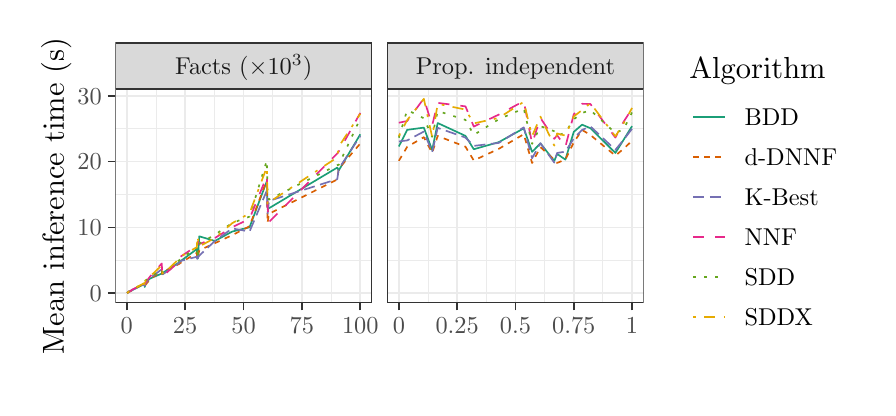
\begin{tikzpicture}[x=1pt,y=1pt]
\definecolor{fillColor}{RGB}{255,255,255}
\path[use as bounding box,fill=fillColor,fill opacity=0.00] (0,0) rectangle (303.53,130.09);
\begin{scope}
\path[clip] (  0.00,  0.00) rectangle (303.53,130.09);
\definecolor{drawColor}{RGB}{255,255,255}
\definecolor{fillColor}{RGB}{255,255,255}

\path[draw=drawColor,line width= 0.6pt,line join=round,line cap=round,fill=fillColor] (  0.00,  0.00) rectangle (303.53,130.09);
\end{scope}
\begin{scope}
\path[clip] ( 31.71, 30.69) rectangle (124.41,108.01);
\definecolor{fillColor}{RGB}{255,255,255}

\path[fill=fillColor] ( 31.71, 30.69) rectangle (124.41,108.01);
\definecolor{drawColor}{gray}{0.92}

\path[draw=drawColor,line width= 0.3pt,line join=round] ( 31.71, 46.03) --
	(124.41, 46.03);

\path[draw=drawColor,line width= 0.3pt,line join=round] ( 31.71, 69.81) --
	(124.41, 69.81);

\path[draw=drawColor,line width= 0.3pt,line join=round] ( 31.71, 93.59) --
	(124.41, 93.59);

\path[draw=drawColor,line width= 0.3pt,line join=round] ( 46.35, 30.69) --
	( 46.35,108.01);

\path[draw=drawColor,line width= 0.3pt,line join=round] ( 67.45, 30.69) --
	( 67.45,108.01);

\path[draw=drawColor,line width= 0.3pt,line join=round] ( 88.54, 30.69) --
	( 88.54,108.01);

\path[draw=drawColor,line width= 0.3pt,line join=round] (109.64, 30.69) --
	(109.64,108.01);

\path[draw=drawColor,line width= 0.6pt,line join=round] ( 31.71, 34.14) --
	(124.41, 34.14);

\path[draw=drawColor,line width= 0.6pt,line join=round] ( 31.71, 57.92) --
	(124.41, 57.92);

\path[draw=drawColor,line width= 0.6pt,line join=round] ( 31.71, 81.70) --
	(124.41, 81.70);

\path[draw=drawColor,line width= 0.6pt,line join=round] ( 31.71,105.48) --
	(124.41,105.48);

\path[draw=drawColor,line width= 0.6pt,line join=round] ( 35.80, 30.69) --
	( 35.80,108.01);

\path[draw=drawColor,line width= 0.6pt,line join=round] ( 56.90, 30.69) --
	( 56.90,108.01);

\path[draw=drawColor,line width= 0.6pt,line join=round] ( 78.00, 30.69) --
	( 78.00,108.01);

\path[draw=drawColor,line width= 0.6pt,line join=round] ( 99.09, 30.69) --
	( 99.09,108.01);

\path[draw=drawColor,line width= 0.6pt,line join=round] (120.19, 30.69) --
	(120.19,108.01);
\definecolor{drawColor}{RGB}{27,158,119}

\path[draw=drawColor,line width= 0.6pt,line join=round] ( 35.93, 34.22) --
	( 36.05, 34.28) --
	( 36.31, 34.45) --
	( 36.64, 34.74) --
	( 36.81, 34.74) --
	( 37.82, 35.27) --
	( 42.19, 37.45) --
	( 42.32, 36.38) --
	( 42.57, 37.84) --
	( 44.24, 39.46) --
	( 48.46, 41.24) --
	( 48.58, 41.31) --
	( 48.84, 41.51) --
	( 54.85, 45.33) --
	( 55.10, 45.62) --
	( 61.12, 50.08) --
	( 61.24, 47.64) --
	( 61.37, 50.15) --
	( 61.50, 46.59) --
	( 62.00, 54.70) --
	( 67.64, 53.02) --
	( 73.90, 56.41) --
	( 80.17, 57.95) --
	( 86.43, 74.63) --
	( 86.69, 65.78) --
	( 87.19, 64.84) --
	(111.88, 79.54) --
	(112.39, 78.48) --
	(120.19, 91.54);
\definecolor{drawColor}{RGB}{217,95,2}

\path[draw=drawColor,line width= 0.6pt,dash pattern=on 2pt off 2pt ,line join=round] ( 35.93, 34.20) --
	( 36.05, 34.26) --
	( 36.31, 34.41) --
	( 36.64, 34.70) --
	( 36.81, 34.68) --
	( 37.82, 35.23) --
	( 42.19, 37.74) --
	( 42.32, 37.05) --
	( 42.57, 37.14) --
	( 44.24, 39.19) --
	( 48.46, 42.35) --
	( 48.58, 40.98) --
	( 48.84, 41.86) --
	( 54.85, 44.75) --
	( 55.10, 45.01) --
	( 61.12, 48.70) --
	( 61.24, 46.51) --
	( 61.37, 47.05) --
	( 61.50, 47.32) --
	( 62.00, 49.64) --
	( 67.64, 52.22) --
	( 73.90, 55.11) --
	( 80.17, 58.33) --
	( 86.43, 75.16) --
	( 86.69, 59.59) --
	( 87.19, 62.82) --
	(111.88, 75.24) --
	(112.39, 79.11) --
	(120.19, 88.23);
\definecolor{drawColor}{RGB}{117,112,179}

\path[draw=drawColor,line width= 0.6pt,dash pattern=on 4pt off 2pt ,line join=round] ( 35.93, 34.22) --
	( 36.05, 34.33) --
	( 36.31, 34.49) --
	( 36.64, 34.77) --
	( 36.81, 34.77) --
	( 37.82, 35.37) --
	( 42.19, 37.40) --
	( 42.32, 36.84) --
	( 42.57, 37.68) --
	( 44.24, 39.58) --
	( 48.46, 42.81) --
	( 48.58, 41.77) --
	( 48.84, 40.98) --
	( 54.85, 45.16) --
	( 55.10, 45.74) --
	( 61.12, 47.31) --
	( 61.24, 46.52) --
	( 61.37, 48.59) --
	( 61.50, 46.96) --
	( 62.00, 47.72) --
	( 67.64, 52.99) --
	( 73.90, 57.55) --
	( 80.17, 56.42) --
	( 86.43, 71.23) --
	( 86.69, 62.93) --
	( 87.19, 67.49) --
	(111.88, 75.36) --
	(112.39, 79.09) --
	(120.19, 90.92);
\definecolor{drawColor}{RGB}{231,41,138}

\path[draw=drawColor,line width= 0.6pt,dash pattern=on 4pt off 4pt ,line join=round] ( 35.93, 34.22) --
	( 36.05, 34.29) --
	( 36.31, 34.48) --
	( 36.64, 34.79) --
	( 36.81, 34.74) --
	( 37.82, 35.45) --
	( 42.19, 37.64) --
	( 42.32, 37.18) --
	( 42.57, 37.98) --
	( 44.24, 40.20) --
	( 48.46, 44.88) --
	( 48.58, 42.06) --
	( 48.84, 40.35) --
	( 54.85, 45.65) --
	( 55.10, 47.25) --
	( 61.12, 51.25) --
	( 61.24, 51.16) --
	( 61.37, 51.25) --
	( 61.50, 52.79) --
	( 62.00, 51.87) --
	( 67.64, 54.08) --
	( 73.90, 57.97) --
	( 80.17, 61.03) --
	( 86.43, 76.47) --
	( 86.69, 65.20) --
	( 87.19, 59.83) --
	(111.88, 84.66) --
	(112.39, 85.31) --
	(120.19, 99.29);
\definecolor{drawColor}{RGB}{102,166,30}

\path[draw=drawColor,line width= 0.6pt,dash pattern=on 1pt off 3pt ,line join=round] ( 35.93, 34.24) --
	( 36.05, 34.31) --
	( 36.31, 34.48) --
	( 36.64, 34.81) --
	( 36.81, 34.77) --
	( 37.82, 35.45) --
	( 42.19, 37.88) --
	( 42.32, 38.54) --
	( 42.57, 38.69) --
	( 44.24, 39.95) --
	( 48.46, 42.70) --
	( 48.58, 41.93) --
	( 48.84, 41.20) --
	( 54.85, 46.14) --
	( 55.10, 46.43) --
	( 61.12, 50.70) --
	( 61.24, 47.87) --
	( 61.37, 50.28) --
	( 61.50, 47.98) --
	( 62.00, 52.07) --
	( 67.64, 55.24) --
	( 73.90, 59.51) --
	( 80.17, 61.81) --
	( 86.43, 82.15) --
	( 86.69, 68.77) --
	( 87.19, 67.98) --
	(111.88, 80.43) --
	(112.39, 80.51) --
	(120.19, 97.30);
\definecolor{drawColor}{RGB}{230,171,2}

\path[draw=drawColor,line width= 0.6pt,dash pattern=on 1pt off 3pt on 4pt off 3pt ,line join=round] ( 35.93, 34.20) --
	( 36.05, 34.32) --
	( 36.31, 34.47) --
	( 36.64, 34.80) --
	( 36.81, 34.78) --
	( 37.82, 35.44) --
	( 42.19, 37.83) --
	( 42.32, 36.07) --
	( 42.57, 38.73) --
	( 44.24, 40.20) --
	( 48.46, 44.23) --
	( 48.58, 43.29) --
	( 48.84, 40.97) --
	( 54.85, 46.70) --
	( 55.10, 47.28) --
	( 61.12, 50.76) --
	( 61.24, 52.81) --
	( 61.37, 51.86) --
	( 61.50, 53.84) --
	( 62.00, 51.03) --
	( 67.64, 54.08) --
	( 73.90, 59.44) --
	( 80.17, 63.01) --
	( 86.43, 79.72) --
	( 86.69, 66.18) --
	( 87.19, 66.97) --
	(111.88, 83.22) --
	(112.39, 87.08) --
	(120.19, 98.99);
\definecolor{drawColor}{gray}{0.20}

\path[draw=drawColor,line width= 0.6pt,line join=round,line cap=round] ( 31.71, 30.69) rectangle (124.41,108.01);
\end{scope}
\begin{scope}
\path[clip] (129.91, 30.69) rectangle (222.60,108.01);
\definecolor{fillColor}{RGB}{255,255,255}

\path[fill=fillColor] (129.91, 30.69) rectangle (222.60,108.01);
\definecolor{drawColor}{gray}{0.92}

\path[draw=drawColor,line width= 0.3pt,line join=round] (129.91, 46.03) --
	(222.60, 46.03);

\path[draw=drawColor,line width= 0.3pt,line join=round] (129.91, 69.81) --
	(222.60, 69.81);

\path[draw=drawColor,line width= 0.3pt,line join=round] (129.91, 93.59) --
	(222.60, 93.59);

\path[draw=drawColor,line width= 0.3pt,line join=round] (144.65, 30.69) --
	(144.65,108.01);

\path[draw=drawColor,line width= 0.3pt,line join=round] (165.72, 30.69) --
	(165.72,108.01);

\path[draw=drawColor,line width= 0.3pt,line join=round] (186.79, 30.69) --
	(186.79,108.01);

\path[draw=drawColor,line width= 0.3pt,line join=round] (207.85, 30.69) --
	(207.85,108.01);

\path[draw=drawColor,line width= 0.6pt,line join=round] (129.91, 34.14) --
	(222.60, 34.14);

\path[draw=drawColor,line width= 0.6pt,line join=round] (129.91, 57.92) --
	(222.60, 57.92);

\path[draw=drawColor,line width= 0.6pt,line join=round] (129.91, 81.70) --
	(222.60, 81.70);

\path[draw=drawColor,line width= 0.6pt,line join=round] (129.91,105.48) --
	(222.60,105.48);

\path[draw=drawColor,line width= 0.6pt,line join=round] (134.12, 30.69) --
	(134.12,108.01);

\path[draw=drawColor,line width= 0.6pt,line join=round] (155.19, 30.69) --
	(155.19,108.01);

\path[draw=drawColor,line width= 0.6pt,line join=round] (176.25, 30.69) --
	(176.25,108.01);

\path[draw=drawColor,line width= 0.6pt,line join=round] (197.32, 30.69) --
	(197.32,108.01);

\path[draw=drawColor,line width= 0.6pt,line join=round] (218.39, 30.69) --
	(218.39,108.01);
\definecolor{drawColor}{RGB}{27,158,119}

\path[draw=drawColor,line width= 0.6pt,line join=round] (134.12, 87.17) --
	(137.13, 93.17) --
	(143.15, 93.97) --
	(146.16, 85.86) --
	(148.16, 95.63) --
	(158.20, 90.99) --
	(161.20, 86.16) --
	(170.23, 88.72) --
	(179.26, 93.71) --
	(182.27, 85.21) --
	(185.28, 88.26) --
	(190.30, 81.94) --
	(191.30, 84.46) --
	(194.31, 82.43) --
	(197.32, 92.42) --
	(200.33, 95.04) --
	(203.34, 93.76) --
	(212.37, 84.82) --
	(215.38, 89.64) --
	(218.39, 94.51);
\definecolor{drawColor}{RGB}{217,95,2}

\path[draw=drawColor,line width= 0.6pt,dash pattern=on 2pt off 2pt ,line join=round] (134.12, 81.98) --
	(137.13, 87.03) --
	(143.15, 90.51) --
	(146.16, 84.86) --
	(148.16, 90.95) --
	(158.20, 87.07) --
	(161.20, 82.10) --
	(170.23, 86.31) --
	(179.26, 91.58) --
	(182.27, 81.17) --
	(185.28, 86.92) --
	(190.30, 82.36) --
	(191.30, 81.20) --
	(194.31, 82.46) --
	(197.32, 88.61) --
	(200.33, 93.14) --
	(203.34, 91.31) --
	(212.37, 83.85) --
	(215.38, 86.37) --
	(218.39, 89.25);
\definecolor{drawColor}{RGB}{117,112,179}

\path[draw=drawColor,line width= 0.6pt,dash pattern=on 4pt off 2pt ,line join=round] (134.12, 88.97) --
	(137.13, 89.35) --
	(143.15, 92.54) --
	(146.16, 85.10) --
	(148.16, 93.89) --
	(158.20, 90.38) --
	(161.20, 87.37) --
	(170.23, 88.45) --
	(179.26, 94.07) --
	(182.27, 82.90) --
	(185.28, 88.35) --
	(190.30, 81.32) --
	(191.30, 84.81) --
	(194.31, 85.30) --
	(197.32, 90.02) --
	(200.33, 93.14) --
	(203.34, 94.41) --
	(212.37, 85.94) --
	(215.38, 89.62) --
	(218.39, 93.56);
\definecolor{drawColor}{RGB}{231,41,138}

\path[draw=drawColor,line width= 0.6pt,dash pattern=on 4pt off 4pt ,line join=round] (134.12, 95.74) --
	(137.13, 96.35) --
	(143.15,104.50) --
	(146.16, 94.79) --
	(148.16,102.91) --
	(158.20,101.65) --
	(161.20, 94.35) --
	(170.23, 98.68) --
	(179.26,103.55) --
	(182.27, 88.20) --
	(185.28, 97.47) --
	(190.30, 89.92) --
	(191.30, 91.22) --
	(194.31, 87.06) --
	(197.32, 98.75) --
	(200.33,102.58) --
	(203.34,102.50) --
	(212.37, 90.37) --
	(215.38, 96.15) --
	(218.39,100.82);
\definecolor{drawColor}{RGB}{102,166,30}

\path[draw=drawColor,line width= 0.6pt,dash pattern=on 1pt off 3pt ,line join=round] (134.12, 90.34) --
	(137.13,100.33) --
	(143.15, 97.34) --
	(146.16, 90.63) --
	(148.16, 99.99) --
	(158.20, 96.75) --
	(161.20, 91.32) --
	(170.23, 97.00) --
	(179.26,100.90) --
	(182.27, 88.11) --
	(185.28, 94.51) --
	(190.30, 92.66) --
	(191.30, 90.99) --
	(194.31, 92.19) --
	(197.32, 96.98) --
	(200.33, 99.26) --
	(203.34,100.29) --
	(212.37, 92.01) --
	(215.38, 93.41) --
	(218.39, 99.52);
\definecolor{drawColor}{RGB}{230,171,2}

\path[draw=drawColor,line width= 0.6pt,dash pattern=on 1pt off 3pt on 4pt off 3pt ,line join=round] (134.12, 90.96) --
	(137.13, 96.67) --
	(143.15,104.39) --
	(146.16, 90.59) --
	(148.16,102.58) --
	(158.20,100.48) --
	(161.20, 95.50) --
	(170.23, 97.48) --
	(179.26,103.31) --
	(182.27, 90.87) --
	(185.28, 97.96) --
	(190.30, 87.48) --
	(191.30, 91.85) --
	(194.31, 91.08) --
	(197.32, 98.02) --
	(200.33,100.29) --
	(203.34,102.81) --
	(212.37, 90.81) --
	(215.38, 95.58) --
	(218.39,101.07);
\definecolor{drawColor}{gray}{0.20}

\path[draw=drawColor,line width= 0.6pt,line join=round,line cap=round] (129.91, 30.69) rectangle (222.60,108.01);
\end{scope}
\begin{scope}
\path[clip] ( 31.71,108.01) rectangle (124.41,124.59);
\definecolor{drawColor}{gray}{0.20}
\definecolor{fillColor}{gray}{0.85}

\path[draw=drawColor,line width= 0.6pt,line join=round,line cap=round,fill=fillColor] ( 31.71,108.01) rectangle (124.41,124.59);
\definecolor{drawColor}{gray}{0.10}

\node[text=drawColor,anchor=base,inner sep=0pt, outer sep=0pt, scale=  0.88] at ( 78.06,113.27) {Facts ($\times 10^3$)};
\end{scope}
\begin{scope}
\path[clip] (129.91,108.01) rectangle (222.60,124.59);
\definecolor{drawColor}{gray}{0.20}
\definecolor{fillColor}{gray}{0.85}

\path[draw=drawColor,line width= 0.6pt,line join=round,line cap=round,fill=fillColor] (129.91,108.01) rectangle (222.60,124.59);
\definecolor{drawColor}{gray}{0.10}

\node[text=drawColor,anchor=base,inner sep=0pt, outer sep=0pt, scale=  0.88] at (176.25,113.27) {Prop. independent};
\end{scope}
\begin{scope}
\path[clip] (  0.00,  0.00) rectangle (303.53,130.09);
\definecolor{drawColor}{gray}{0.20}

\path[draw=drawColor,line width= 0.6pt,line join=round] ( 35.80, 27.94) --
	( 35.80, 30.69);

\path[draw=drawColor,line width= 0.6pt,line join=round] ( 56.90, 27.94) --
	( 56.90, 30.69);

\path[draw=drawColor,line width= 0.6pt,line join=round] ( 78.00, 27.94) --
	( 78.00, 30.69);

\path[draw=drawColor,line width= 0.6pt,line join=round] ( 99.09, 27.94) --
	( 99.09, 30.69);

\path[draw=drawColor,line width= 0.6pt,line join=round] (120.19, 27.94) --
	(120.19, 30.69);
\end{scope}
\begin{scope}
\path[clip] (  0.00,  0.00) rectangle (303.53,130.09);
\definecolor{drawColor}{gray}{0.30}

\node[text=drawColor,anchor=base,inner sep=0pt, outer sep=0pt, scale=  0.88] at ( 35.80, 19.68) {0};

\node[text=drawColor,anchor=base,inner sep=0pt, outer sep=0pt, scale=  0.88] at ( 56.90, 19.68) {25};

\node[text=drawColor,anchor=base,inner sep=0pt, outer sep=0pt, scale=  0.88] at ( 78.00, 19.68) {50};

\node[text=drawColor,anchor=base,inner sep=0pt, outer sep=0pt, scale=  0.88] at ( 99.09, 19.68) {75};

\node[text=drawColor,anchor=base,inner sep=0pt, outer sep=0pt, scale=  0.88] at (120.19, 19.68) {100};
\end{scope}
\begin{scope}
\path[clip] (  0.00,  0.00) rectangle (303.53,130.09);
\definecolor{drawColor}{gray}{0.20}

\path[draw=drawColor,line width= 0.6pt,line join=round] (134.12, 27.94) --
	(134.12, 30.69);

\path[draw=drawColor,line width= 0.6pt,line join=round] (155.19, 27.94) --
	(155.19, 30.69);

\path[draw=drawColor,line width= 0.6pt,line join=round] (176.25, 27.94) --
	(176.25, 30.69);

\path[draw=drawColor,line width= 0.6pt,line join=round] (197.32, 27.94) --
	(197.32, 30.69);

\path[draw=drawColor,line width= 0.6pt,line join=round] (218.39, 27.94) --
	(218.39, 30.69);
\end{scope}
\begin{scope}
\path[clip] (  0.00,  0.00) rectangle (303.53,130.09);
\definecolor{drawColor}{gray}{0.30}

\node[text=drawColor,anchor=base,inner sep=0pt, outer sep=0pt, scale=  0.88] at (134.12, 19.68) {0};

\node[text=drawColor,anchor=base,inner sep=0pt, outer sep=0pt, scale=  0.88] at (155.19, 19.68) {0.25};

\node[text=drawColor,anchor=base,inner sep=0pt, outer sep=0pt, scale=  0.88] at (176.25, 19.68) {0.5};

\node[text=drawColor,anchor=base,inner sep=0pt, outer sep=0pt, scale=  0.88] at (197.32, 19.68) {0.75};

\node[text=drawColor,anchor=base,inner sep=0pt, outer sep=0pt, scale=  0.88] at (218.39, 19.68) {1};
\end{scope}
\begin{scope}
\path[clip] (  0.00,  0.00) rectangle (303.53,130.09);
\definecolor{drawColor}{gray}{0.30}

\node[text=drawColor,anchor=base east,inner sep=0pt, outer sep=0pt, scale=  0.88] at ( 26.76, 31.11) {0};

\node[text=drawColor,anchor=base east,inner sep=0pt, outer sep=0pt, scale=  0.88] at ( 26.76, 54.89) {10};

\node[text=drawColor,anchor=base east,inner sep=0pt, outer sep=0pt, scale=  0.88] at ( 26.76, 78.67) {20};

\node[text=drawColor,anchor=base east,inner sep=0pt, outer sep=0pt, scale=  0.88] at ( 26.76,102.45) {30};
\end{scope}
\begin{scope}
\path[clip] (  0.00,  0.00) rectangle (303.53,130.09);
\definecolor{drawColor}{gray}{0.20}

\path[draw=drawColor,line width= 0.6pt,line join=round] ( 28.96, 34.14) --
	( 31.71, 34.14);

\path[draw=drawColor,line width= 0.6pt,line join=round] ( 28.96, 57.92) --
	( 31.71, 57.92);

\path[draw=drawColor,line width= 0.6pt,line join=round] ( 28.96, 81.70) --
	( 31.71, 81.70);

\path[draw=drawColor,line width= 0.6pt,line join=round] ( 28.96,105.48) --
	( 31.71,105.48);
\end{scope}
\begin{scope}
\path[clip] (  0.00,  0.00) rectangle (303.53,130.09);
\definecolor{drawColor}{RGB}{0,0,0}

\node[text=drawColor,rotate= 90.00,anchor=base,inner sep=0pt, outer sep=0pt, scale=  1.10] at ( 13.08, 69.35) {Mean inference time (s)};
\end{scope}
\begin{scope}
\path[clip] (  0.00,  0.00) rectangle (303.53,130.09);
\definecolor{fillColor}{RGB}{255,255,255}

\path[fill=fillColor] (233.60, 12.88) rectangle (298.03,125.82);
\end{scope}
\begin{scope}
\path[clip] (  0.00,  0.00) rectangle (303.53,130.09);
\definecolor{drawColor}{RGB}{0,0,0}

\node[text=drawColor,anchor=base west,inner sep=0pt, outer sep=0pt, scale=  1.10] at (239.10,111.67) {Algorithm};
\end{scope}
\begin{scope}
\path[clip] (  0.00,  0.00) rectangle (303.53,130.09);
\definecolor{fillColor}{RGB}{255,255,255}

\path[fill=fillColor] (239.10, 90.65) rectangle (253.55,105.10);
\end{scope}
\begin{scope}
\path[clip] (  0.00,  0.00) rectangle (303.53,130.09);
\definecolor{drawColor}{RGB}{27,158,119}

\path[draw=drawColor,line width= 0.6pt,line join=round] (240.54, 97.88) -- (252.11, 97.88);
\end{scope}
\begin{scope}
\path[clip] (  0.00,  0.00) rectangle (303.53,130.09);
\definecolor{fillColor}{RGB}{255,255,255}

\path[fill=fillColor] (239.10, 76.20) rectangle (253.55, 90.65);
\end{scope}
\begin{scope}
\path[clip] (  0.00,  0.00) rectangle (303.53,130.09);
\definecolor{drawColor}{RGB}{217,95,2}

\path[draw=drawColor,line width= 0.6pt,dash pattern=on 2pt off 2pt ,line join=round] (240.54, 83.42) -- (252.11, 83.42);
\end{scope}
\begin{scope}
\path[clip] (  0.00,  0.00) rectangle (303.53,130.09);
\definecolor{fillColor}{RGB}{255,255,255}

\path[fill=fillColor] (239.10, 61.74) rectangle (253.55, 76.20);
\end{scope}
\begin{scope}
\path[clip] (  0.00,  0.00) rectangle (303.53,130.09);
\definecolor{drawColor}{RGB}{117,112,179}

\path[draw=drawColor,line width= 0.6pt,dash pattern=on 4pt off 2pt ,line join=round] (240.54, 68.97) -- (252.11, 68.97);
\end{scope}
\begin{scope}
\path[clip] (  0.00,  0.00) rectangle (303.53,130.09);
\definecolor{fillColor}{RGB}{255,255,255}

\path[fill=fillColor] (239.10, 47.29) rectangle (253.55, 61.74);
\end{scope}
\begin{scope}
\path[clip] (  0.00,  0.00) rectangle (303.53,130.09);
\definecolor{drawColor}{RGB}{231,41,138}

\path[draw=drawColor,line width= 0.6pt,dash pattern=on 4pt off 4pt ,line join=round] (240.54, 54.52) -- (252.11, 54.52);
\end{scope}
\begin{scope}
\path[clip] (  0.00,  0.00) rectangle (303.53,130.09);
\definecolor{fillColor}{RGB}{255,255,255}

\path[fill=fillColor] (239.10, 32.83) rectangle (253.55, 47.29);
\end{scope}
\begin{scope}
\path[clip] (  0.00,  0.00) rectangle (303.53,130.09);
\definecolor{drawColor}{RGB}{102,166,30}

\path[draw=drawColor,line width= 0.6pt,dash pattern=on 1pt off 3pt ,line join=round] (240.54, 40.06) -- (252.11, 40.06);
\end{scope}
\begin{scope}
\path[clip] (  0.00,  0.00) rectangle (303.53,130.09);
\definecolor{fillColor}{RGB}{255,255,255}

\path[fill=fillColor] (239.10, 18.38) rectangle (253.55, 32.83);
\end{scope}
\begin{scope}
\path[clip] (  0.00,  0.00) rectangle (303.53,130.09);
\definecolor{drawColor}{RGB}{230,171,2}

\path[draw=drawColor,line width= 0.6pt,dash pattern=on 1pt off 3pt on 4pt off 3pt ,line join=round] (240.54, 25.61) -- (252.11, 25.61);
\end{scope}
\begin{scope}
\path[clip] (  0.00,  0.00) rectangle (303.53,130.09);
\definecolor{drawColor}{RGB}{0,0,0}

\node[text=drawColor,anchor=base west,inner sep=0pt, outer sep=0pt, scale=  0.88] at (259.05, 94.85) {BDD};
\end{scope}
\begin{scope}
\path[clip] (  0.00,  0.00) rectangle (303.53,130.09);
\definecolor{drawColor}{RGB}{0,0,0}

\node[text=drawColor,anchor=base west,inner sep=0pt, outer sep=0pt, scale=  0.88] at (259.05, 80.39) {d-DNNF};
\end{scope}
\begin{scope}
\path[clip] (  0.00,  0.00) rectangle (303.53,130.09);
\definecolor{drawColor}{RGB}{0,0,0}

\node[text=drawColor,anchor=base west,inner sep=0pt, outer sep=0pt, scale=  0.88] at (259.05, 65.94) {K-Best};
\end{scope}
\begin{scope}
\path[clip] (  0.00,  0.00) rectangle (303.53,130.09);
\definecolor{drawColor}{RGB}{0,0,0}

\node[text=drawColor,anchor=base west,inner sep=0pt, outer sep=0pt, scale=  0.88] at (259.05, 51.49) {NNF};
\end{scope}
\begin{scope}
\path[clip] (  0.00,  0.00) rectangle (303.53,130.09);
\definecolor{drawColor}{RGB}{0,0,0}

\node[text=drawColor,anchor=base west,inner sep=0pt, outer sep=0pt, scale=  0.88] at (259.05, 37.03) {SDD};
\end{scope}
\begin{scope}
\path[clip] (  0.00,  0.00) rectangle (303.53,130.09);
\definecolor{drawColor}{RGB}{0,0,0}

\node[text=drawColor,anchor=base west,inner sep=0pt, outer sep=0pt, scale=  0.88] at (259.05, 22.58) {SDDX};
\end{scope}
\end{tikzpicture}
%
\end{frame}

\begin{frame}{Overview}
  \begin{block}{General parameters}
    \begin{itemize}
    \item maximum number of solutions
    \item \texttt{maxNumNodes} (in the tree representation of a clause)
    \item list of predicates with their variables
    \item maximum number of clauses
    \item option to forbid all cycles or just negative cycles
    \item list of probabilities that are randomly assigned to clauses: $\{ 0.1,
      0.2, \dots, 0.9, 1, 1, 1, 1, 1, 1 \}$
    \end{itemize}
  \end{block}
  \begin{block}{Decision variables}
    \begin{itemize}
    \item \texttt{IntVar[] clauseAssignments}: a predicate or disabled
    \item \texttt{Clause[] clauses}
    \end{itemize}
  \end{block}
\end{frame}

\begin{frame}{Constraints}
  \begin{block}{Each predicate should get at least one constraint}
    \begin{itemize}
    \item \texttt{numDisabledClauses}: defined by a \texttt{count} constraint
    \item $\texttt{numDistinctValues} = \begin{cases}
        \texttt{numPredicates} + 1 & \text{if } \texttt{numDisabledValues} > 0 \\
        \texttt{numPredicates} & \text{otherwise.}
      \end{cases}$
      \begin{itemize}
      \item also constrained using the \texttt{nValues} constraint
      \end{itemize}
    \end{itemize}
  \end{block}
  \begin{block}{Miscellaneous}
    \begin{itemize}
    \item \texttt{clauseAssignments} are sorted.
    \item If $\texttt{clauseAssignments}[i-1] = \texttt{clauseAssignments}[i]$,
      \begin{itemize}
      \item then $\texttt{clause}[i-1] \preceq \texttt{clause}[i]$.
      \end{itemize}
    \end{itemize}
  \end{block}
\end{frame}

\begin{frame}{Clauses}
  \begin{block}{A clause is defined by...}
    \begin{itemize}
    \item \texttt{IntVar[] treeStructure}
      \begin{itemize}
      \item $\texttt{treeStructure}[i] = i$: the $i$-th node is a root.
      \item $\texttt{treeStructure}[i] = j$: the $i$-th node's parent is node $j$.
      \end{itemize}
    \item \texttt{IntVar[] treeValues}: $\neg$, $\land$, $\lor$, $\top$, and any
      predefined predicates with variables.
    \end{itemize}
  \end{block}
  \begin{block}{Auxiliary variables}
    \begin{itemize}
    \item $\texttt{numNodes}, \texttt{numTrees} \in \{ 1, \dots, \texttt{maxNumNodes} \}$
    \end{itemize}
  \end{block}
\end{frame}

\begin{frame}{Clause constraints}
  \begin{itemize}
  \item \texttt{treeStructure} represents \texttt{numTrees} trees.
  \item $\texttt{treeStructure}[0] = 0$
  \item $\texttt{numTrees} + \texttt{numNodes} = \texttt{maxNumNodes} + 1$
  \item \texttt{treeStructure} is sorted
  \item For $i = 0, \dots, \texttt{maxNumNodes} - 1$,
    \begin{itemize}
    \item If $\texttt{numNodes} \le i$,
    \item then $\texttt{treeStructure}[i] = i$ and $\texttt{treeValues}[i] = \top$,
    \item else $\texttt{treeStructure}[i] < \texttt{numNodes}$.
    \item has 0 children $\iff$ $\texttt{treeValues}[i]$ is a predicate
    \item has 1 child $\iff$ $\texttt{treeValues}[i] = \neg$
    \item has $>1$ child $\iff$ $\texttt{treeValues}[i] \in \{ \land, \lor \}$
    \item $\texttt{treeStructure}[i] \ne i \implies \texttt{treeValues}[i] \ne \top$
    \end{itemize}
  \item If the clause should be disabled, $\texttt{numNodes} = 1$ and
    $\texttt{treeValues}[0] = \top$.
  \end{itemize}
\end{frame}

\begin{frame}
  \begin{block}{Adjacency matrix representation}
    $A[i][j] = 0 \iff \nexists k: \texttt{clauseAssignments}[k] = j$ and $i
    \in \texttt{clauses}[k].\texttt{treeValues}$
  \end{block}
  \begin{block}{New constraints}
    \begin{itemize}
    \item No (negative) cycles
      \begin{itemize}
      \item No clever propagation, just entailment checking.
      \end{itemize}
    \item Independence. Propagation:
      \begin{itemize}
      \item Two types of dependencies: determined and
        one-undetermined-edge-away-from-being-determined.
      \item Look up the dependencies of both predicates. For each pair of
        matching dependencies:
        \begin{itemize}
        \item If both are determined, fail.
        \item If one is determined, the selected edge of the other must not
          exist.
        \end{itemize}
      \end{itemize}
    \item Conditional independence
      \begin{itemize}
      \item Same propagation, but with a `filter' that masks out the expression
        that the independence is conditioned on.
      \end{itemize}
    \end{itemize}
  \end{block}
\end{frame}

\end{document}